%%%%%%%%%%%%%%%%%%%%%%%%%%%%%%%%%%%%%%%%%
% MSc BIS Thesis 
% LaTeX Template
% Version 1.0 (29/08/2014)
%
% Original authors:
% Steven Gunn 
% Sunil Patel
%
% Further authors:
% Michael Stauffer
% 
% This template is based on
% http://www.latextemplates.com/template/masters-doctoral-thesis
%
% License:
% CC BY-NC-SA 3.0 (http://creativecommons.org/licenses/by-nc-sa/3.0/)
%
%%%%%%%%%%%%%%%%%%%%%%%%%%%%%%%%%%%%%%%%%

%----------------------------------------------------------------------------------------
%	PACKAGES AND OTHER DOCUMENT CONFIGURATIONS
%----------------------------------------------------------------------------------------

% For digital publication it is recommended to use a one-sided layout
\documentclass[11pt, oneside]{Thesis}

% For printing it is recommended to use a two-sided layout
%\documentclass[11pt, twoside]{Thesis}

\makeglossaries

\begin{document}

%----------------------------------------------------------------------------------------
%	DOCUMENT VARIABLES
%	Fill in the lines below to update the thesis template
%	
%   If you want to cite each of the variables defined below, look at the
%	section above for the citation command.
%----------------------------------------------------------------------------------------

% You thesis title
% Citation command \thesisTitle
\thesisTitle{Enhanced Human-Banking-Interaction with Virtual Reality and Gesture Recognition}
%-------------------------------------------------  

% You supervisor's name 
% Citation command \supName 
\supervisor{Prof. Dr. Rolf \textsc{Dornberger}}
%-------------------------------------------------  

% You supervisor's URL
% Citation command \supURL
\supervisorURL{}
%-------------------------------------------------

% If you don't have a co-supervisor, exchange with
% \cosupervisorfalse
\cosupervisortrue
%-------------------------------------------------

% You co-supervisor's name 
% Citation command \supcoName 
\cosupervisor{Safak \textsc{Korkut}}
%-------------------------------------------------  

% You co-supervisor's URL
% Citation command \supcoURL
\cosupervisorURL{}
%-------------------------------------------------

% Your degree name
% Citation command \degreeName 
\degree{Master of Science in Business Information Systems}
%-------------------------------------------------   

% Your name
% Citation command \authorName
\authors{Fabian \textsc{Schär}}
%-------------------------------------------------

% Your URL
% Citation command \authorURL
\authorsURL{}
%-------------------------------------------------

% Your address (not used)
% Citation command \addressNames
\addresses{}
%-------------------------------------------------

% Your subject area (not used) 
% Citation command \subjectName
\subject{}
%-------------------------------------------------   

% Keywords for your thesis (not used)
% Citation command \keywordNames 
\keywords{}
%-------------------------------------------------

% http://www.fhnw.ch
% Citation command \fhnwURL 
%-------------------------------------------------

% University of Applied Sciences and Arts Northwestern Switzerland
% Citation command \fhnw 
%-------------------------------------------------

% UNIVERSITY OF APPLIED SCIENCES AND ARTS NORTHWESTERN SWITZERLAND
% Citation command \FHNW 
%-------------------------------------------------

% http://www.fhnw.ch/business
% Citation command \hswURL 
%-------------------------------------------------

% School of Business
% Citation command \hsw 
%-------------------------------------------------

% SCHOOL OF BUSINESS
% Citation command \HSW 
%-------------------------------------------------

% http://www.fhnw.ch/business/iwi
% Citation command \iwiURL 
%-------------------------------------------------

% Institute for Information Systems
% Citation command \iwi 
%-------------------------------------------------

% INSTITUTE FOR INFORMATION SYSTEMS for Information Systems
% Citation command \IWI
%-------------------------------------------------

%----------------------------------------------------------------------------------------
%	GLOSSARY
%	Add your glossary terms below
%	
%   If you want to cite a glossary term simply use \gls{term) for the singular form 
%   of the term or \glspl{term} for the plural form of the term.
%----------------------------------------------------------------------------------------

\newglossaryentry{Java}{
    name={Java},
    description={\blindtext}
}

\newglossaryentry{Oracle}{
    name={Oracle},
    description={\blindtext}
}

\newglossaryentry{Microsoft}{
    name={Microsoft},
    description={\blindtext}
}

%----------------------------------------------------------------------------------------
%	ABBREVIATIONS
%	Add your glossary terms below
%	
%   If you want to cite an abbreviation term simply use \gls{term) for the singular form  
%   of the term or \glspl{term} for the plural form of the term.
%----------------------------------------------------------------------------------------

\newacronym{svm}{SVM}{Support Vector Machine}


% PDF meta-data
\hypersetup{pdftitle={\thesisTitle}}
\hypersetup{pdfsubject=\subjectName}
\hypersetup{pdfauthor=\authorName}
\hypersetup{pdfkeywords=\keywordNames}

\frontmatter % Use roman page numbering style (i, ii, iii, iv...) for the pre-content pages

%----------------------------------------------------------------------------------------
%	TITLE PAGE
%----------------------------------------------------------------------------------------

\titlePage

%----------------------------------------------------------------------------------------
%	ABSTRACT PAGE
%----------------------------------------------------------------------------------------

\abstractPage{
    The Thesis Abstract is written here (and usually kept to just this page)\ldots
}

\clearpage % Start a new page

%----------------------------------------------------------------------------------------
%	FOREWORD / ACKNOWLEDGEMENTS (optional)
%----------------------------------------------------------------------------------------

\ackPage{
    The acknowledgements and the people to thank go here, don't forget to include your project advisor\ldots
}

\clearpage % Start a new page

%----------------------------------------------------------------------------------------
%	TABLE OF CONTENTS
%----------------------------------------------------------------------------------------

\tableofcontents

%----------------------------------------------------------------------------------------
%	THESIS CONTENT - CHAPTERS
%----------------------------------------------------------------------------------------

\mainmatter % Begin numeric (1,2,3...) page numbering

% Include the chapters of the thesis as separate files from the Chapters folder
% Uncomment the lines as you write the chapters

%\fillingPage{}
%%----------------------------------------------------------------------------------------
%	CHAPTER - HOW TO USE LATEX
%----------------------------------------------------------------------------------------

\chapter{Chapter Title Here} % Main chapter title

\label{Chapter1} % For referencing the chapter elsewhere, use \ref{Chapter1} 

%\lhead{Chapter x. \emph{Chapter Title Here}} % This is for the header on each page - perhaps a shortened title

%----------------------------------------------------------------------------------------

\section{Learning \LaTeX{}}

\LaTeX{} is not a WYSIWYG (What You See is What You Get) program, unlike word processors such as Microsoft Word or Apple's Pages. Instead, a document written for \LaTeX{} is actually a simple, plain text file that contains \emph{no formatting}. You tell \LaTeX{} how you want the formatting in the finished document by writing in simple commands amongst the text, for example, if I want to use \textit{italic text for emphasis}, I write the `$\backslash$\texttt{textit}\{\}' command and put the text I want in italics in between the curly braces. This means that \LaTeX{} is a ``mark-up'' language, very much like HTML.

\subsection{A (not so short) Introduction to \LaTeX{}}

If you are new to \LaTeX{}, there is a very good eBook -- freely available online as a PDF file -- called, ``The Not So Short Introduction to \LaTeX{}''. The book's title is typically shortened to just ``lshort''. You can download the latest version (as it is occasionally updated) from here:\\
\href{http://www.ctan.org/tex-archive/info/lshort/english/lshort.pdf}{\texttt{http://www.ctan.org/tex-archive/info/lshort/english/lshort.pdf}}

It is also available in several other languages. Find yours from the list on this page:\\
\href{http://www.ctan.org/tex-archive/info/lshort/}{\texttt{http://www.ctan.org/tex-archive/info/lshort/}}

It is recommended to take a little time out to learn how to use \LaTeX{} by creating several, small `test' documents. Making the effort now means you're not stuck learning the system when what you \emph{really} need to be doing is writing your thesis.

\subsection{A Short Math Guide for \LaTeX{}}

If you are writing a technical or mathematical thesis, then you may want to read the document by the AMS (American Mathematical Society) called, ``A Short Math Guide for \LaTeX{}''. It can be found online here:\\
\href{http://www.ams.org/tex/amslatex.html}{\texttt{http://www.ams.org/tex/amslatex.html}}\\
under the ``Additional Documentation'' section towards the bottom of the page.

\subsection{Common \LaTeX{} Math Symbols}
There are a multitude of mathematical symbols available for \LaTeX{} and it would take a great effort to learn the commands for them all. The most common ones you are likely to use are shown on this page:\\
\href{http://www.sunilpatel.co.uk/latexsymbols.html}{\texttt{http://www.sunilpatel.co.uk/latexsymbols.html}}

You can use this page as a reference or crib sheet, the symbols are rendered as large, high quality images so you can quickly find the \LaTeX{} command for the symbol you need.

%----------------------------------------------------------------------------------------

\section{What this Template Includes}

\subsection{Folders}

\textbf{01\_Chapters} -- this is the folder where you put the thesis chapters. The number of chapters is depending on the number of chapters needed for the \textit{Body of Text}. Each chapter should go in its own separate `\texttt{.tex}' file and they usually are split as:

\begin{itemize}
    \item Chapter 1: Introduction
    \item Chapter 2: Literature review
    \item Chapter 3: Research Method
    \item Chapter 4: Body of Text (1)
    \item Chapter 5: Body of Text (2)
    \item Chapter 6: Body of Text (3)
    \item Chapter 7: Conclusion
\end{itemize}

\textbf{02\_Appendices} -- this is the folder where you put the appendices. Each appendix should go into its own separate `\texttt{.tex}' file. A template is included in the directory.

\textbf{03\_Figures} -- this folder contains all figures (e.g.~pictures, diagrams, visualisations, etc.) for the thesis. These are the final images that will go into the thesis document.

\textbf{04\_Packages} -- this folder contains missing \LaTeX{} packages (`\texttt{.sty}' file) that are needed to compile this thesis document.

\subsection{Files}

Included are also several files, most of them are plain text and you can see their contents in a text editor. Luckily, many of them are auxiliary files created by \LaTeX{} or BibTeX and which you don't need to bother about:

\textbf{Bibliography.bib} -- this is an important file that contains all the bibliographic information and references that you will be citing in the thesis for use with BibTeX. You can write it manually, but there are reference manager programs available that will create and manage it for you. Bibliographies in \LaTeX{} are a large subject and you may need to read about BibTeX before starting with this.

\textbf{Thesis.cls} -- this is an important file. It is the style file that tells \LaTeX{} how to format the thesis. It is not necessary to change this file, so please leave it as it is.

\textbf{Author-Year-Title.pdf} -- this is your beautifully typeset thesis (in the PDF file format) created by \LaTeX{}.

\textbf{Author-Year-Title.tex} -- this is an important file. This is the file that you tell \LaTeX{} to compile to produce your thesis as a PDF file. It contains the framework and constructs that tell \LaTeX{} how to layout the thesis. It is heavily commented so you can read exactly what each line of code does and why it is there.

Files that are \emph{not} included, but are created by \LaTeX{} as auxiliary files include:

\textbf{Author-Year-Title.aux} -- this is an auxiliary file generated by \LaTeX{}, if it is deleted \LaTeX{} simply regenerates it when you run the main `\texttt{.tex}' file.

\textbf{Author-Year-Title.bbl} -- this is an auxiliary file generated by BibTeX, if it is deleted, BibTeX simply regenerates it when you run the main tex file. Whereas the `\texttt{.bib}' file contains all the references you have, this `\texttt{.bbl}' file contains the references you have actually cited in the thesis and is used to build the bibliography section of the thesis.

\textbf{Author-Year-Title.blg} -- this is an auxiliary file generated by BibTeX, if it is deleted BibTeX simply regenerates it when you run the main `\texttt{.tex}' file.

\textbf{Author-Year-Title.lof} -- this is an auxiliary file generated by \LaTeX{}, if it is deleted \LaTeX{} simply regenerates it when you run the main `\texttt{.tex}' file. It tells \LaTeX{} how to build the `List of Figures' section.

\textbf{Author-Year-Title.log} -- this is an auxiliary file generated by \LaTeX{}, if it is deleted \LaTeX{} simply regenerates it when you run the main `\texttt{.tex}' file. It contains messages from \LaTeX{}, if you receive errors and warnings from \LaTeX{}, they will be in this `\texttt{.log}' file.

\textbf{Author-Year-Title.lot} -- this is an auxiliary file generated by \LaTeX{}, if it is deleted \LaTeX{} simply regenerates it when you run the main `\texttt{.tex}' file. It tells \LaTeX{} how to build the `List of Tables' section.

\textbf{Author-Year-Title.out} -- this is an auxiliary file generated by \LaTeX{}, if it is deleted \LaTeX{} simply regenerates it when you run the main `\texttt{.tex}' file.

%----------------------------------------------------------------------------------------

\section{Thesis Features and Conventions}
\label{ThesisConventions}

\subsection{Printing Format}

This thesis template is designed for single sided printing as most theses are printed and bound this way. This means that the left margin is always wider than the right (for binding). Four out of five people will now judge the margins by eye and think, ``I never 
noticed that before.''.

The headers for the pages contain the page number on the right side (so it is easy to flick through to the page you want) and the chapter name on the left side.

The text is set to 11 point and a line spacing of 1.3. Generally, it is much more readable to have a smaller text size and wider gap between the lines than it is to have a larger text size and smaller gap.

\subsection{References}

The `\texttt{natbib}' package is used to format the bibliography and inserts references such as this one~\citep{Reference3}. The options used in this thesis mean that the references are listed in numerical order as they appear in the text. Multiple references are rearranged in numerical order e.g.~\citep{Reference2, Reference1} and multiple, sequential references become reformatted to a reference range e.g.~\citep{Reference2, Reference1, Reference3}. Further information regarding citation in LaTeX{} can be found \href{http://en.wikibooks.org/wiki/LaTeX/Bibliography_Management}{here}.

Did you know that also Mendeley is supporting \LaTeX{} ? If not have a look at this \href{http://blog.mendeley.com/tipstricks/howto-use-mendeley-to-create-citations-using-latex-and-bibtex/}{blog post} and get to know the power of these powerful tools. 

Scientific references should come \emph{before} the punctuation mark if there is one (such as a comma or period) together with a \verb!~! in front of the citation command. The same goes for footnotes\footnote{Such as this footnote, here down at the bottom of the page.}. You can change this but the most important thing is to keep the convention consistent throughout the thesis. Footnotes themselves should be full, descriptive sentences (beginning with a capital letter and ending with a full stop).

To see how \LaTeX{} typesets the bibliography, have a look at the very end of this document (or just click on the reference number links).

\subsection{Glossary and Abbreviations}

You can reference any glossary term that you have defined at the beginning of this document, by the following commands `$\backslash$\texttt{gls}' (singular) or `$\backslash$\texttt{glspl}' (plural). An example is provided below:

\gls{Java} is a object-oriented programming language that is maintained and released by \gls{Oracle}. \gls{Oracle}'s main competitor in this field is \gls{Microsoft}.

In addition to that is also possible to reference any abbreviations in the same way. However, if you reference an abbreviation the first time it will show you the full name plus the abbreviation itself in the brace. From the second time you reference the same abbreviation it will only show you the abbreviation itself. An example is provided below:

First use \gls{svm} and second use \gls{svm}.

Further information regarding glossary and abbreviations can be found \href{http://www.ctan.org/pkg/glossaries}{here} and \href{http://latex-community.org/know-how/latex/55-latex-general/263-glossaries-nomenclature-lists-of-symbols-and-acronyms}{here}.

\subsection{Figures}

There will hopefully be many figures in your thesis (that should be placed in the `03\_Figures' folder). The way to insert figures into your thesis is to use a code template like this:

\begin{verbatim}
\begin{figure}[htbp]
	\centering
		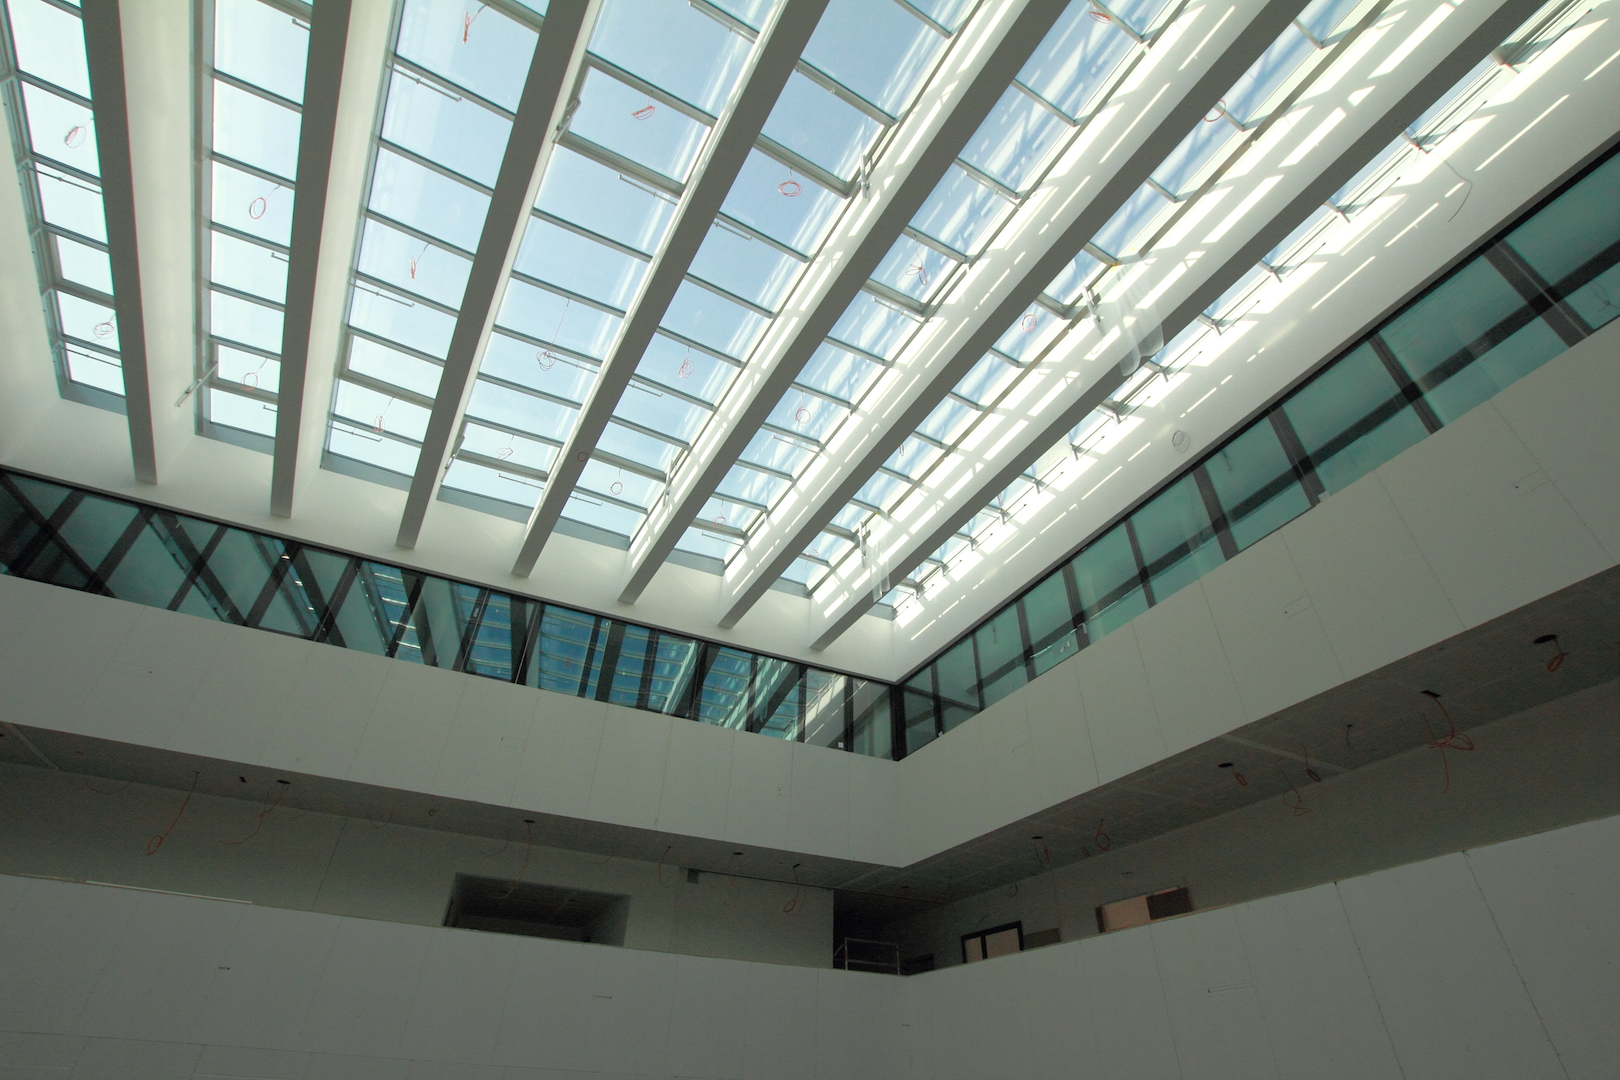
\includegraphics[width=13cm]{01_Campus/CampusOlten.jpeg}
		\rule{35em}{0.5pt}
	\caption[Campus Olten]{FHNW Campus Olten.}
	\label{fig:Campus}
\end{figure}
\end{verbatim}

Also look in the source file. Putting this code into the source file produces the picture of the electron that you can see in the figure below.

\begin{figure}[htbp]
	\centering
		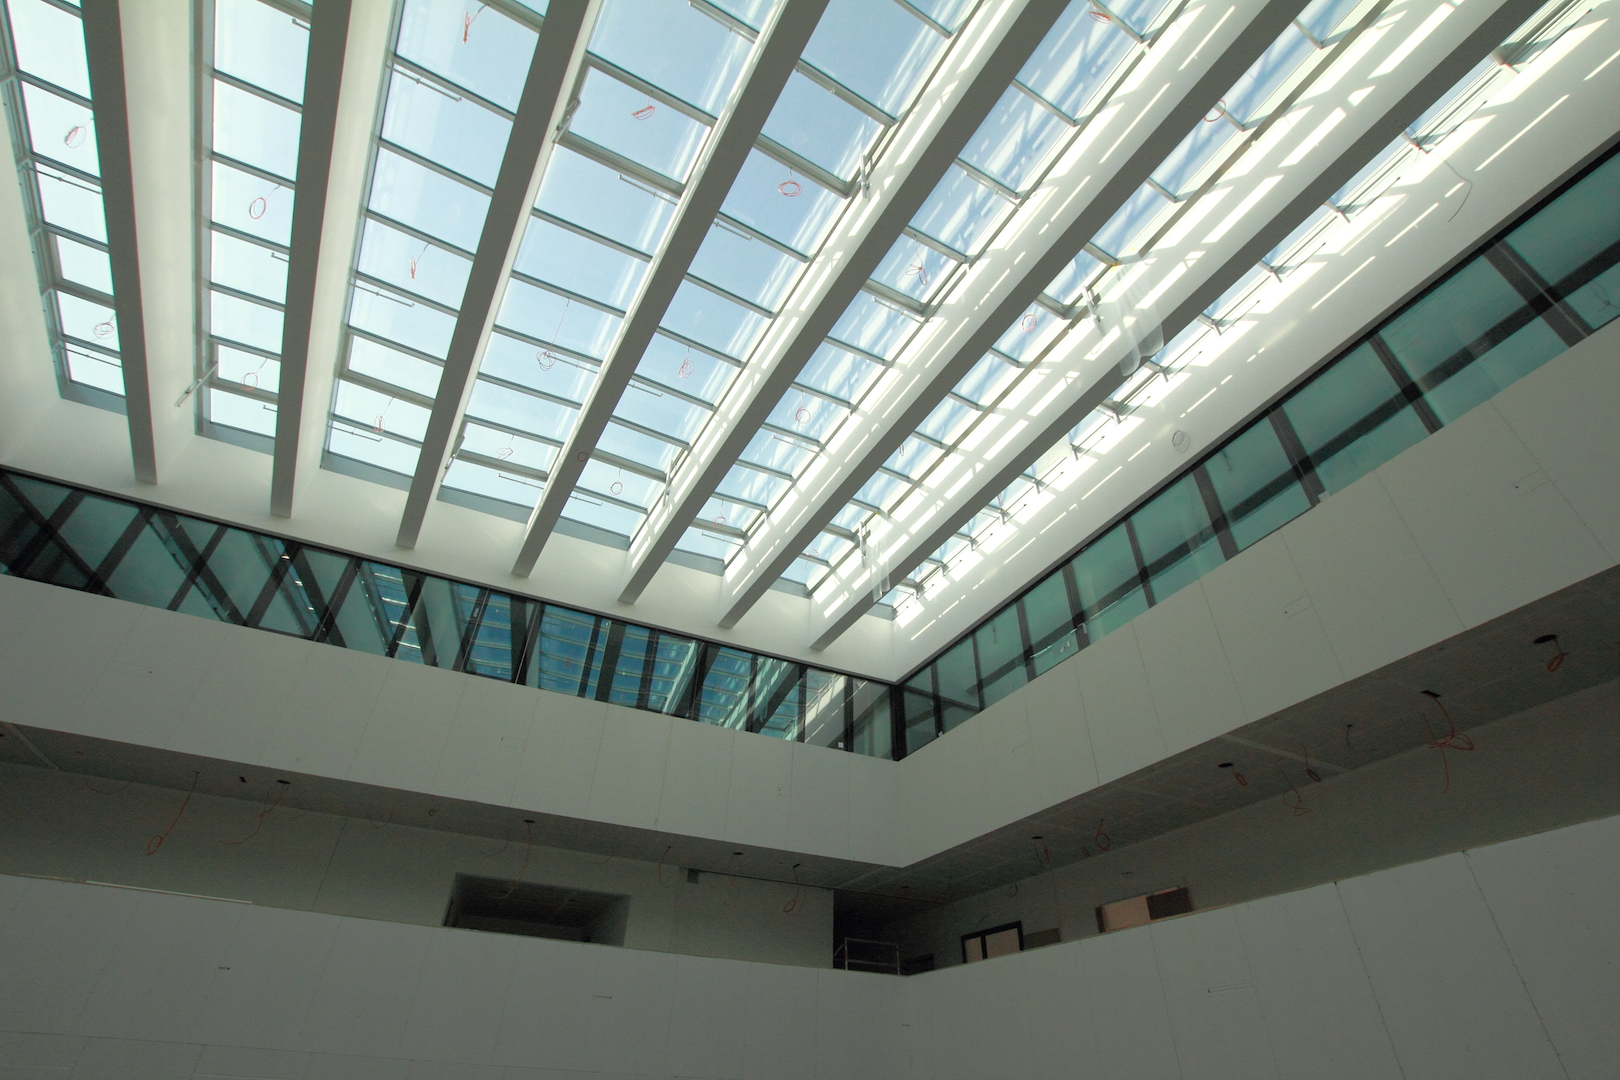
\includegraphics[width=10cm]{01_Campus/CampusOlten.jpeg}
		\rule{35em}{0.5pt}
	\caption[Campus Olten]{FHNW Campus Olten.}
	\label{fig:Campus}
\end{figure}

Sometimes figures don't always appear where you write them in the source. The placement depends on how much space there is on the page for the figure. Sometimes there is not enough room to fit a figure directly where it should go (in relation to the text) and so \LaTeX{} puts it at the top of the next page. Positioning figures is the job of \LaTeX{} and so you should only worry about making them look good!

Figures usually should have labels just in case you need to refer to them (such as in Figure \ref{fig:Campus}). The `$\backslash$\texttt{caption}' command contains two parts, the first part, inside the square brackets is the title that will appear in the `List of Figures', and so should be short. The second part in the curly brackets should contain the longer and more descriptive caption text.

The `$\backslash$\texttt{rule}' command is optional and simply puts an aesthetic horizontal line below the image. If you do this for one image, do it for all of them.

The \LaTeX{} Thesis Template is able to use figures that are either in the PDF or JPEG file format.

\subsection{Tables}

\LaTeX{} is capable to create beautiful tables from scratch, to improve them even more we implemented the \texttt{booktabs} package for you. Further information regarding this package and why it's not recommend to use horizontal lines can be found \href{http://texdoc.net/texmf-dist/doc/latex/booktabs/booktabs.pdf}{here}.

Tables are in many ways like figures as such it is also possible to define the position, to attach a caption or to add a label (see Table \ref{table:FHNWLocations}). The number of rows respectively their size and behaviour can be defined in the header of the within the `$\backslash$\texttt{tabular}' command. In this example we have defined two top-aligned paragraphs with a predefined size. Further row types and explanations can be found \href{http://en.wikibooks.org/wiki/LaTeX/Tables}{here}. 

The \texttt{booktabs} package offers furthermore the opportunity to define a horizontal line at the beginning (\verb!\toprule!), between (\verb!\midrule!) and the end (\verb!\bottomrule!) of the table. 

However, in order to start a new column you can simply add a \texttt{\$} at the end of your current column. In the same way you can also start a new row by adding a \verb!\\! at the end of your text.

\begin{table}[!h]
    \begin{tabular}{p{5cm} p{8cm}}

    \toprule
    
    \textbf{Schools} & \textbf{Locations}\\
    
    \midrule
    
    School of Applied Psychology & 
    Olten\\
    
    \midrule
    
    School of Business &
    Basel, Olten, Windisch\\
    
    \midrule
    
    School of Education &
    Aarau, Basel, Windisch, Liestal, Solothurn\\
    
    \midrule
    
    School of Engineering &
    Muttenz, Olten, Windisch\\
    
    \midrule
    
    School of Life Sciences &
    Muttenz\\
    
    \bottomrule
                         
    \end{tabular}
  \caption{Locations of the different schools of FHNW}
  \label{table:FHNWLocations}
\end{table}

\subsection{Typesetting mathematics}

If your thesis is going to contain heavy mathematical content, be sure that \LaTeX{} will make it look beautiful, even though it won't be able to solve the equations for you.

The ``Not So Short Introduction to \LaTeX{}'' (available \href{http://www.ctan.org/tex-archive/info/lshort/english/lshort.pdf}{here}) should tell you everything you need to know for most cases of typesetting mathematics. There are many different \LaTeX{} symbols to remember, luckily you can find the most common symbols \href{https://www.sharelatex.com/learn/List_of_Greek_letters_and_math_symbols}{here}.

You can write an equation, which is automatically given an equation number by \LaTeX{} like this:

\begin{verbatim}
\begin{equation}
E = mc^{2}
  \label{eqn:Einstein}
\end{equation}
\end{verbatim}

This will produce Einstein's famous energy-matter equivalence equation:
\begin{equation}
E = mc^{2}
\label{eqn:Einstein}
\end{equation}

All equations you write (which are not in the middle of paragraph text) are automatically given equation numbers by \LaTeX{}. If you don't want a particular equation numbered, just put the command, `$\backslash$\texttt{nonumber}' immediately after the equation.

Furthermore you can also write inline equations by inserting a `\$' in front and end of the equation, like that $E=mc^2$.

%----------------------------------------------------------------------------------------

\section{Sectioning and Subsectioning}

You should break your thesis up into nice, bite-sized sections and subsections. \LaTeX{} automatically builds a table of Contents by looking at all the `$\backslash$\texttt{chapter}$\{\}$', `$\backslash$\texttt{section}$\{\}$' and `$\backslash$\texttt{subsection}$\{\}$' commands you write in the source.

The table of Contents should only list the sections to three (3) levels. A `$\backslash$\texttt{chapter}$\{\}$' is level one (1). A `$\backslash$\texttt{section}$\{\}$' is level two (2) and so a `$\backslash$\texttt{subsection}$\{\}$' is level three (3). In your thesis it is likely that you will even use a `$\backslash$\texttt{subsubsection}$\{\}$', which is level four (4). Adding all these will create an unnecessarily cluttered table of Contents and so you should use the `$\backslash$\texttt{subsubsection$^{*}\{\}$}' command instead (note the asterisk). The asterisk ($^{*}$) tells \LaTeX{} to omit listing the subsubsection in the Contents, keeping it clean and tidy.

%----------------------------------------------------------------------------------------

\section{In Closing}

You have reached the end of this mini-guide. You can now remove this chapter (\texttt{00\_HowTo\\UseLatex.tex}) from your content in the \texttt{Author-Year-Title.tex} file and start writing your thesis. The easy work of setting up the structure and framework has been taken care of for you. It's now your job to fill it out!

\begin{flushright}
Guide written by Sunil Patel\\
and adapted by Michael Stauffer\\
\end{flushright}
 % Delete this line after reading this chapter

\fillingPage{}
%----------------------------------------------------------------------------------------
%	CHAPTER - INTRODUCTUION
%----------------------------------------------------------------------------------------

\chapter{Introduction} % Main chapter title

\label{ChapterIntroduction} % Change X to a consecutive number; for referencing this chapter elsewhere, use \ref{ChapterX}

%----------------------------------------------------------------------------------------
%	SECTION 1
%----------------------------------------------------------------------------------------

\section{Introduction}

Lorem ipsum dolor sit amet, consectetur adipiscing elit. Aliquam ultricies lacinia euismod. Nam tempus risus in dolor rhoncus in interdum enim tincidunt. Donec vel nunc neque. In condimentum ullamcorper quam non consequat. Fusce sagittis tempor feugiat. Fusce magna erat, molestie eu convallis ut, tempus sed arcu. Quisque molestie, ante a tincidunt ullamcorper, sapien enim dignissim lacus, in semper nibh erat lobortis purus. Integer dapibus ligula ac risus convallis pellentesque.   

%-----------------------------------
%	SUBSECTION 1
%-----------------------------------
\subsection{Subsection 1}

Nunc posuere quam at lectus tristique eu ultrices augue venenatis. Vestibulum ante ipsum primis in faucibus orci luctus et ultrices posuere cubilia Curae; Aliquam erat volutpat. Vivamus sodales tortor eget quam adipiscing in vulputate ante ullamcorper. Sed eros ante, lacinia et sollicitudin et, aliquam sit amet augue. In hac habitasse platea dictumst.

%-----------------------------------
%	SUBSECTION 2
%-----------------------------------

\subsection{Subsection 2}
Morbi rutrum odio eget arcu adipiscing sodales. Aenean et purus a est pulvinar pellentesque. Cras in elit neque, quis varius elit. Phasellus fringilla, nibh eu tempus venenatis, dolor elit posuere quam, quis adipiscing urna leo nec orci. Sed nec nulla auctor odio aliquet consequat. Ut nec nulla in ante ullamcorper aliquam at sed dolor. Phasellus fermentum magna in augue gravida cursus. Cras sed pretium lorem. Pellentesque eget ornare odio. Proin accumsan, massa viverra cursus pharetra, ipsum nisi lobortis velit, a malesuada dolor lorem eu neque.

%----------------------------------------------------------------------------------------
%	SECTION 2
%----------------------------------------------------------------------------------------

\section{Background}

Sed ullamcorper quam eu nisl interdum at interdum enim egestas. Aliquam placerat justo sed lectus lobortis ut porta nisl porttitor. Vestibulum mi dolor, lacinia molestie gravida at, tempus vitae ligula. Donec eget quam sapien, in viverra eros. Donec pellentesque justo a massa fringilla non vestibulum metus vestibulum. Vestibulum in orci quis felis tempor lacinia. Vivamus ornare ultrices facilisis. Ut hendrerit volutpat vulputate. Morbi condimentum venenatis augue, id porta ipsum vulputate in. Curabitur luctus tempus justo. Vestibulum risus lectus, adipiscing nec condimentum quis, condimentum nec nisl. Aliquam dictum sagittis velit sed iaculis. Morbi tristique augue sit amet nulla pulvinar id facilisis ligula mollis. Nam elit libero, tincidunt ut aliquam at, molestie in quam. Aenean rhoncus vehicula hendrerit.

%----------------------------------------------------------------------------------------
%	SECTION 3
%----------------------------------------------------------------------------------------

\section{Problem Statement}

blub


%----------------------------------------------------------------------------------------
%	SECTION 4
%----------------------------------------------------------------------------------------

\section{Thesis Statement}

blub


%----------------------------------------------------------------------------------------
%	SECTION 5
%----------------------------------------------------------------------------------------

\section{Research question}

blub


%----------------------------------------------------------------------------------------
%	SECTION 6
%----------------------------------------------------------------------------------------

\section{Research objectives}

blub


%----------------------------------------------------------------------------------------
%	SECTION 7
%----------------------------------------------------------------------------------------

\section{Short overview}

blub


%----------------------------------------------------------------------------------------
%	SECTION 8
%----------------------------------------------------------------------------------------

\section{Delineations and Limitations}

blub


%----------------------------------------------------------------------------------------
%	SECTION 9
%----------------------------------------------------------------------------------------

\section{Underlying Assumptions}

blub


%----------------------------------------------------------------------------------------
%	SECTION 10
%----------------------------------------------------------------------------------------

\section{Definition of terms and concepts}

blub


%----------------------------------------------------------------------------------------
%	SECTION 11
%----------------------------------------------------------------------------------------

\section{Significance}

blub

%-----------------------------------
%	SUBSECTION 1
%-----------------------------------

\subsection{Theoretical}

subblub


%-----------------------------------
%	SUBSECTION 2
%-----------------------------------

\subsection{Practical}

subblub


%----------------------------------------------------------------------------------------
%	SECTION 12
%----------------------------------------------------------------------------------------

\section{Thesis structure and brief chapter overviews}

blub


%----------------------------------------------------------------------------------------
%	SECTION 13
%----------------------------------------------------------------------------------------

\section{Any other institutional requirement not covered here}

blub




 

\fillingPage{}
%----------------------------------------------------------------------------------------
%	CHAPTER - LITERATURE REVIEW
%----------------------------------------------------------------------------------------

\chapter{Literature Review} % Main chapter title

\label{ChapterLiteratureReview} % Change X to a consecutive number; for referencing this chapter elsewhere, use \ref{ChapterX}

In the literature review chapter, an overview of existing research found in literature, that is relevant to the thesis statement of this paper, is given. Every \gls{srq} is discussed in its own sub-chapter where its relevance to the \gls{mrq} is elaborated. Each sub-chapter ends with a short conclusion and answers to the corresponding research question are given.
Figure \ref{fig:litreviewoverview} shows the correlation between the sub-chapters and the research questions. In chapter \ref{SectionLiteratureReviewSRQ1}, the different methods for user input in virtual reality are analysed The next chapter \ref{SectionLiteratureReviewSRQ2} focuses on existing data interaction patterns in virtual reality. By looking at strategies for the visualisation and manipulation of data, the third SRQ is covered in chapter \ref{SectionLiteratureReviewSRQ3}. To wrap everything up, a conclusion of the literature review is presented in chapter \ref{SectionLiteratureReviewConclusion} which builds the base for the research design in chapter \ref{Research Method}.
\newline
\begin{figure}[h]
	\begin{center}
		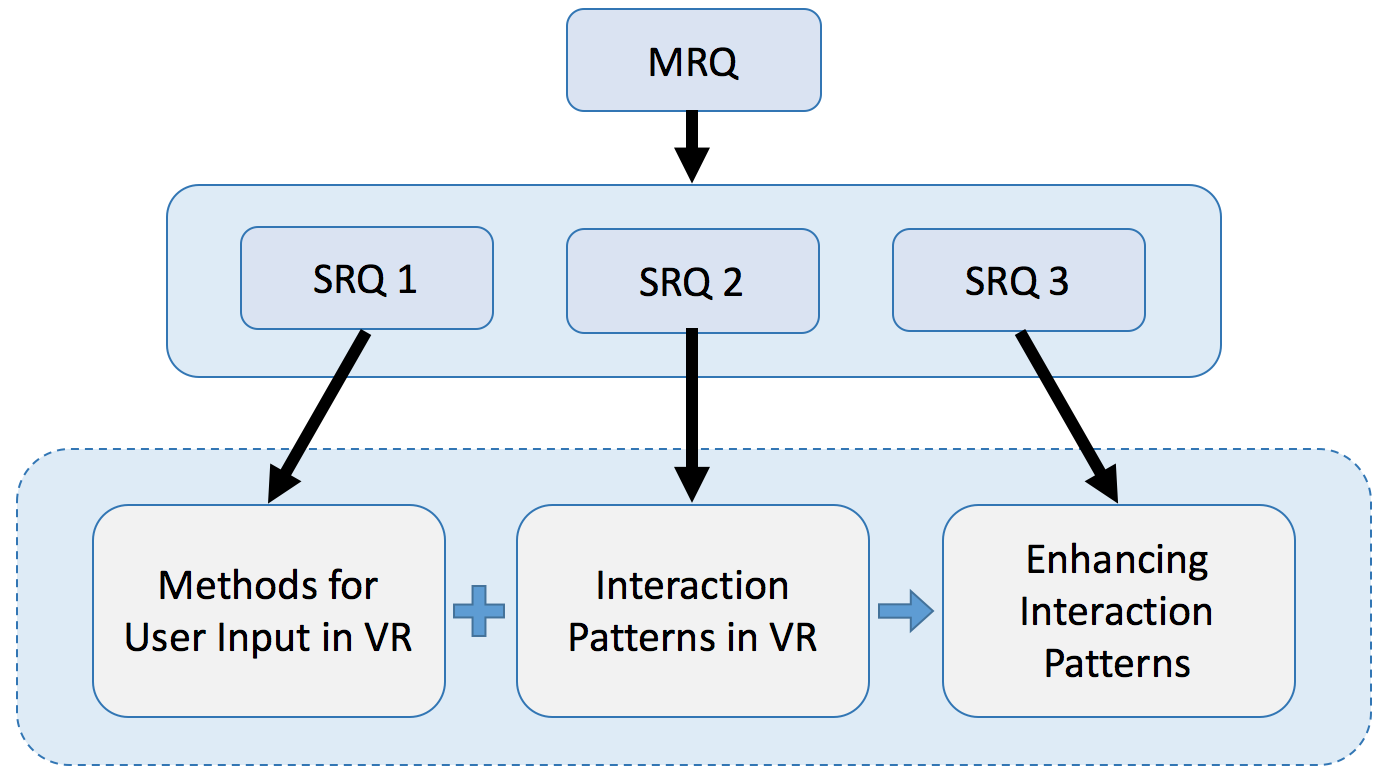
\includegraphics[width=12cm]{03_Figures/05_LitReview/LitReview_SRQ.png}
		\caption{Chapter 2 Overview}
		\label{fig:litreviewoverview}
	\end{center}
\end{figure}


%----------------------------------------------------------------------------------------
%	SECTION 1
%----------------------------------------------------------------------------------------

\section{Different Methods for User Input in Virtual Reality}

\label{SectionLiteratureReviewSRQ1}

This chapter deals with the first SRQ, focusing on the currently used and researched different methods for user input in virtual reality. It starts with an introduction and an overview of the different methods while the subsequent chapters give more details on the individual methods.
\begin{framed}
	\textit{SRQ 1: Which methods of user input in virtual reality are researched and what are their advantages and disadvantages?}
\end{framed}

%-----------------------------------
%	SUBSECTION 1
%-----------------------------------
\subsection{Introduction}

\gls{hci} itself has been worked and research on approximately from the 1950s onwards, where the main focus was on the direct manipulation of graphical objects with the mouse as well as gesture recognition \citep{Myers1998}. During this time however, gesture recognition was rather understood as devices that work with pen-based input devices and thus can recognize patterns that are drawn with these pens \citep{Myers1998}. In the regular interaction between human and machines these methods for user input are still fairly sufficient as even today we are completely relying on having a mouse/track-pad/touch-screen and a keyboard to interact with our devices. \newline
Virtual reality changes this quite a bit since wearing a \gls{hmd} with its own display obstructs the view on the so far used physical input devices. New solutions had to be found for this changed situation. An overview on the researched interaction patterns with virtual reality is shown in the following sub-chapter.


%-----------------------------------
%	SUBSECTION 2
%-----------------------------------

\subsection{Overview of the Different Methods}

The reviewed literature brought up different means in research to interact with the virtual reality environment. In order to review them in a more structured way, they have been grouped by their core technology (i.e. hand gestures, speech recognition etc.) on which they base on. Every core technology is discussed individually, its advantages and disadvantages are discussed, as well as their similarities or differences are explained.


\subsubsection{Hand Gestures}

\label{SubSubSectionHandGestures}

The by far most utilized and researched interaction method is hand gestures. Since we also heavily rely on this interaction pattern in real life with other human beings, it is fair to assume that the familiarity of it helps the research in a significant way whereas methods that rely on physical hardware often feel more distant. \newline
\cite{Pfeiffer2008} conducted an empirical study about conversational pointing gestures in virtual reality interaction where the focus lied on the system to recognize on which object the user was pointing at. \cite{Pfeiffer2008} distinguished between \gls{ifp} where the direction of where the index finger is pointing at, and \gls{gfp} where an imaginary line between the viewers eye and the tip of the index finger is drawn. Provided the objects are nod too close to each other (ca. 20cm), both methods had equal accuracy and success while tracked with two cameras from different angles and motion capturing \citep{Pfeiffer2008}. Figure \ref{fig:pointinggesture} shows the application of this in an identification game which was part of the empirical study.
\begin{figure}[h]
	\begin{center}
		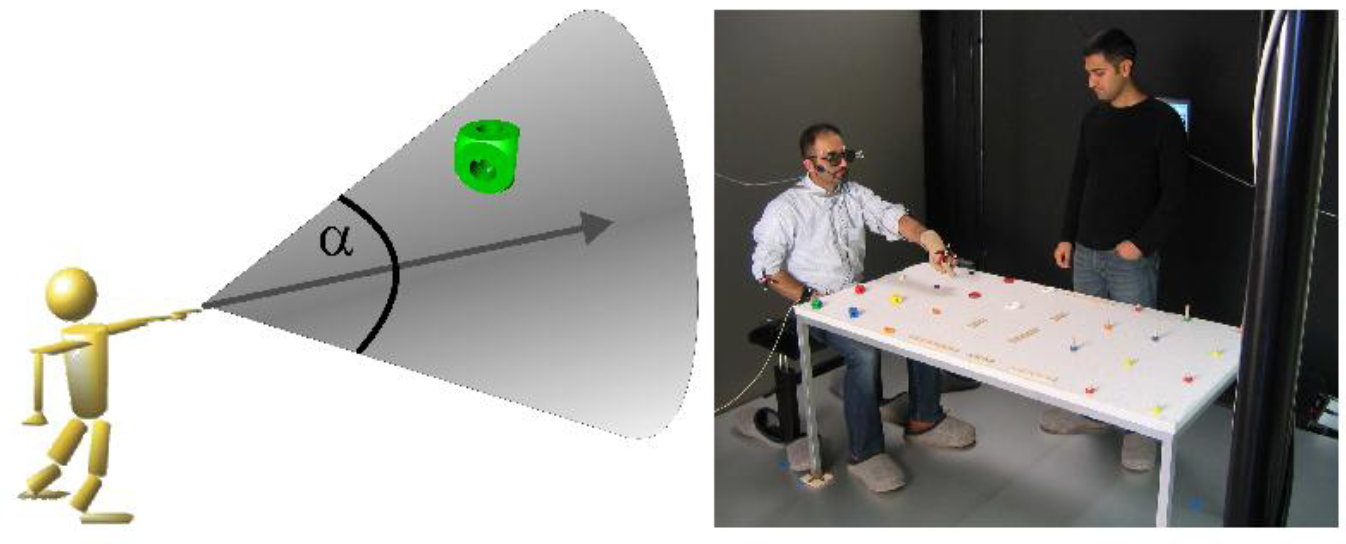
\includegraphics[width=10cm]{03_Figures/05_LitReview/Pfeiffer2008_Pointing.png}
		\caption[Cone-based model for extension of pointing gestures refined for identification game]{Cone-based model for extension of pointing gestures (left) refined for identification game (right) \citep{Pfeiffer2008}}
		\label{fig:pointinggesture}
	\end{center}
\end{figure}
\newline
A similar approach has been research by \cite{Rautaray2011} who used a single camera with an application that did the image capturing, locating the hand and its orientation and finally modelling the gesture to find a match for predefined gestures. The focus relied on simple gestures for \textit{punch} (three fingers), \textit{grab} (fist), \textit{throw} (five fingers), and to \textit{move forward} (thumb up) within a simple \gls{vr} game \citep{Rautaray2011}. The recognition rate was between 80\% and 94\% (depending on the gesture), which might not be accurate enough for practical use cases as also acknowledged by \cite{Rautaray2011}. \newline
In a more recent study of \cite{Khundam2015}, it was not cameras that were used to track the hand gestures but a Leap Motion (an in-air controller) attached to the front of an Oculus Rift. Figure \ref{fig:leapmotion} shows the different gestures that were implemented by \cite{Khundam2015} in order to navigate within a virtual environment. Depending on how far the hand is moved towards a certain angle, the speed of the movement can be influenced to increase or decrease it \citep{Khundam2015}. Although the applied gestures are understandable and easy to learn, they still bring some unfamiliarity with them since in real life movement already has a specific gesture which however utilizes the legs and not the hands.
\begin{figure}[h]
	\begin{center}
		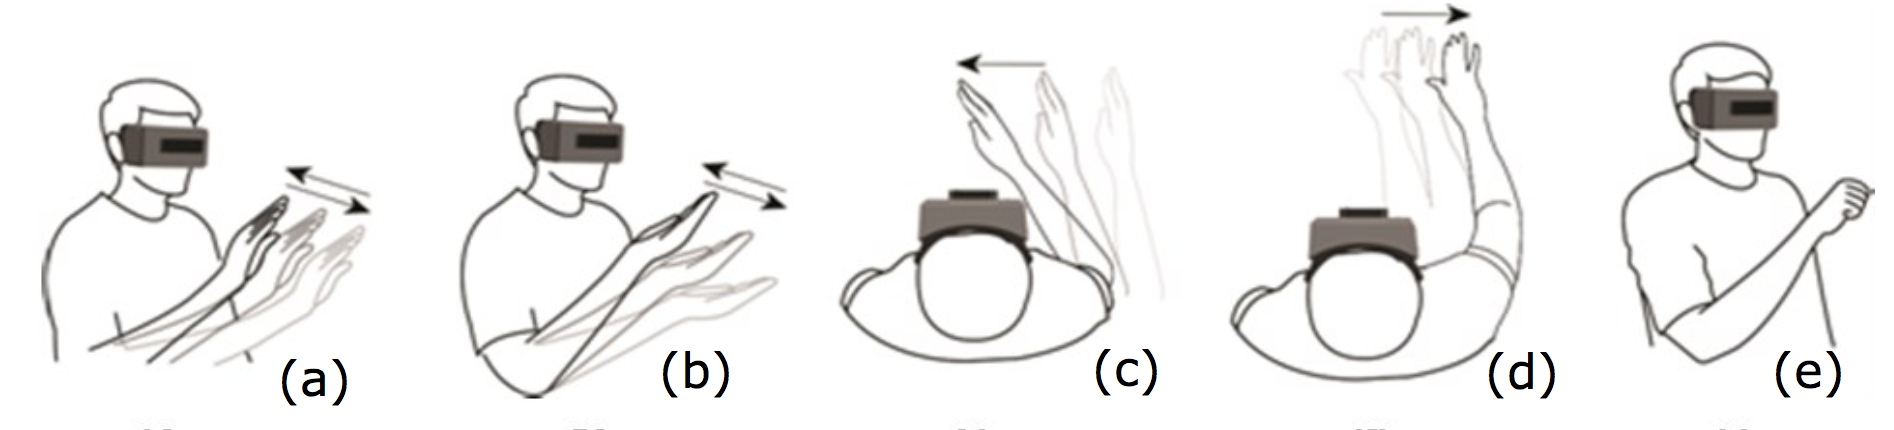
\includegraphics[width=14cm]{03_Figures/05_LitReview/Khundam2015_LeapMotion.png}
		\caption[Hand gestures for forward/backward movement, stepping left/right and holding position]{Hand gestures for forward/backward movement (a,b), stepping left/right (c,d) and holding position (e) \citep{Khundam2015}}
		\label{fig:leapmotion}
	\end{center}
\end{figure}
\newline
For their research on static and stroke gestures, \cite{Chun2015} made use of a depth-camera in order to track hand gestures and combined it with speech recognition. The latter is discussed in more detail in chapter \ref{SubSubSectionSpeechRecognition} which covers the methods of speech recognition in general. \cite{Chun2015} defined different hand and finger gestures for selecting, moving, scaling, rotating, copying and deleting objects, all of which actions had to be confirmed by a specific yes/no gesture. This set of gestures makes it a very natural, intuitive and interactive way for the user to alter virtual objects. As often with the use cameras, there are limitations to it. The hand has to be tracked properly for the whole performance of the gesture and it has to be done with the right speed for a proper recognition of the command \citep{Chun2015}.


\subsubsection{Gesture Controllers}

Very similar to the hand gestures, the gesture controllers intend to improve the tracking of the hand movements by adding hardware to the hands of the users that is easier to track but still leaves options for simple interaction with buttons and triggers. \newline
One of the first commercial gesture controllers was the \textit{PlayStation Move}, introduced by \cite{Sony2010}. While the controller itself can detect its own motion, the position is tracked with a camera attached to the PlayStation. This allows for a more accurate tracking of a specific point which \cite{Takala2014} made use of by attaching a PlayStation Move to their HMD in order to have a more accurate positioning than it was possible with solely the Microsoft Kinect. \newline
Alongside the \textit{HTC Vive} HMD, a new gesture controller also have been introduced \citep{Htcvive2016}. In combination with the Lighthouse technology (described in chapter \ref{360MotionTracking}), the controllers can also be properly tracked if they are e.g. hidden behind the back of the user, which is not possible with the PlayStation Move. Figure \ref{fig:gesturecontroller} shows this controller with its unique design for the tracking sensors (6) and a combination of track-pad (2), buttons (1, 3 and 8) and a trigger (7). By putting the thumb on the track-pad, the index finger on the trigger and the other three fingers on the side button it almost allows to track the grabbing motion of the hand.
\begin{figure}[h]
	\begin{center}
		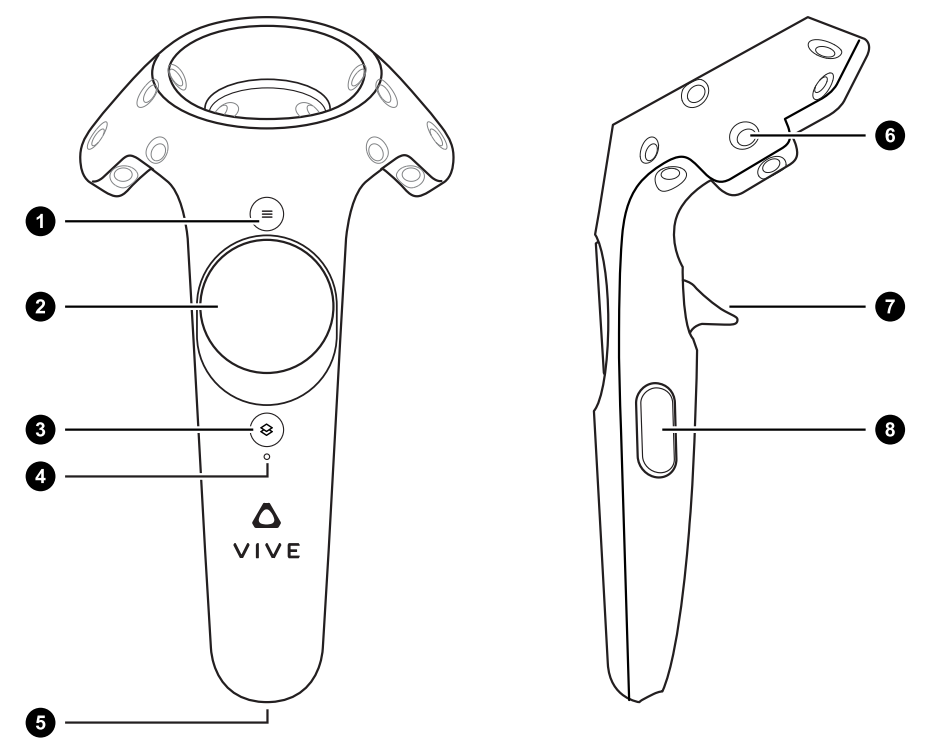
\includegraphics[width=10cm]{03_Figures/05_LitReview/HTCCorp2016_GestureController.png}
		\caption[Gesture Controller for the HTC Vive]{Gesture Controller for the HTC Vive \citep{HTCCorp2016}}
		\label{fig:gesturecontroller}
	\end{center}
\end{figure}


\subsubsection{Speech Recognition}

\label{SubSubSectionSpeechRecognition}

The second natural interaction after hand gestures is speech recognition It is often combined with hand gesture as they can complement each other quite seamlessly. \newline
For the navigation within 3D scans from \gls{mri} or \gls{ct}, \cite{Muller1998} proposed a speech recognition system as illustrated with an example in Figure \ref{fig:speechrecognitionmedical}. With semantic decoding and a semantic structure, the commands can be interpreted and processed by the intention decoder to tell the system what to do \citep{Muller1998}. This is a very time-consuming process since all commands have to be prepared and acoustic-phonetic models need to be generated during the collection of training data. Provided the users followed the instructions, a 99.8\% semantic accuracy could be achieved which basically means that the system is almost fully accurate in this scenario \citep{Muller1998}.
\begin{figure}[h]
	\begin{center}
		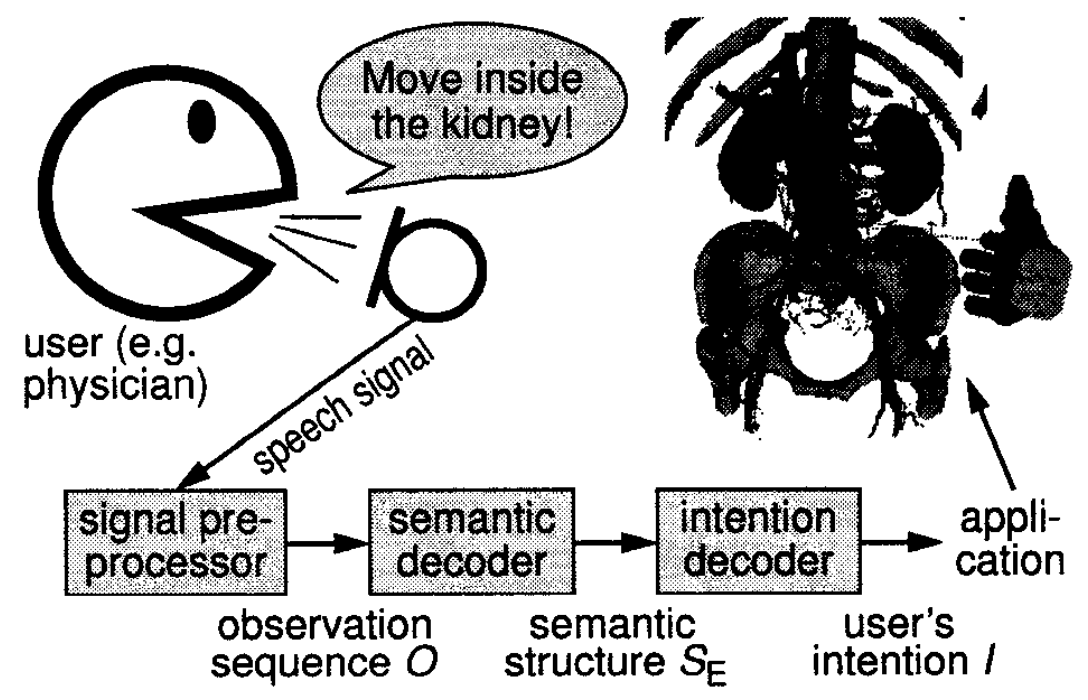
\includegraphics[width=10cm]{03_Figures/05_LitReview/Muller1998_SpeechRecognition.png}
		\caption[Architecture and example of speech recognition and interaction for physicians]{Architecture and example of speech recognition and interaction for physicians \citep{Muller1998}}
		\label{fig:speechrecognitionmedical}
	\end{center}
\end{figure}
\newline
\cite{Uchino2008} combined speech recognition with a camera to identify where the user is pointing at on a computer screen to interact with a virtual agent. In their example, a set of pens with different colours are presented to the user where the selection is made in combination with gestures (pointing at the pen) and speech (e.g. "\textit{Please give the red one}") \citep{Uchino2008}. Figure \ref{fig:speechrecignitionpen} shows how such a conversation with a virtual agent can proceed where the agent picks the wrong pen based on the pointing and ambiguous speech and thus has to be corrected to pick the one with the right colour Although this research was not focussed on virtual reality, this research can also be applied in virtual reality which might even improve the accuracy of the pointing gesture.
\begin{figure}[h]
	\begin{center}
		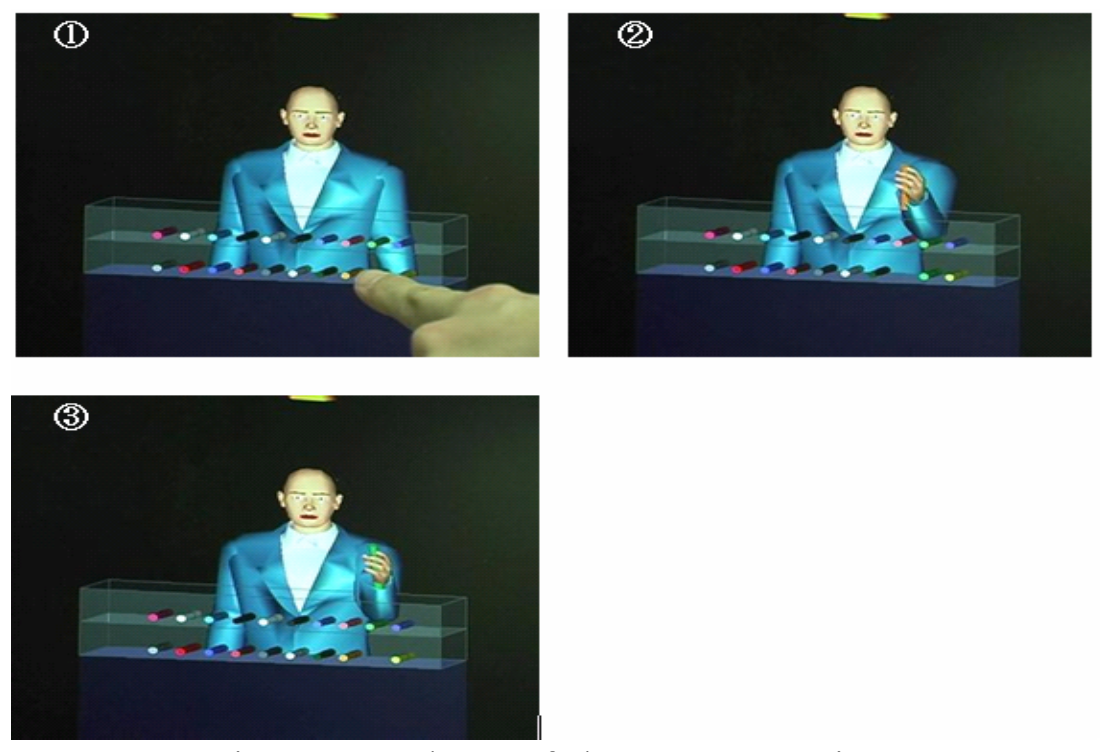
\includegraphics[width=10cm]{03_Figures/05_LitReview/Uchino2008_SpeechPointing.png}
		\caption[Flow of a conversation with the virtual pen agent]{Flow of a conversation with the virtual pen agent \citep{Uchino2008}}
		\label{fig:speechrecignitionpen}
	\end{center}
\end{figure}
\newline
As described in chapter \ref{SubSubSectionHandGestures}, \cite{Chun2015} utilized hand gestures to interact with virtual objects and further enhanced them with speech recognition. While objects can be altered in their spatial appearance, speech is used to change the colour of the object or ask questions about the type, shape or colour of it \citep{Chun2015}. Instead of relying on a physical device with buttons to change the colours, a multi-modal interaction combines speech and gesture to a more natural and intuitive method that is also closer to the real world \citep{Chun2015} .


\subsubsection{Physical Placement of Interactive Objects}

Quite a bit older, from the 1990s, is the idea of dynamically placing physical knobs and switches in front of a seated user wearing a HMD \citep{Latham1997}. The trajectory of the users hand and its movement is extrapolated in order to move the correct type of control in the right position just when it is expected in the virtual reality environment \citep{Latham1997}. Figure \ref{fig:touchcockpit} shows the concept of \cite{Latham1997} as well as how the final design looked like. Since such a machine requires a lot of time to design and build, it can be assumed that these are parts of the reason why not many further advancements were undertaken.
\begin{figure}[h]
	\begin{center}
		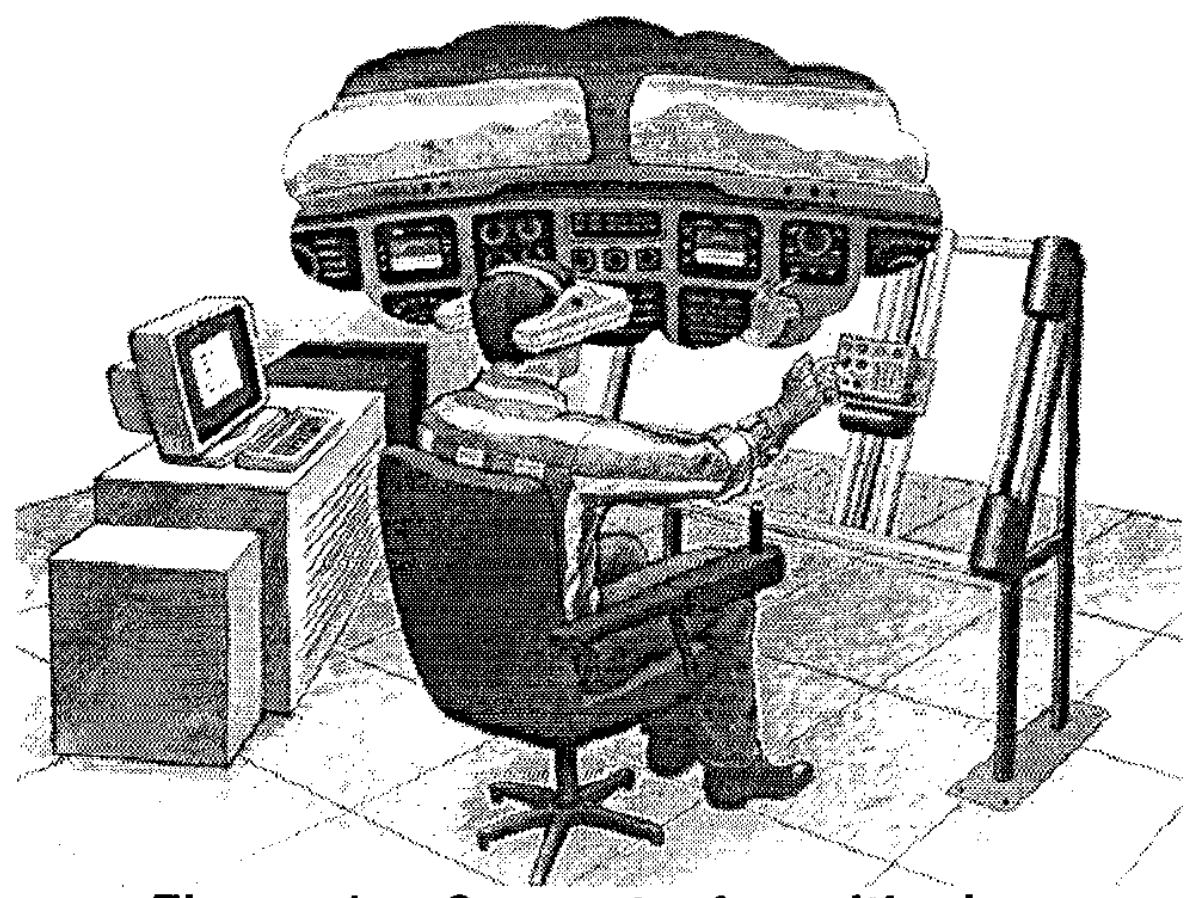
\includegraphics[width=6cm]{03_Figures/05_LitReview/Latham1997_Concept.png}
		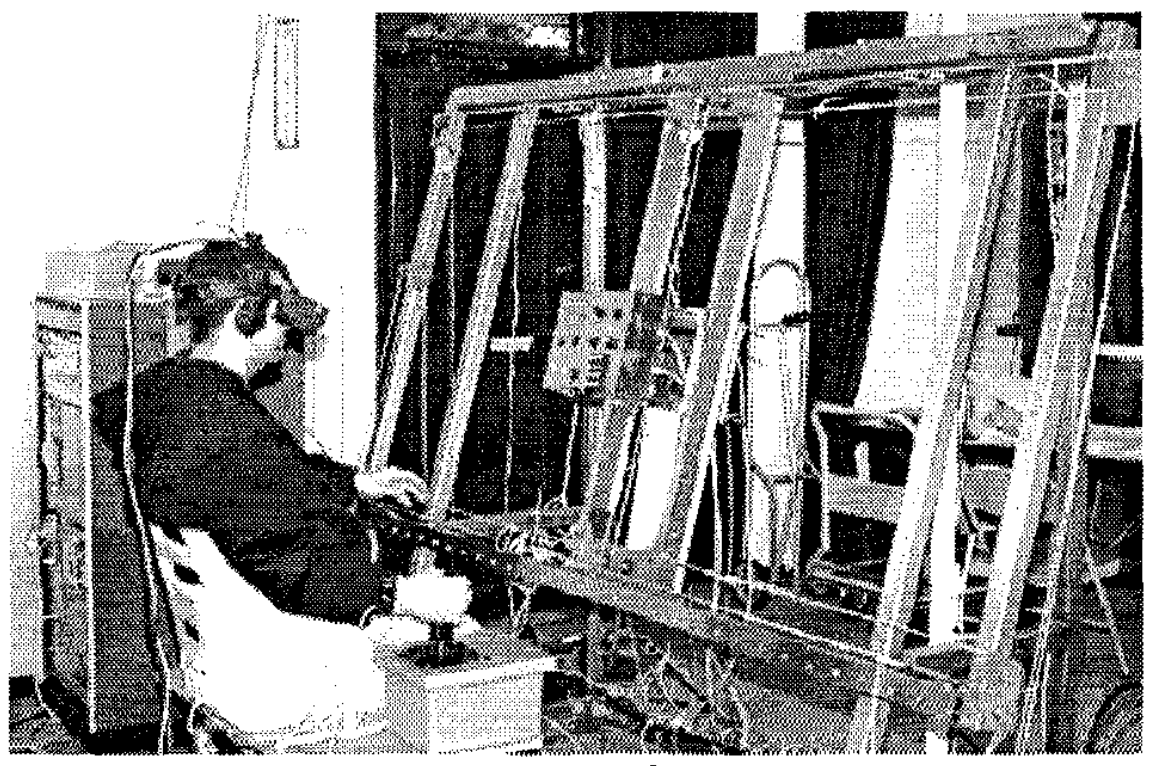
\includegraphics[width=7cm]{03_Figures/05_LitReview/Latham1997_FinalDesign.png}
		\caption[Concept and final design of positioning instrument controls to be touched in a virtual cockpit]{Concept (left) and final design (right) of positioning instrument controls to be touched in a virtual cockpit \citep{Latham1997}}
		\label{fig:touchcockpit}
	\end{center}
\end{figure}


\subsubsection{Full Body Tracking}

In June 2010, Microsoft announced the \textit{Kinect for Xbox 360}, a controller-free gaming device for the living room \citep{Microsoft2010}. Instead of relying on any physical input devices, the Kinect contains a camera with motion-sensing technology that can track up to 48 points of movement on the human body, turning the player himself into a controller \citep{Microsoft2010}. \newline
Based on this technology, \cite{Takala2014} proposed a combination of a full body avatar controlled by Kinect with the Oculus Rift as display. This combination proved to be quite powerful although they were facing a couple of challenges as well. The Kinect sometimes lost track of the hands or the movement was not recognized at all which \cite{Takala2014} tried to resolve by attaching a PlayStation Move to the HMD and put a Razer Hydra controller into the hands (Figure \ref{fig:kinectbody}). Although this improved the situation, different latencies of the individual devices dampened the experience. Furthermore, although Kinect was used for full-body tracking, only the movement of the hands and legs was utilized, whereas the movement within the virtual world was still relying on a physical controller.
\begin{figure}[t]
	\begin{center}
		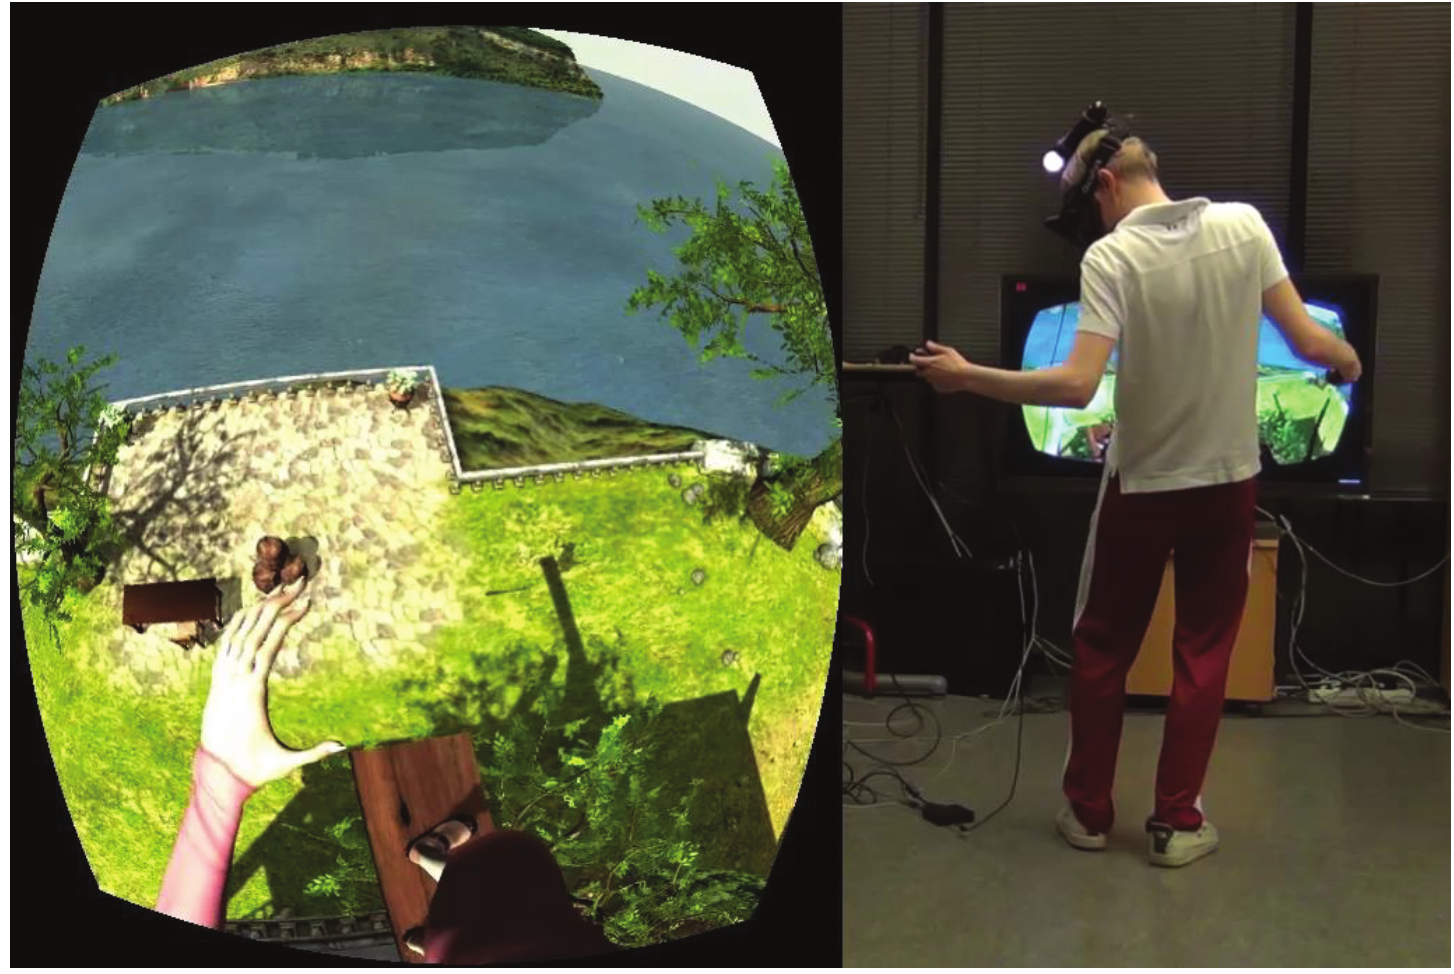
\includegraphics[width=12cm]{03_Figures/05_LitReview/Takala2014_KinectBody.png}
		\caption[Player's view of their virtual body that is tracked with Kinect]{Player's view of their virtual body (left) that is tracked with Kinect (right) \citep{Takala2014}}
		\label{fig:kinectbody}
	\end{center}
\end{figure}


\subsubsection{360° Motion Tracking}
\label{360MotionTracking}

One of the latest additions to the interaction possibilities is the 360° motion tracking, introduced with the HTC Vive which was just released in April 2016 \citep{Htcvive2016}. Figure \ref{fig:lighthouses} shows the setup of the two base stations (i.e. Lighthouses) in opposing corners of the room that will be used for the 360° motion tracking. In essence, the two Lighthouse base stations emit a laser sweep across the room 60 times a second with a flash in between which allows any device with photo-sensors to calculate its exact position relative to the base station(s) \citep{Gizmodo2015}. This allows for a very accurate tracking and due to the opposing corners, at least one Lighthouse always has direct \textit{line of sight} to the HMD and the controllers. \newline
With this additional sensor information, the movement of the HMD and the controllers is tracked in all three axis and allows for new movements to be recognized, such as crouching or jumping within the relations of the room.
\begin{figure}[h]
	\begin{center}
		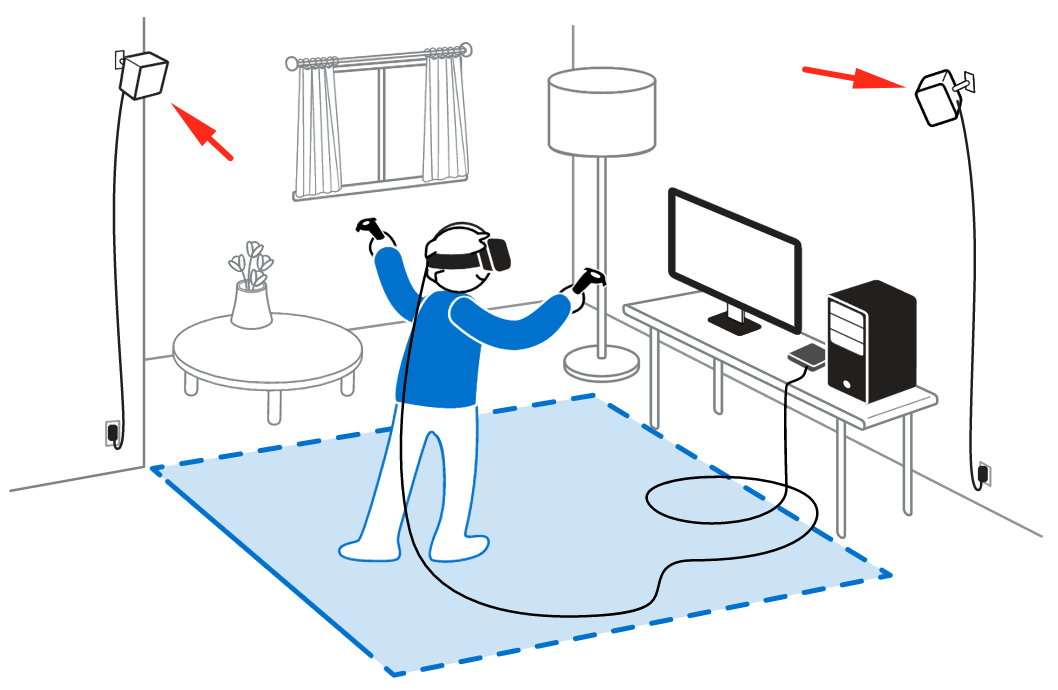
\includegraphics[width=10cm]{03_Figures/05_LitReview/HTCCorp2016_LighthouseRoomScale.png}
		\caption[Two Lighthouse in opposing corners allow for 360° motion tracking]{Two Lighthouse in opposing corners allow for 360° motion tracking \citep{HTCCorp2016}}
		\label{fig:lighthouses}
	\end{center}
\end{figure} \newline
A more simplified variation of this is described by \cite{Donalek2014}, who used a ViconTM motion-capturing system with infrared markers on the HMD to track its spatial location. This allowed \cite{Donalek2014} to also recognize movements such as kneeling down or looking over and around objects in the scene, however always limited by the volume that was covered by the Vicon system. \newline
The main difference to full body tracking is that the 360° motion tracking relies on physical sensors to derive their (i.e. the sensors) position within three dimensional space compared to the detection of any movable object (usually the body of a person). This method is much more accurate than the full body tracking, but requires additional hardware to do so.


%-----------------------------------
%	SUBSECTION 3
%-----------------------------------

\subsection{Conclusion}

The literature review on different methods for user input in virtual reality showed that there are various types which can be used or even combined. \newline
There are six main methods for user input in virtual reality. These are hand gestures, gesture controllers, speech recognition, physical placement of interactive objects, full body tracking and 360° motion tracking. Hand gestures track the movement of the whole hand and/or the individual fingers with one or more (regular, infra-red or depth) cameras. Gesture controllers are physical devices with buttons that are held in the hands and also tracked in their spatial position. Speech recognition tries to understand and interpret spoken words and sentences in order to find the correct commands. The physical placement of interstice objects extrapolates the movement of the hand to physically place a button in front of the finger where a virtual one is shown in \gls{vr}. Full body tracking uses cameras to track the whole body including the movement of all extremities from one angle. Finally, 360° motion tracking can locate the position of special devices within an actual room on all three axis from opposing corners. The most used method in the reviewed literature is the hand gestures, followed by the hand gestures in combination with speech recognition \newline
Depending on the chosen method, there are advantages and disadvantages (or even limitations) for certain use cases. Table \ref{tbl:methodscomparison} shows a summary of these findings and is also the answer to the first \gls{srq}.
\begin{table}[h]
	\begin{center}
		\begin{tabular}{ | p{3.7cm} | p{4.9cm} | p{4.9cm} | } 
			\hline
			\textbf{Method} & \textbf{Advantages} & \textbf{Disadvantages} \\
			\hline
			Hand Gestures & 
			- Highest familiarity \newline - Inexpensive & 
			- Limited tracking area \newline - Only from one angle \newline - Decreasing accuracy with faster movement  \\
			\hline
			Gesture Controllers &
			- Very accurate \newline - Similarity to hand gestures \newline - Buttons for more interaction &
			- Additional device required \newline - Have to be held all the time \\
			\hline
			Speech Recognition &
			- Most natural to humans \newline - Known from smartphones &
			- Different languages, dialects \newline - Requires silent area \\ 
			\hline
			Physical Placement of Objects &
			- Realistic experience \newline - Tangible interaction with \gls{vr} &
			- Expensive \newline - Difficult to build \newline - Stationary \\ 
			\hline
			Full Body Tracking &
			- Tracks all extremities \newline - Natural interaction possible &
			- Only from one angle \newline - Limited accuracy on details \\ 
			\hline
			360° Motion Tracking &
			- Room-scale movement \newline - Very accurate \newline - Spatial positioning on all three axis &
			- Only dedicated HMD and controllers can be tracked \newline - Stationary (base stations) \\ 
			\hline
		\end{tabular}
		\caption{Advantages and disadvantages/limitations of different methods for user input in virtual reality}
		\label{tbl:methodscomparison}
	\end{center}
\end{table} \newline
In regards of the thesis statement, a combination of two methods is recommended to outweigh the individual disadvantages and utilize the benefits of both methods.


%----------------------------------------------------------------------------------------
%	SECTION 2
%----------------------------------------------------------------------------------------

\section{Existing Interaction Patterns in Virtual Reality}

\label{SectionLiteratureReviewSRQ2}

This chapter addresses the second SRQ by having a look at existing interaction patterns in virtual reality and evaluating their strengths and weaknesses. It starts with a short introduction, followed by an analysis of the visual information seeking mantra. Then more details are given on different interaction patterns for travel, selection and manipulation as well as the idea of multi-modal interaction, before the importance of immersion and task performance is elaborated. A conclusion summarises the research done in this chapter.
\begin{framed}
	\textit{SRQ 2: Which ways for interaction with multi-dimensional data exist and what are their strengths and weaknesses?}
\end{framed}

%-----------------------------------
%	SUBSECTION 1
%-----------------------------------

\subsection{Introduction}

During the 1960s, the first interaction patterns such as clicking or grabbing and moving objects have been defined on which even now we are still relying on with mouse and keyboard \citep{Myers1998}. But with wearing a \gls{hmd}, the situation changes as it obstructs our view on the so well known devices. New methods for user input had to be researched and inherently also new interaction patterns had to be defined. \cite{Donalek2014} mentioned that a new tool is required where physical gestures can be used to manipulate with virtual objects. In order to understand what kind of gestures should be considered, the Visual Information Seeking Mantra of \cite{Shneiderman1996} is looked at.


%-----------------------------------
%	SUBSECTION 2
%-----------------------------------

\subsection{Visual Information Seeking Mantra}

\cite{Shneiderman2005} defined a set of principles for direct manipulation, amongst which are:
\begin{itemize}[noitemsep,nolistsep]
	\item visual representation of the world of action including both the objects and actions
	\item rapid, incremental and reversible actions
	\item selection by pointing (instead of typing)
\end{itemize}
Based on this, \cite{Ahlberg1994} proposed the Visual Information Seeking Principle in 1994 that focused in displaying a graph with buttons and sliders for real-time manipulation of the displayed data. This concept fulfilled all principles for direct manipulation and was so successful that it became the foundation for the \gls{vism} \citep{Shneiderman1996}. \cite{Shneiderman1996} was looking at many visual design guidelines but fundamentally always concluded the following mantra:
\begin{framed}
	\textit{Overview first, zoom and filter, then details-on-demand}
\end{framed}
As an abstraction of reality, \cite{Shneiderman1996} further defined seven tasks (four main and three support tasks) that are inherently crucial for the analysis and work with data.

Main tasks:
\begin{itemize}[noitemsep,nolistsep]
	\item Overview \textit{(Gain an overview of the entire collection)}
	\item Zoom \textit{(Zoom in on items of interest)}
	\item Filter \textit{(Filter out uninteresting items)}
	\item Details-on-demand \textit{(Select and item or group and get details when needed)}
\end{itemize}
Support tasks:
\begin{itemize}[noitemsep,nolistsep]
	\item Relate \textit{(View relationships among items)}
	\item History \textit{(Keep a history of actions to support undo, replace and refinement)}
	\item Extract \textit{(Allow extraction of sub-collections and of the query parameters)}
\end{itemize}
Figure \ref{fig:vism} shows a visualisation of these tasks as well as the relationship to each other. It shows that in order to move from the \textit{Overview} to the \textit{Details}, the user either has to \textit{Zoom} or apply some \textit{Filtering} on the presented data set.
\begin{figure}[h!]
	\begin{center}
		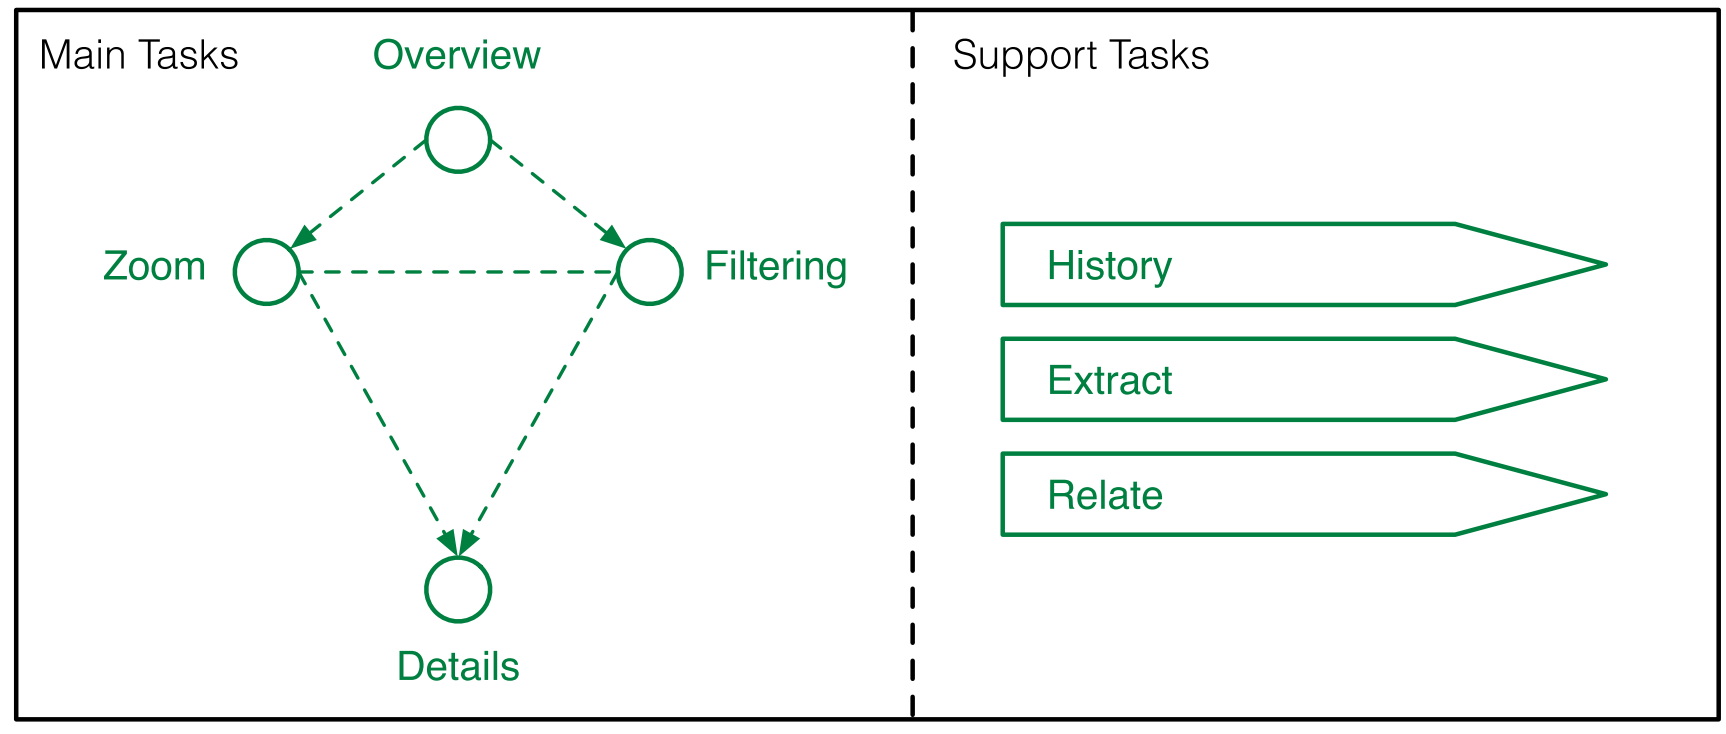
\includegraphics[width=12cm]{03_Figures/05_LitReview/Stauffer2016_VISM1.png}
		\caption[Visual Information Seeking Mantra]{Visual Information Seeking Mantra \citep{Stauffer2016}}
		\label{fig:vism}
	\end{center}
\end{figure} \newline
\cite{Stauffer2016} reviewed and extended the \gls{vism} to version 2.0. By distinguishing between \textit{Zoom In} and \textit{Zoom Out} as well as allowing for a more flexible entry point for the different tasks, they also deal with one of the big downfalls of \gls{vism} when a user already knows what data is important and thus does not want to start with the \textit{Overview} \citep{Neil2006}. Shifting \textit{Relate} to the main tasks helps to align it with \textit{Details} to provide a multi view where multiples views can be shown and altered simultaneously \citep{Stauffer2016}. The additional \textit{Collaboration} support tasks suggest that communication possibilities should be implemented directly inside the the application system instead of relying on third party applications. Figure \ref{fig:vism2} shows version 2.0 of the \gls{vism} with a direct comparison of 1.0 (green) and 2.0 (orange). \newline
\begin{figure}[h!]
	\begin{center}
		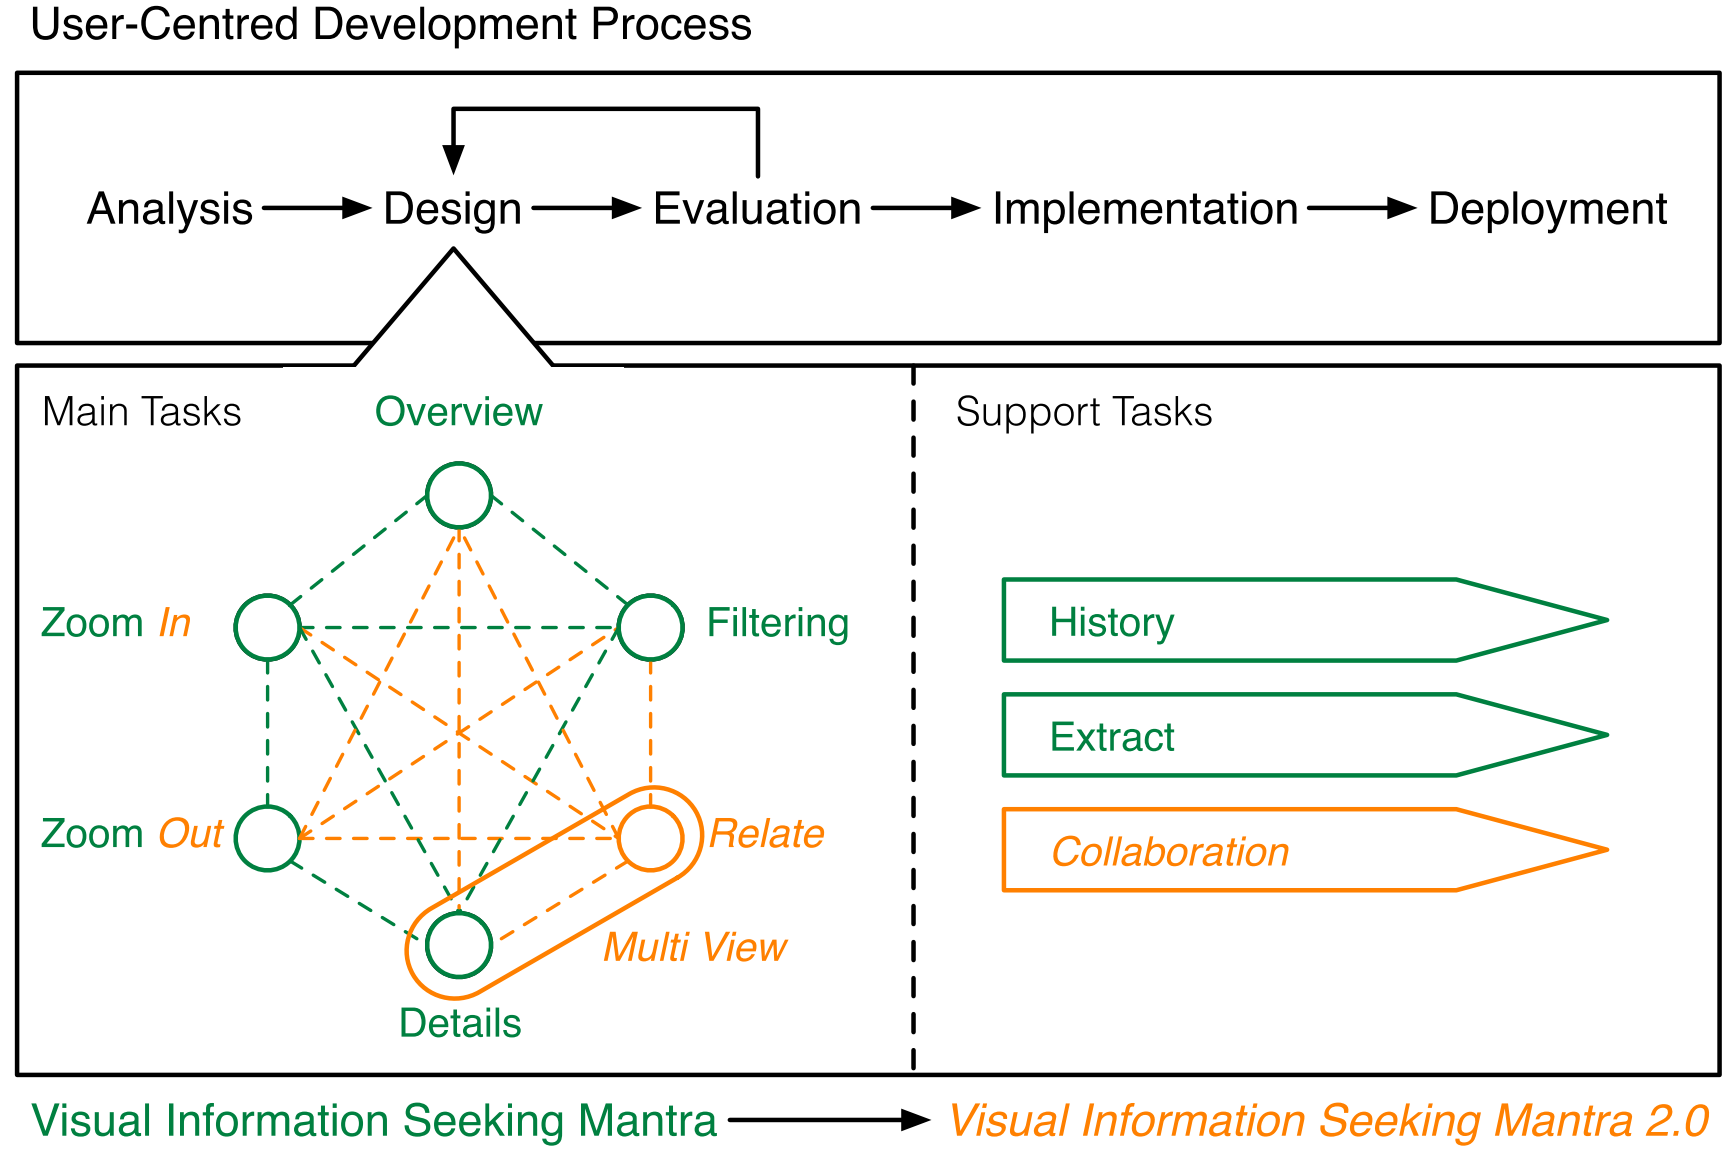
\includegraphics[width=12cm]{03_Figures/05_LitReview/Stauffer2016_VISM2.png}
		\caption[Visual Information Seeking Mantra 2.0]{Visual Information Seeking Mantra 2.0 \citep{Stauffer2016}}
		\label{fig:vism2}
	\end{center}
\end{figure}

In the analysis of \gls{vism} by \cite{Craft2005}, they point out that it should only be seen as guidelines and also note that although it defines some tasks that a system \textit{should} fulfil, it gives no indication on the question \textit{"How?"}. This conclusion can still be seen as valid since also with version 2.0 of the \gls{vism}, the focus remains on what kind of interaction should be present and not how these interactions could look like.


%-----------------------------------
%	SUBSECTION 3
%-----------------------------------

\subsection{Interaction Patterns}

\cite{Bunt1998} stated that "Human communication is inherently multimodal in nature". What he meant with this is that in a multi-modal user interface, a user can combine a spoken natural language request with one or more gestures \citep{Rosson2002}. By allowing this combination, the interaction in virtual reality can become closer to how we already interact with each other in real life. \newline
In order to understand the different interaction patterns better, \cite{Bowman2002} has grouped them in three distinctive categories: Travel, Selection and Manipulation. \textit{Travel} deals with how the user can navigate in the virtual environment, how the movement and visual exploration works. \textit{Selection} focuses on the first interaction with a virtual object, how one or many object can be selected and how this is visualised for the user. Finally, in \textit{Manipulation} the actual alteration of a virtual object in its appearance and behaviour is discussed.


%-----------------------------------
%	SUBSUBSECTION 1
%-----------------------------------

\subsubsection{Travel}

In \gls{vr}, the most important interaction pattern is the navigation itself, since without navigation the experience is not much different from a 2D display. \cite{Kwon2015} and \cite{Jamieson2007} confirmed in their research that the simplest method for this is to utilize the built in head tracking capabilities of the \gls{hmd} itself. It in fact is more familiar to us humans to examine objects of interest this way, rather than using mouse and keyboard \citep{Jamieson2007}. Either with the gyroscope sensor information or with tracking the position and direction of the camera, this information allows to determine where the user is looking at \citep{Kwon2015}. \cite{Jamieson2007} continue that for a totally immersive experience in \gls{vr}, also body movement would have to be tracked to allow to walk around or even to put the head inside the visualised data objects.

\cite{Deligiannidis2003} researched this topic based on a problem from practice where a person is working on a specific task in \gls{vr} and up to 20 outsider participants can observe and comment on the work of the fully immersed person. The use of vocal instructions however was distracting to everyone and there were no possibilities for the outsiders to interact with the virtual environment \citep{Deligiannidis2003}. Their solution to this was dividing the area in front of each outsider into two hemispheres, reaching with the hands in the top one allowed each person to manipulate the camera (third person view) whereas if the hands are on the lower one the hand manipulation (first person view) was activated \citep{Deligiannidis2003}. This combination allowed the before passive observers to be much more immersed in the virtual environment and to do exploration on their own.

During their demonstrations, \cite{Drouhard2015} observed difficulties when the users wearing a \gls{hmd} had to interact (blindly) with keyboard and mouse, whereas most of them could use an Xbox controller rather intuitively. In their application, the controller was used to "fly" around within the virtual environment and the head tracking capabilities of the \gls{hmd} allowed them to explore the environment and look at the data from different perspectives \citep{Drouhard2015}.

\cite{Bowman2002} also defined guidelines for designing travel techniques, which inherently are related to the navigation and can be summarized as follows:
\begin{itemize}[noitemsep,nolistsep]
	\item Make simple travel tasks simple by using target-based techniques
	\item Use physical head motion for viewpoint orientation if possible
	\item Avoid teleportation; provide smooth transitional motion between locations instead
	\item If steering techniques are used, users should be trained beforehand
	\item Use non-head-coupled techniques for efficiency in relative motion tasks
	\item Provide integrated aids to help the user decide where to move
\end{itemize}

The reviewed literature showed that for looking around, researchers exclusively relied on the head-tracking capabilities of the \gls{hmd} whereas for the travel in space either third-party controllers were used or the idea of full body tracking was briefly mentioned.

On a more practical side, \cite{CloudheadGames2016} released their \gls{vr} game \textit{The Gallery - Episode 1: Call of the Starseed} for the HTC Vive in April 2016 and offered two different ways for travelling in the virtual environment. The player can chose between "gaze-teleportation" where the location to be teleported at is controlled with the \gls{hmd} and confirmed with a click, or "point-teleportation" where the target spot is chosen and confirmed by pointing at with the gesture controller \citep{CloudheadGames2016}. While the travelling with gaze follows the research of \cite{Jamieson2007} and their conclusion that using the \gls{hmd} is the simplest method, it limits the possibilities for multitasking. By utilizing the gesture controllers for travelling, a certain independence of the viewing experience is achieved and allows "blind" travelling without the need to also look into that direction, just like if we walk backwards in the real world. Both methods of travelling are illustrated in Figure \ref{fig:gazePointTeleportation}.
\begin{figure}[h]
	\begin{center}
		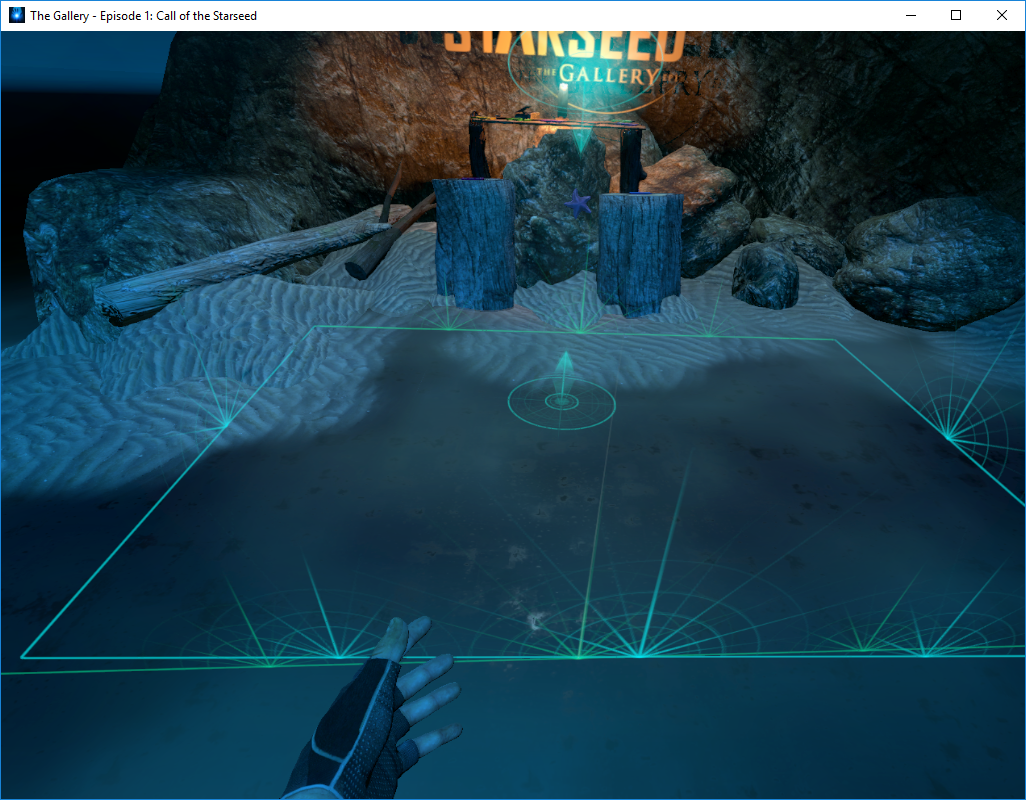
\includegraphics[width=7cm]{03_Figures/05_LitReview/Cloudhead2016_TheGallery2.png}
		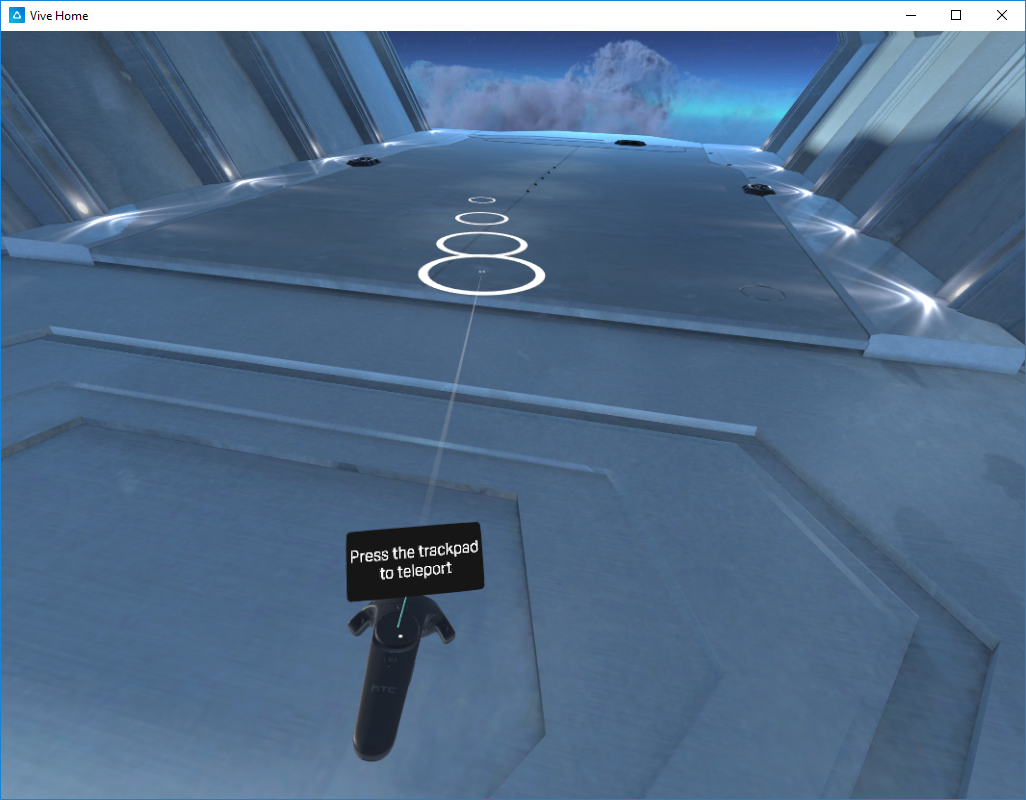
\includegraphics[width=7cm]{03_Figures/05_LitReview/HTCVive2016_ViveHome.png}
		\caption[Gaze and point teleportation in "The Gallery" and "Vive Home"]{Gaze (left) and point (right) teleportation in "The Gallery"  \citep{CloudheadGames2016} and "Vive Home" \citep{Htcvive2016a}}
		\label{fig:gazePointTeleportation}
	\end{center}
\end{figure} \newline
The fact that both options are provided for the player to chose from can be seen as an indication, that even in practice for entertainment purposes, there is no clear strategy yet as to which travelling method is more natural, efficient or practical.

%-----------------------------------
%	SUBSUBSECTION 2
%-----------------------------------

\subsubsection{Selection}

After looking at \textit{Travel}, the second interaction pattern is the selection of objects in the virtual environment either to get more information on them or to do manipulate them in a subsequent step. Based on the selected input method, different patterns come to action. \newline
\cite{Bowman2002} also defined guidelines for designing selection techniques that can be summarised as follow:
\begin{itemize}[noitemsep,nolistsep]
	\item Use the natural virtual hand technique if all selection is within arm's reach
	\item Use ray-casting techniques if speed of remote selection is a requirement
	\item The chosen selection technique should integrates well with the manipulation technique
	\item Multi-modal input for combined selection and command tasks
	\item Environment design should maximize the perceived size of objects
	\item Provide integrated aids to help the user decide where to move
\end{itemize}

Research showed, that three main types of selection patterns have been research: Hand, HMD Reticle and Gesture Controllers.

\subparagraph{Hand}

\cite{Steed2006} researched different simple selection techniques using the hand. He distinguishes between Ray-based selection, Small Volume Selection and Cone Selection which are illustrated in Figure \ref{fig:selectiontechniques} \citep{Steed2006}. In the Ray-based selection, an imaginary ray is cast in the direction of the hand to choose the first object interacts with (object A), whereas in the Small Volume selection, the intersection of the hand with the volume of an object determines the selection (object C) \citep{Steed2006}. Lastly, \cite{Steed2006} defined the Cone Selection similar to the Ray-based one, however there are two rays in this case and all objects that are in between them are considered selected (objects E and F). \newline
Each technique has different applications where it makes more sense or allows for a better immersion than any of the other techniques, such as when a virtual button or handle can be triggered, the Small Volume selection can be considered the closest to how we would interact in the real world. \newline
Since these techniques are highly linked to the methods of using hand gestures as input, they bring their strengths and weaknesses along. While it is the most familiar way for humans to interact (or in this case to select something), it is highly depending on accurate tracking capabilities and good interpretation of gestures if more than a simple pointing gesture is required.
\begin{figure}[h]
	\begin{center}
		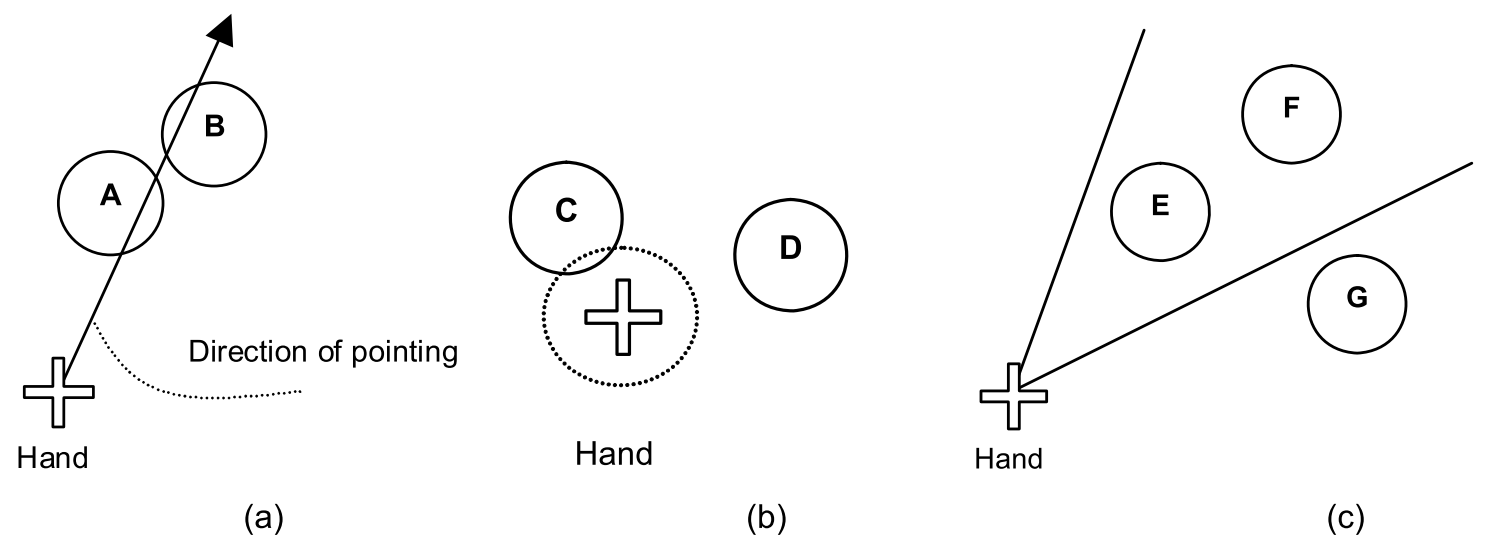
\includegraphics[width=14cm]{03_Figures/05_LitReview/Steed2006_SelectionTechniques.png}
		\caption[Simple selection techniques for objects in VR: Ray-based, Small Volume Selection and Cone Selection]{Simple selection techniques for objects in VR: Ray-based (a), Small Volume Selection (b) and Cone Selection (c) \citep{Steed2006}}
		\label{fig:selectiontechniques}
	\end{center}
\end{figure}


\subparagraph{HMD Reticle}

\cite{Kwon2015} and \cite{Drouhard2015} focused their research on a selection technique using a reticle that is visualised inside the \gls{hmd}, like a cross-hair. When the user selects a node with this reticle, this node and its neighbours are brought closer to the user and are highlighted in order to see more details and allow the user to make further selections \citep{Kwon2015}. With the option to select multiple nodes and the visualization of the nodes amongst themselves, interesting paths or relations can be visualized in an effective way \citep{Kwon2015}. It however is not mentioned how the selection itself is triggered, whether a button has to be pushed or if the gaze just has to be held for a couple of seconds. It is also not mentioned how the "\textit{Zoom Out}" task can be performed. \newline
\cite{Drouhard2015} provided more details on this part in their research where they implement a "target mode" that the user can enter. Only in this case the cross-hair reticle is shown to the user and the selection happens by targeting a data object and pressing the trigger button \citep{Drouhard2015}. It can be assumed that this separation of "target mode" and "view mode" will help the combination of \textit{Selection} and \textit{Travel} and makes the data analysis more convenient as the reticle is only shown when absolutely necessary. \newline
\cite{Drouhard2015} furthermore states that gaze interaction arguably is the most natural form of interaction in virtual environments. \newline
One fact that is not mentioned in literature but becomes clear is that with an \gls{hmd} reticle, the selection is directly linked to the viewing experience. It is not possible to select something without directly looking at it, which inherently limits the multitasking possibilities.


\subparagraph{Gesture Controller}

Finally, also gesture controllers allow for dedicated selection patterns. \cite{Hentschel2009} used a controller to select multiple data points out of a 3D scatter-plot which they called interactive brushing and is shown in Figure \ref{fig:interactivebrushing}. The first (left) picture shows the empty selection box that can be moved and scaled (middle and right picture) in order to make the actual selection \citep{Hentschel2009}. Although the middle and right picture look almost the same, the difference is that with the middle picture the visualization of the scatter-plot is done in real-time and only upon releasing the button on the device, the actual selection with remote selection and computing is done \citep{Hentschel2009}.
\begin{figure}[h]
	\begin{center}
		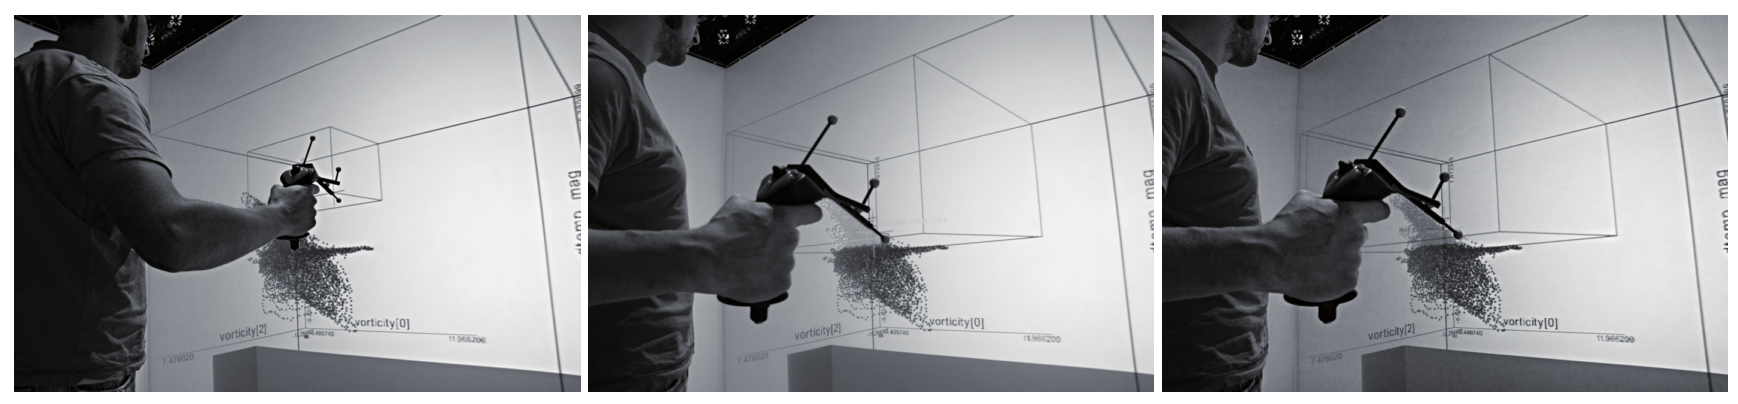
\includegraphics[width=14cm]{03_Figures/05_LitReview/Hentschel2009_InteractiveBrushing.png}
		\caption[Box selection of scatter-plot data in VR]{Box selection of scatter-plot data in VR \citep{Hentschel2009}}
		\label{fig:interactivebrushing}
	\end{center}
\end{figure} \newline
In their game \textit{The Gallery - Episode 1: Call of the Starseed}, \cite{CloudheadGames2016} provide the option to select objects by utilizing the gesture controllers that in \gls{vr} are visualised as hands as shown in Figure \ref{fig:theGalleryHands}. With the trigger button, the hand can be closed and thus objects can be grabbed and moved around. The game further distinguishes between "important" and "unimportant" objects, where the "important" ones are stuck in the grip of the hand even if the trigger was released (i.e. a flashlight) and "unimportant" objects would immediately drop once the trigger button is released. This allows for a more convenient interaction since it can become irritating to keep the trigger button held for a longer amount of time. \newline
\begin{figure}[h]
	\begin{center}
		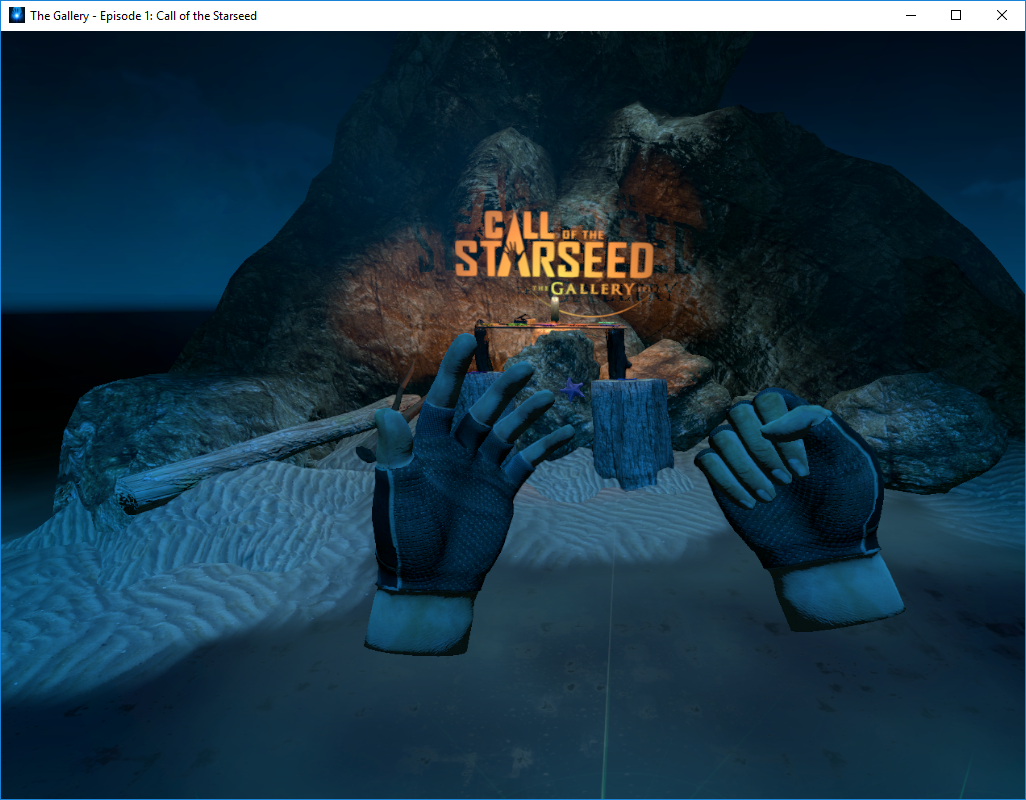
\includegraphics[width=7cm]{03_Figures/05_LitReview/Cloudhead2016_TheGallery.png}
		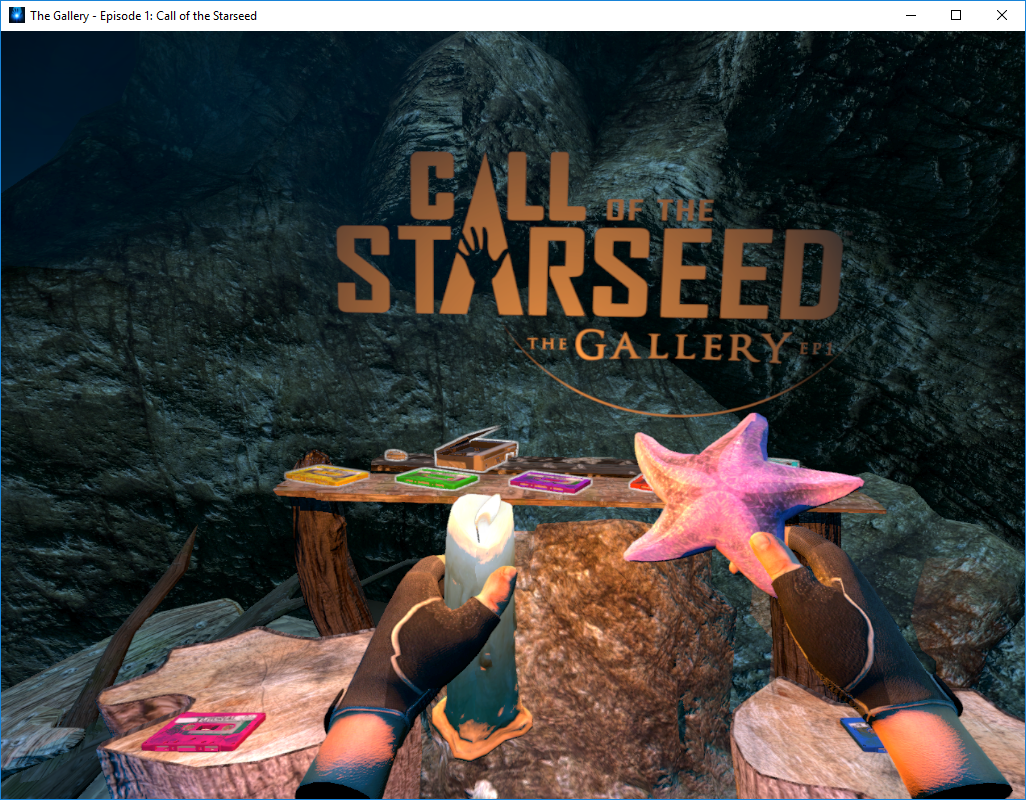
\includegraphics[width=7cm]{03_Figures/05_LitReview/Cloudhead2016_TheGallery3.png}
		\caption[Gesture Controllers visualized as Hands in "The Gallery"]{Gesture Controllers visualized as Hands in "The Gallery" \citep{CloudheadGames2016}}
		\label{fig:theGalleryHands}
	\end{center}
\end{figure} \newline
As with the selection by hand, also the selection by gesture controllers brings their advantages and disadvantages from the method as an input device itself with them. While they offer very good accuracy and increased functionality with buttons and triggers, it requires additional hardware and tracking devices.


%-----------------------------------
%	SUBSUBSECTION 3
%-----------------------------------

\subsubsection{Manipulation}

As early as in the 1980s, interaction patterns with data (i.e. manipulations) have already been defined, such as the "Put-That-There" voice and gesture interface as described by \cite{Bolt1980}. This interfaces focus on certain voice command to manipulate objects in a virtual space which have been defined as following \citep{Bolt1980}:
\begin{itemize}[noitemsep,nolistsep]
	\item "Create..." \textit{(a default object, with default size and colour on a default position)}
	\item "Move..." \textit{(an object to a specific position)}
	\item "Make that..." \textit{(altering an object in colour and size)}
	\item "Delete..." \textit{(removal of an object)}
	\item "Call that..." \textit{(give an object a name to which it can be referred to)}
\end{itemize}
In addition, the spoken \textit{"there"} serves as some kind of voice button where the \textit{"there"} refers to the cursor position, thus introducing the gestures as an input method for this interface \citep{Bolt1980}.
It can be seen that even more than three decades ago, the need to simplify more complicated interactions such as changing the colour of an object, which would require several inputs actions with mouse or keyboard, were tested to be simplified with new means of interaction patterns. \cite{Donalek2014} also mentioned the need for a new tool where the user can manipulate with these objects since wearing a \gls{hmd} blocks the view on the keyboard interface. \newline
\cite{Woodard2015} explained their approach on a more technical level in which they basically utilized the concept of the Small Volume Selection from \cite{Steed2006} to trigger certain manipulations like opening a door (i.e. rotating an object on its axis).

\cite{Bowman2002} again defined guidelines for designing manipulation techniques, that can be summarized as follow:
\begin{itemize}[noitemsep,nolistsep]
	\item Provide constraints (general or specific) or manipulation aids
	\item Allow direct manipulation with the virtual hand instead of using a tool
	\item Avoid repeated, frequent scaling of the user or environment
	\item Use indirect depth manipulation for increased efficiency and accuracy
\end{itemize}

Literature review has shown that most research focuses on \textit{Travel} and \textit{Selection} whereas \textit{Manipulation} of data objects is in most cases not covered at all. This is also shown with the defined guidelines from \cite{Bowman2002} as they are more vague than for the other techniques.

With the release of the HTC Vive, \cite{Google2016} released a \gls{vr} application called \textit{Tilt Brush} which basically is a 3D painting application in virtual reality. It allows the user to choose between different pencils, brush sizes, colours and also provides an "undo" functionality, all that is controlled with pop-up menus that can be interacted with using the gesture controllers as shown in Figure \ref{fig:tiltBrushMenus}.
\begin{figure}[h]
	\begin{center}
		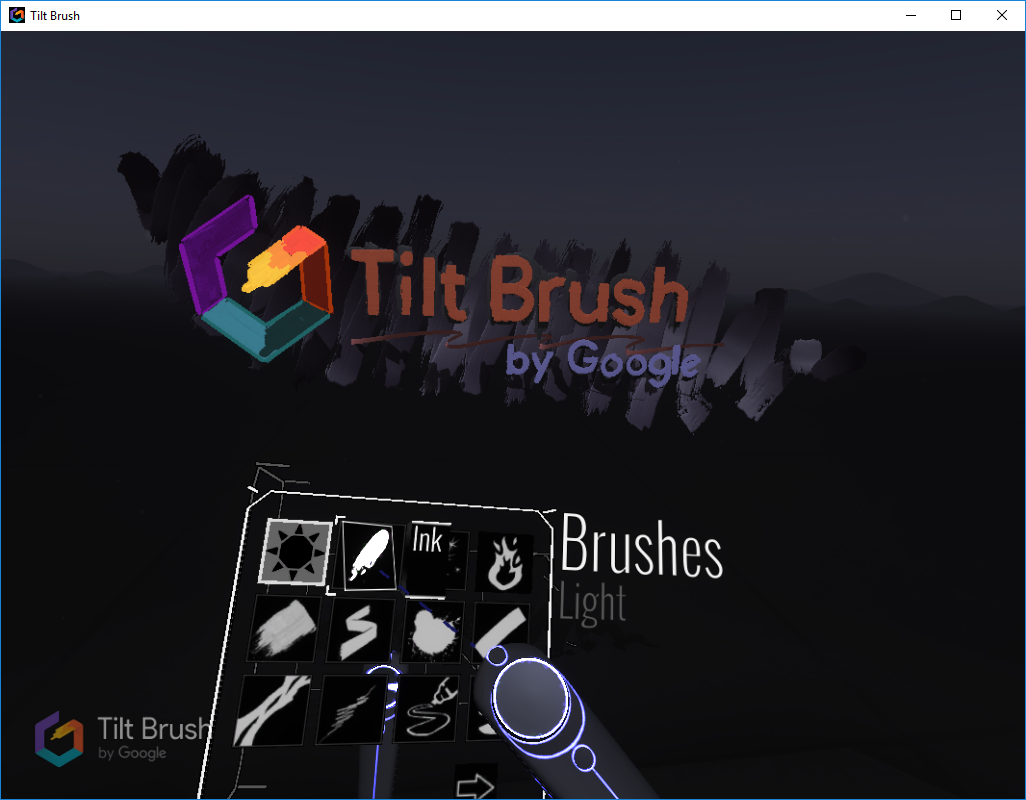
\includegraphics[width=7cm]{03_Figures/05_LitReview/Google2016_TiltBrush.png}
		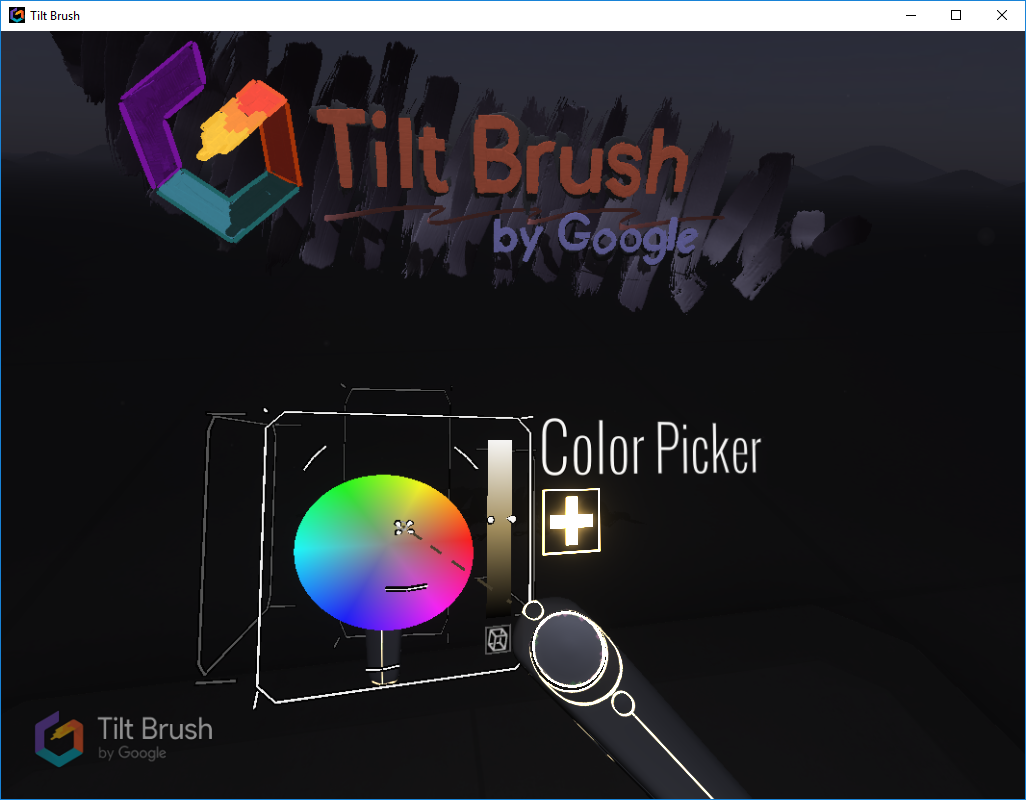
\includegraphics[width=7cm]{03_Figures/05_LitReview/Google2016_TiltBrush2.png}
		\caption[Pop-up menu with Gesture Controllers in "Tilt Brush"]{Pop-up menu with Gesture Controllers in "Tilt Brush" \citep{Google2016}}
		\label{fig:tiltBrushMenus}
	\end{center}
\end{figure} \newline
The research of \cite{Bowman2002} has shown, that although this type of non-natural interaction indeed can be quite effective, especially since it allows for tasks to be executed that cannot be done naturally. Although it would be possible to provide a virtual colour palette where the user would have to choose the colour by hand to eliminate this option from the pop-up menu, this would drastically impact the task performance in a negative way.


%-----------------------------------
%	SUBSECTION 4
%-----------------------------------

\subsection{Importance of Immersion and Task Performance}

In addition to the interaction patterns to perform tasks, the level of immersion and the performance of task execution is as important. \cite{Woodard2015} defined three rules a project has to be conform with in order to be as immersive as possible:
\begin{itemize}[noitemsep,nolistsep]
	\item Three Dimensional Viewing
	\item Full User-Navigation Integration
	\item Interactive Environment
\end{itemize}
The first two points have to be ensured by the application design itself as well as interaction patterns for \textit{Travel}. The third point is more complex as it covers the interaction patterns for \textit{Selection} and \textit{Manipulation} which are more crucial for the performance.

\cite{Bowman2002} separates the term performance a bit more and considers two aspects of it:
\begin{itemize}[noitemsep,nolistsep]
	\item Task performance \textit{(quality of task completion, measured in time, accuracy, ...)}
	\item Technique performance \textit{(qualitative experience of the user during interaction)}
\end{itemize}
Since the technique performance is ultimately related to the concept of usability, which is not part of this thesis, the main focus lies on the task performance.

\cite{Bowman2002} continues that it is a common misconception that in order to be an effective virtual environment, it should behave and work as close to the real world as possible; interaction should be "natural". \cite{Smith1987} called this naturalistic approach "\textit{Naturalism}" whereas the addition of non-natural methods he simply called "\textit{Magic}". The possibility to scale objects or create them out of thin air, to be able to fly around in space are considered to be magic techniques \citep{Bowman2002}. There are also more simple 2D objects such as drop-downs, pop-up menus or buttons that are already widely spread in our everyday applications that we use on computers and smartphones. \cite{Bowman2002} concludes that although these techniques are less natural and might even require some training, if designed for specific interaction tasks, they can be more efficient and flexible than any natural technique.\newline
\cite{Rosson2002} looked at immersion a bit different and summarized it as an "all around" experience for the user which requires multi-modal input (e.g. data gloves or speech recognition) and output (e.g. \gls{hmd} or haptic feedback on a device). The degree to which someone fells like actually being "in" this virtual environment is depending on the available inputs and outputs and is often referred to as presence \citep{Rosson2002}.\newline
It can be said that if a task feels tedious and difficult to execute in \gls{vr}, it will have a difficult time to keep people interested in it, after all it should help us to become more efficient in our task performance.


%-----------------------------------
%	SUBSECTION 6
%-----------------------------------

\subsection{Conclusion}

The \gls{vism} provides a solid foundation of what tasks the interaction patterns should be able to fulfil. It however gives no guidelines or recommendations in how these interaction patterns could look like. The interaction patterns can be grouped into three categories: \textit{Travel}, \textit{Selection} and \textit{Manipulation}. Each of them has its own patterns which are more or less suited for certain applications. In general it can be seen that the \textit{Manipulation} pattern are researched the least so far and can be a suitable candidate for further research. Whichever interaction pattern is selected and implemented, its ability to allow the user to have a good task performance is crucial for any practical applications. \newline
In general, the strengths and weaknesses of the individual patterns are heavily related to advantages and disadvantages of the input method they base on. It can be said that the interaction patterns have to be selected in correlation with the decision for the matching input methods. Table \ref{tbl:pattermethodmapping} shows a mapping of pattern and method.
\begin{table}[t]
	\begin{center}
		\begin{tabular}{ | p{4cm} | p{6cm} | } 
			\hline
			\textbf{Interaction Pattern} & \textbf{Input Method} \\
			\hline
			Travel:  \newline \textit{Controllers} &
			- Gesture Controllers \newline - Physical Placement of Objects \\
			\hline
			Travel: \newline \textit{Full body tracking} &
			- Fully Body Tracking \newline - 360° Motion Tracking \\
			\hline
			Selection: \newline \textit{Hand} & 
			- Hand Gestures \\
			\hline
			Selection: \newline \textit{HMD Reticle} &
			- \gls{hmd} \\
			\hline
			Selection: \newline \textit{Gesture Controllers} &
			- Gesture Controllers \\ 
			\hline
			Manipulation: \newline \textit{"Put that there"} &
			- Speech Recognition \newline - Hand Gestures \\ 
			\hline
			Manipulation: \newline \textit{Others} &
			- Gesture Controllers \\ 
			\hline
		\end{tabular}
		\caption{Mapping of interaction pattern with their correlating input method}
		\label{tbl:pattermethodmapping}
	\end{center}
\end{table}

Although no distinct answer can be given to the second \gls{srq}, in combination with the findings from the first /gls{srq} it has been shown where the strengths lie and how they can be utilized. This also shows the close connection between the input method and interaction pattern and that they have to be aligned in order to create an immersive and productive experience.


%----------------------------------------------------------------------------------------
%	SECTION 3
%----------------------------------------------------------------------------------------

\section{Data Visualization}

\label{SectionLiteratureReviewSRQ3}

After covering the different methods for user input in \gls{vr} in chapter \ref{SectionLiteratureReviewSRQ1} and the interaction patterns in \gls{vr} in chapter \ref{SectionLiteratureReviewSRQ2}, this chapter concludes the literature research by looking at traditional data visualisation that are used for 2D data and how they have been applied to and enhanced for 3D space in \gls{vr}. After a short introduction to the topic, the two main parts of data visualisation and data manipulation are discussed in more detail, with a focus on the differences between the application in 2D respectively 3D space. Finally, the research covered in this chapter is summarized in the conclusion and will answer the third \gls{srq}.
\begin{framed}
	\textit{SRQ 3: Which traditional strategies for visualization and manipulation of 2D data have been applied and enhanced for 3D space in virtual reality?}
\end{framed}


%-----------------------------------
%	SUBSECTION 1
%-----------------------------------

\subsection{Introduction}

With the invention of (multiple) windows on a computer screen in the late 1960s and the first spreadsheet (VisiCalc) developed in the late 1970s, the era for the visualization of data had just begun \citep{Myers1998}. Although the first \gls{hmd} was already invented in 1960 by Morton Heilig, it was only used for non-interactive film without any motion tracking \citep{vrs2015}. The actual availability for the public of such devices was not possible until the early 1990s although they still were rather expensive or did not fulfil the consumers expectations rendering them a flow (e.g. Nintendo Virtual Boy) \citep{vrs2015}. \cite{Ribarsky1994} highlighted that complicated manipulations of data will be simplified as \gls{vr} can provide a more natural interface between human and computer. He further continues that with \gls{vr} more of our senses are engaged than with regular 2D displays and thus can provide an opportunity to combine them \citep{Ribarsky1994}. \cite{Jamieson2007} further confirm the increased effectiveness and more natural and intuitive view on objects that use a 3D approach as it represents how humans view objects. \newline
\citet[p.411]{Stone1994} emphasized that: \blockquote{Visualization is more of a technique than a task. That is, people don't usually visualize data just for the hell of it.} They further conclude that due to the different goals for the visualization (e.g. testing a theory or understanding the data set), it makes it difficult on a general level to discuss the problems with how the visualization should be supported \citep{Stone1994}. This highlights the importance of the right type of visualization depending on the data itself and the goal that shall be reached. For a better understanding, the following chapter will focus on different approaches and techniques for the presentation of data.


%-----------------------------------
%	SUBSECTION 2
%-----------------------------------

\subsection{Data Presentation}

When we talk about the presentation of data, many will immediately think of Microsoft Excel and the many different charts (e.g. bar chart, line chart, pie chart, scatter plot etc.) that can be created with just a few clicks based on almost any data set. But not only in such mass consumer products, also big \gls{bi} solutions like \cite{TableauSoftware2016} rely on these well known and widely accepted techniques for their visualization of (big) data.



TODO: Data presentation


On a given trial the subject viewed a randomly laid out network of nodes and arcs with two nodes highlighted. The task was to say if there was a path between the the highlighted nodes, while in fact there was either a path of length two or no path, each occurring 50\% of the time. [...]
On the basis of these results we conclude that the graph that can be understood with head coupled stereo is about 3.0 times as large as the 2D graph for any given error rate (taking the ratios of the gradients).
\cite{Ware1994}

Major advances in high performance computing software and hardware have made it possible for designers and analysts to obtain detailed information about the behavior of complex systems. However, this has lead to a proliferation of vast amounts of data which is beyond the ability of humans to easily comprehend using traditional visualization methods.
\cite{Sarathy2000}

As Terabyte datasets become the norm, the focus has shifted away from our ability to produce and store ever larger amounts of data, onto its utilization. It is becoming increasingly difficult to gain meaningful insights into the data produced. Also many forms of the data we are currently producing cannot easily fit into traditional visualization methods.
\cite{Jamieson2007}

Visualization is the main bridge between the quantitative content of the data and human intuition, and it can be argued that we cannot really understand or intuitively comprehend anything (including mathematical constructs) that we cannot visualize in some way.
\cite{Donalek2014}

Van Dam et al. detail similar applications and argue that VR offers substantial advantages for nonhuman- scale visualization, particularly for data that should be explored in multiple time and space scales [7]. These functions are especially challenging for user interface design, the authors point out, but VR has the potential to display a larger quantity of meaningful data and facilitate more natural interaction than traditional 2D visualization techniques.
\cite{Drouhard2015}
From a user interface perspective, perhaps the greatest challenges and rewards lie in the use of IVR for non- human-scale scientific visualization. The need to handle enormous quantities of data, visualize abstract relation- ships, display size ranges from atomic to cosmic, slow down/speed up/stop multidimensional data flows, or interact with inaccessible areas such as the interior of an artery provides challenges not only for visualization but also for the interaction devices and mechanisms.
\cite{VanDam2002}

In a 2D environment (such as a monitor), it makes sense to arrange a scene in a 2D space. But in a virtual reality environment, the user’s location is the focal point of the scene, and there is freedom in the user’s view direction, as the entire sphere of directionality around that point is available. Visibility of the scene from the perspective of the user’s location is vital, so our approach takes advantage of this freedom by using graph layouts on the surface of a sphere, so that all nodes are equally visible to the user. In order to not occlude nodes, edges are routed outside the sphere along more distant control points in a bundled fashion.
\cite{Kwon2015}

\begin{figure}[h]
	\begin{center}
		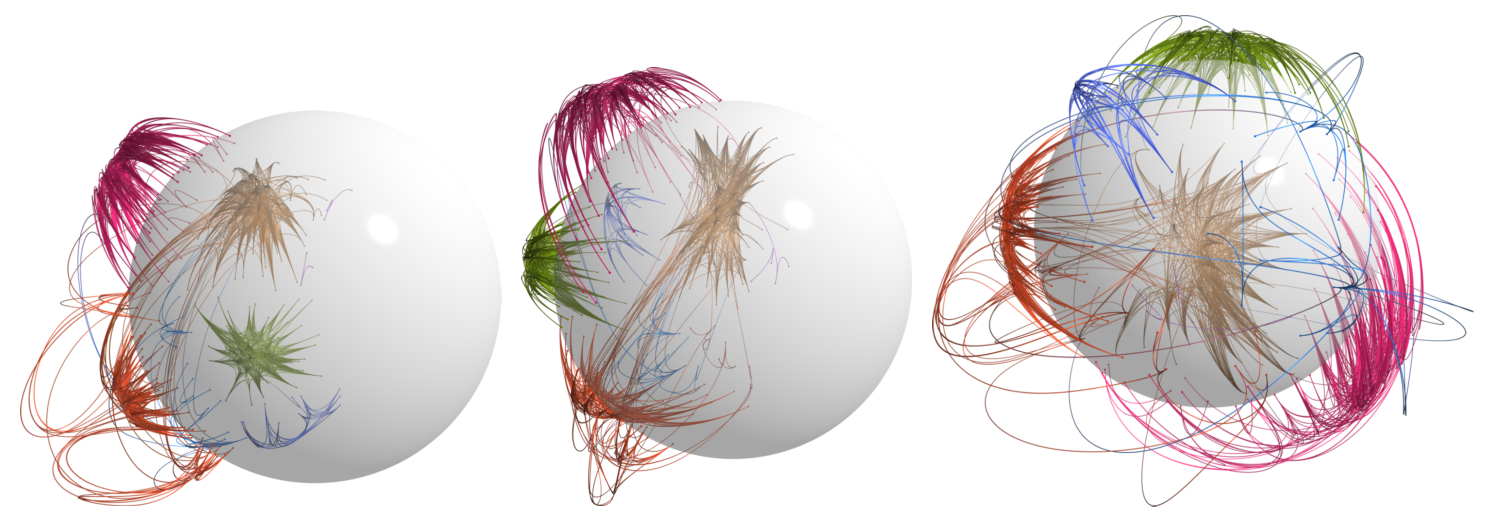
\includegraphics[width=14cm]{03_Figures/05_LitReview/Kwon2015_SphericalGraphLayout.png}
		\caption[2D layouts mapped to a sphere with varying amounts of distortion]{2D layouts mapped to a sphere with varying amounts of distortion:  \citep{Kwon2015}}
		\label{fig:sphericalgraph}
	\end{center}
\end{figure}


\subsubsection{Charts}

TODO: barchart, line-chart, pie-chart
TODO: advancement: rings with different speeds and colour?
\cite{CodeScience2015}

VR is a discipline that enables users to view large complex data sets in an intuitive and natural manner. For example it is possible to represent a particular data value as a 3D object (e.g. the size of a box can represent a parameter value within a dataset).
\cite{Jamieson2007}

Information visualization has relied on traditional methods, namely data mining techniques. [...] This data is usually visualized using 2D graphs, spread sheets, or quasi-3D structures but using a 2D medium (e.g. desktop monitor or projector). The ability to interact with the data is an advantage that data mining techniques does not easily fulfil, also there is a lack of feedback to the user, in timescales that could be considered useful. [...] Furthermore these methods do not scale well to the large multi-dimensional data sets. New methods are required that utilise the advantages of new technology (e.g. VR).
\cite{Jamieson2007}

In general, our visualization approach relies on multiple linked three-dimensional scatterplots which are presented and interacted with in a virtual environment, as shown in Figure 1. Each plot shows an arbitrary combination of three data attributes which are recorded per grid point. Time-dependent data is handled by animating the plots. All scatterplots are linked to each other, i.e., updates to a single plot become directly visible in all plots. This concept of linked views is combined with interactive brushing.
\cite{Hentschel2009}

\begin{figure}[h]
	\begin{center}
		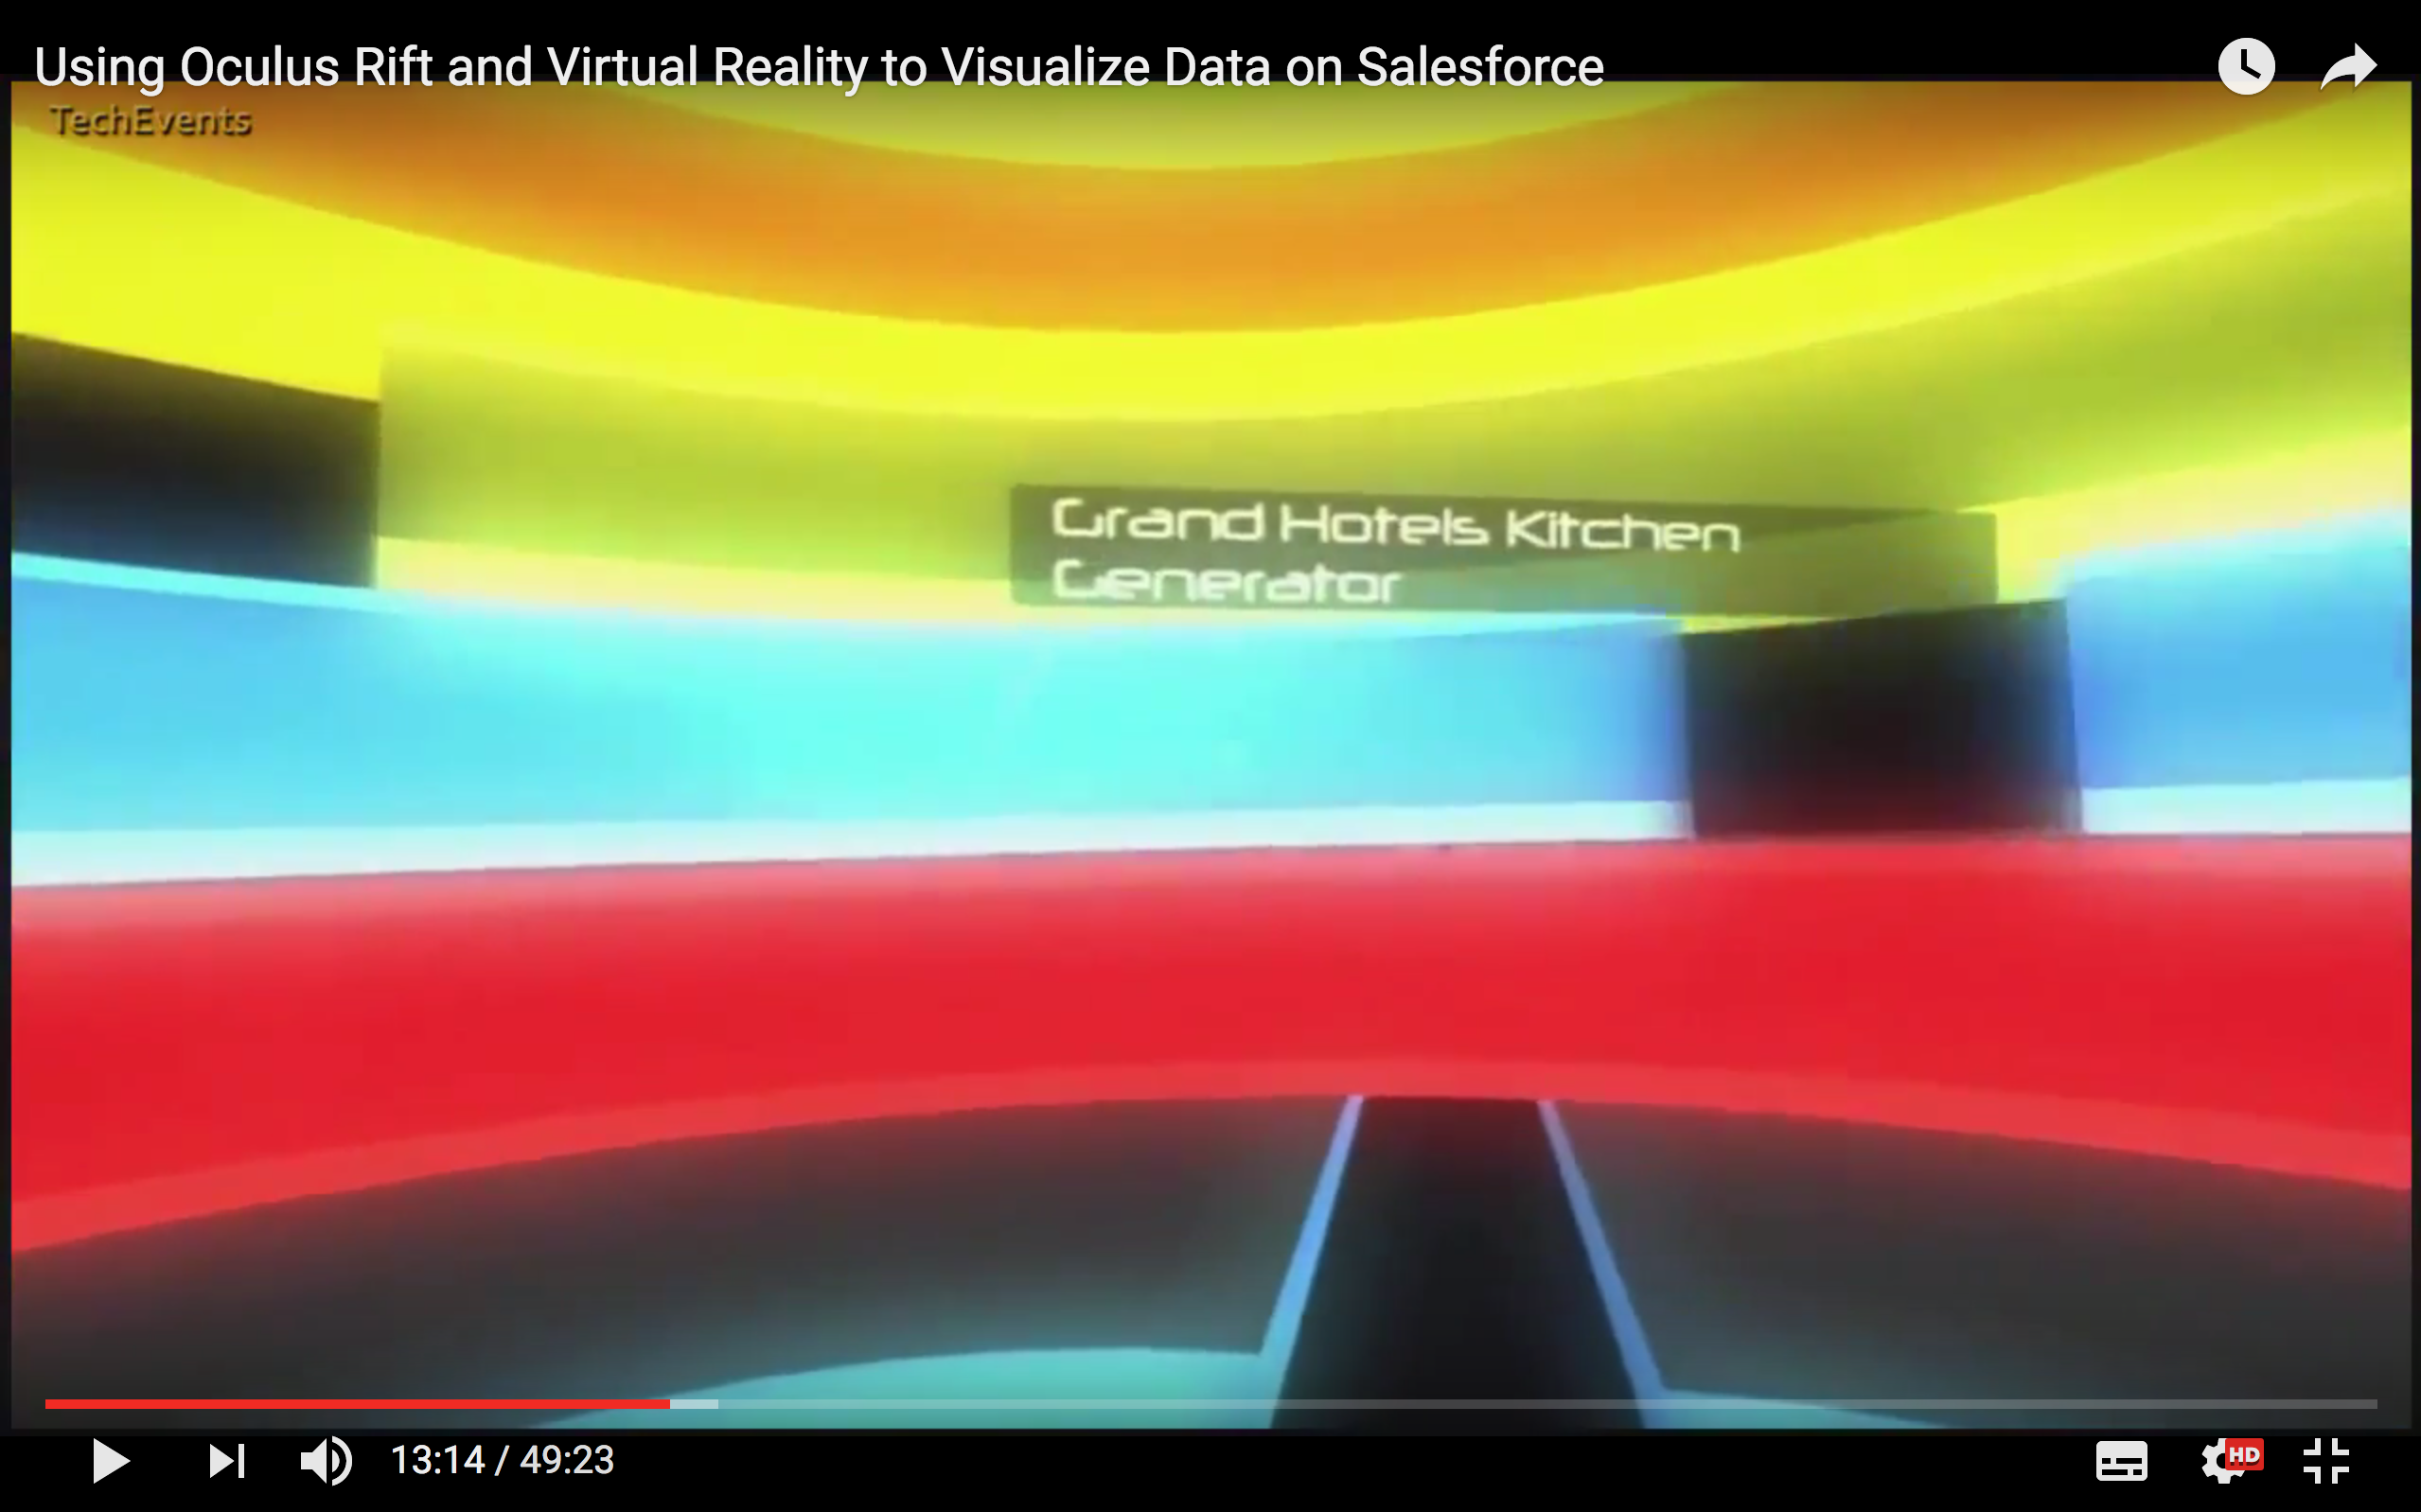
\includegraphics[width=14cm]{03_Figures/05_LitReview/CodeScience2015.png}
		\caption[Rotating data rings with varying speed in VR]{Rotating data rings with varying speed in VR \citep{CodeScience2015}}
		\label{fig:rotatingrings}
	\end{center}
\end{figure}


\begin{figure}[h]
	\begin{center}
		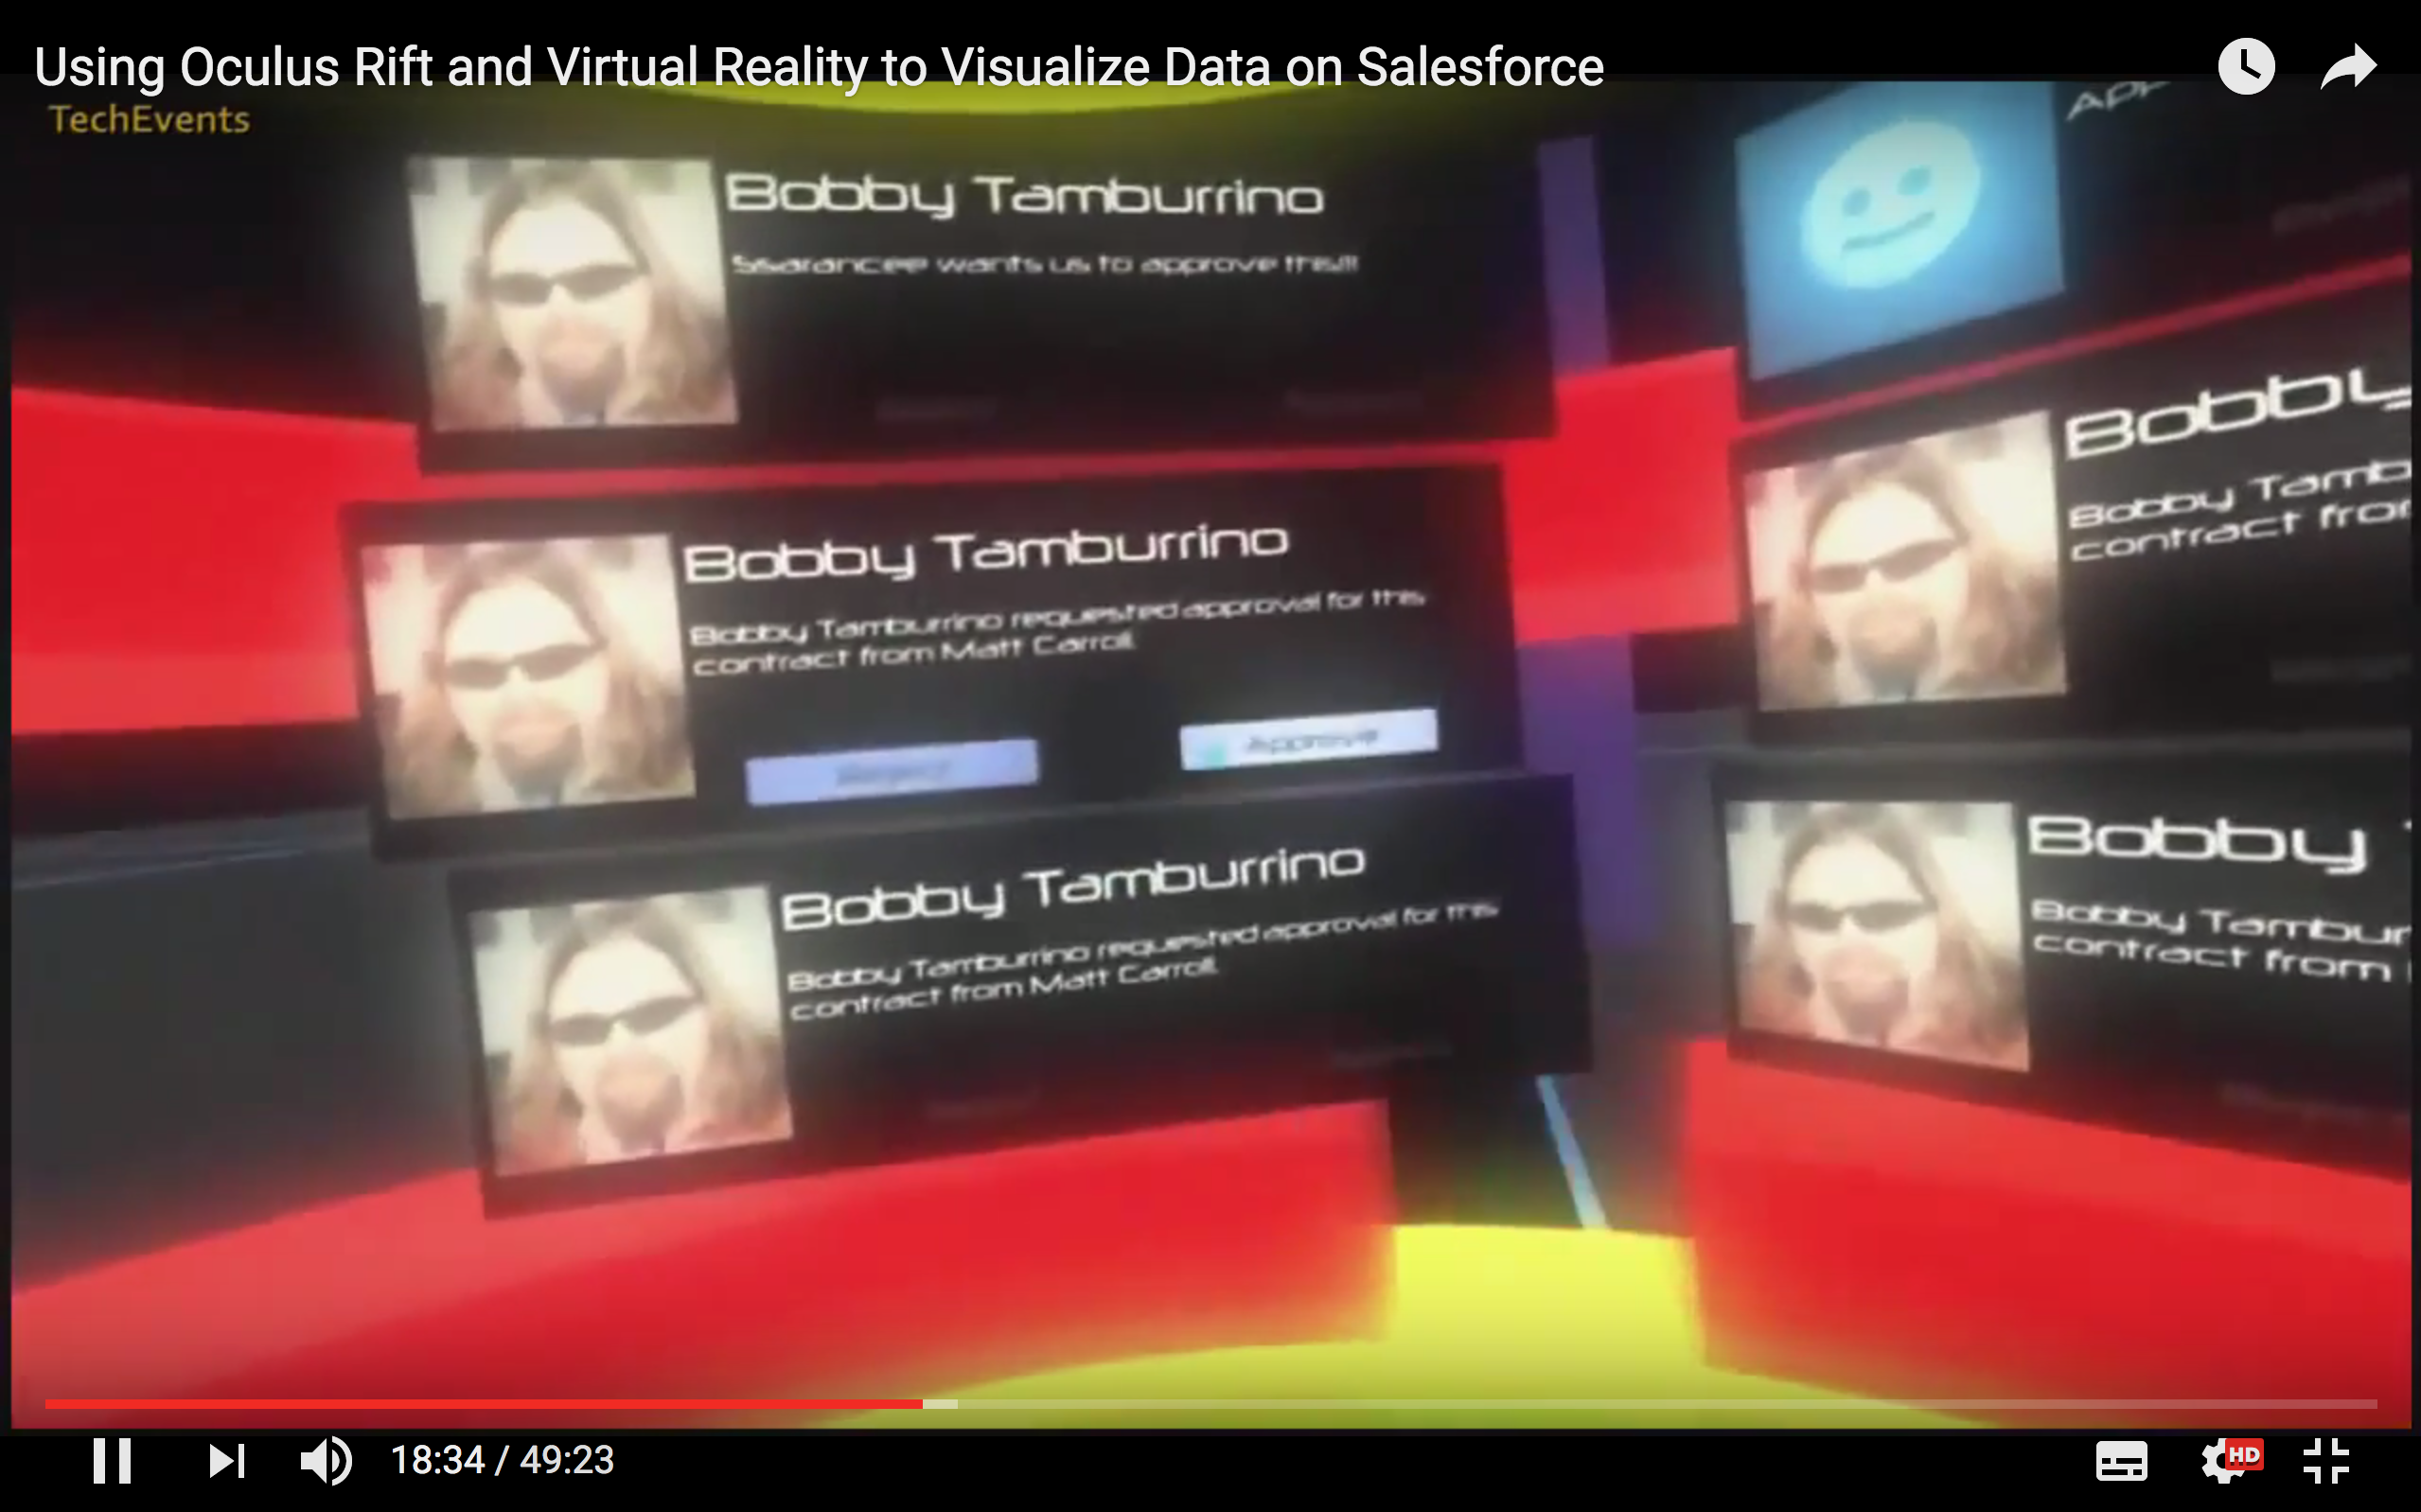
\includegraphics[width=14cm]{03_Figures/05_LitReview/CodeScience2015a.png}
		\caption[Detail view from a single rotating ring with multiple data displays]{Detail view from a single rotating ring with multiple data displays \citep{CodeScience2015}}
		\label{fig:rotatingringsdetail}
	\end{center}
\end{figure}


\begin{figure}[h]
	\begin{center}
		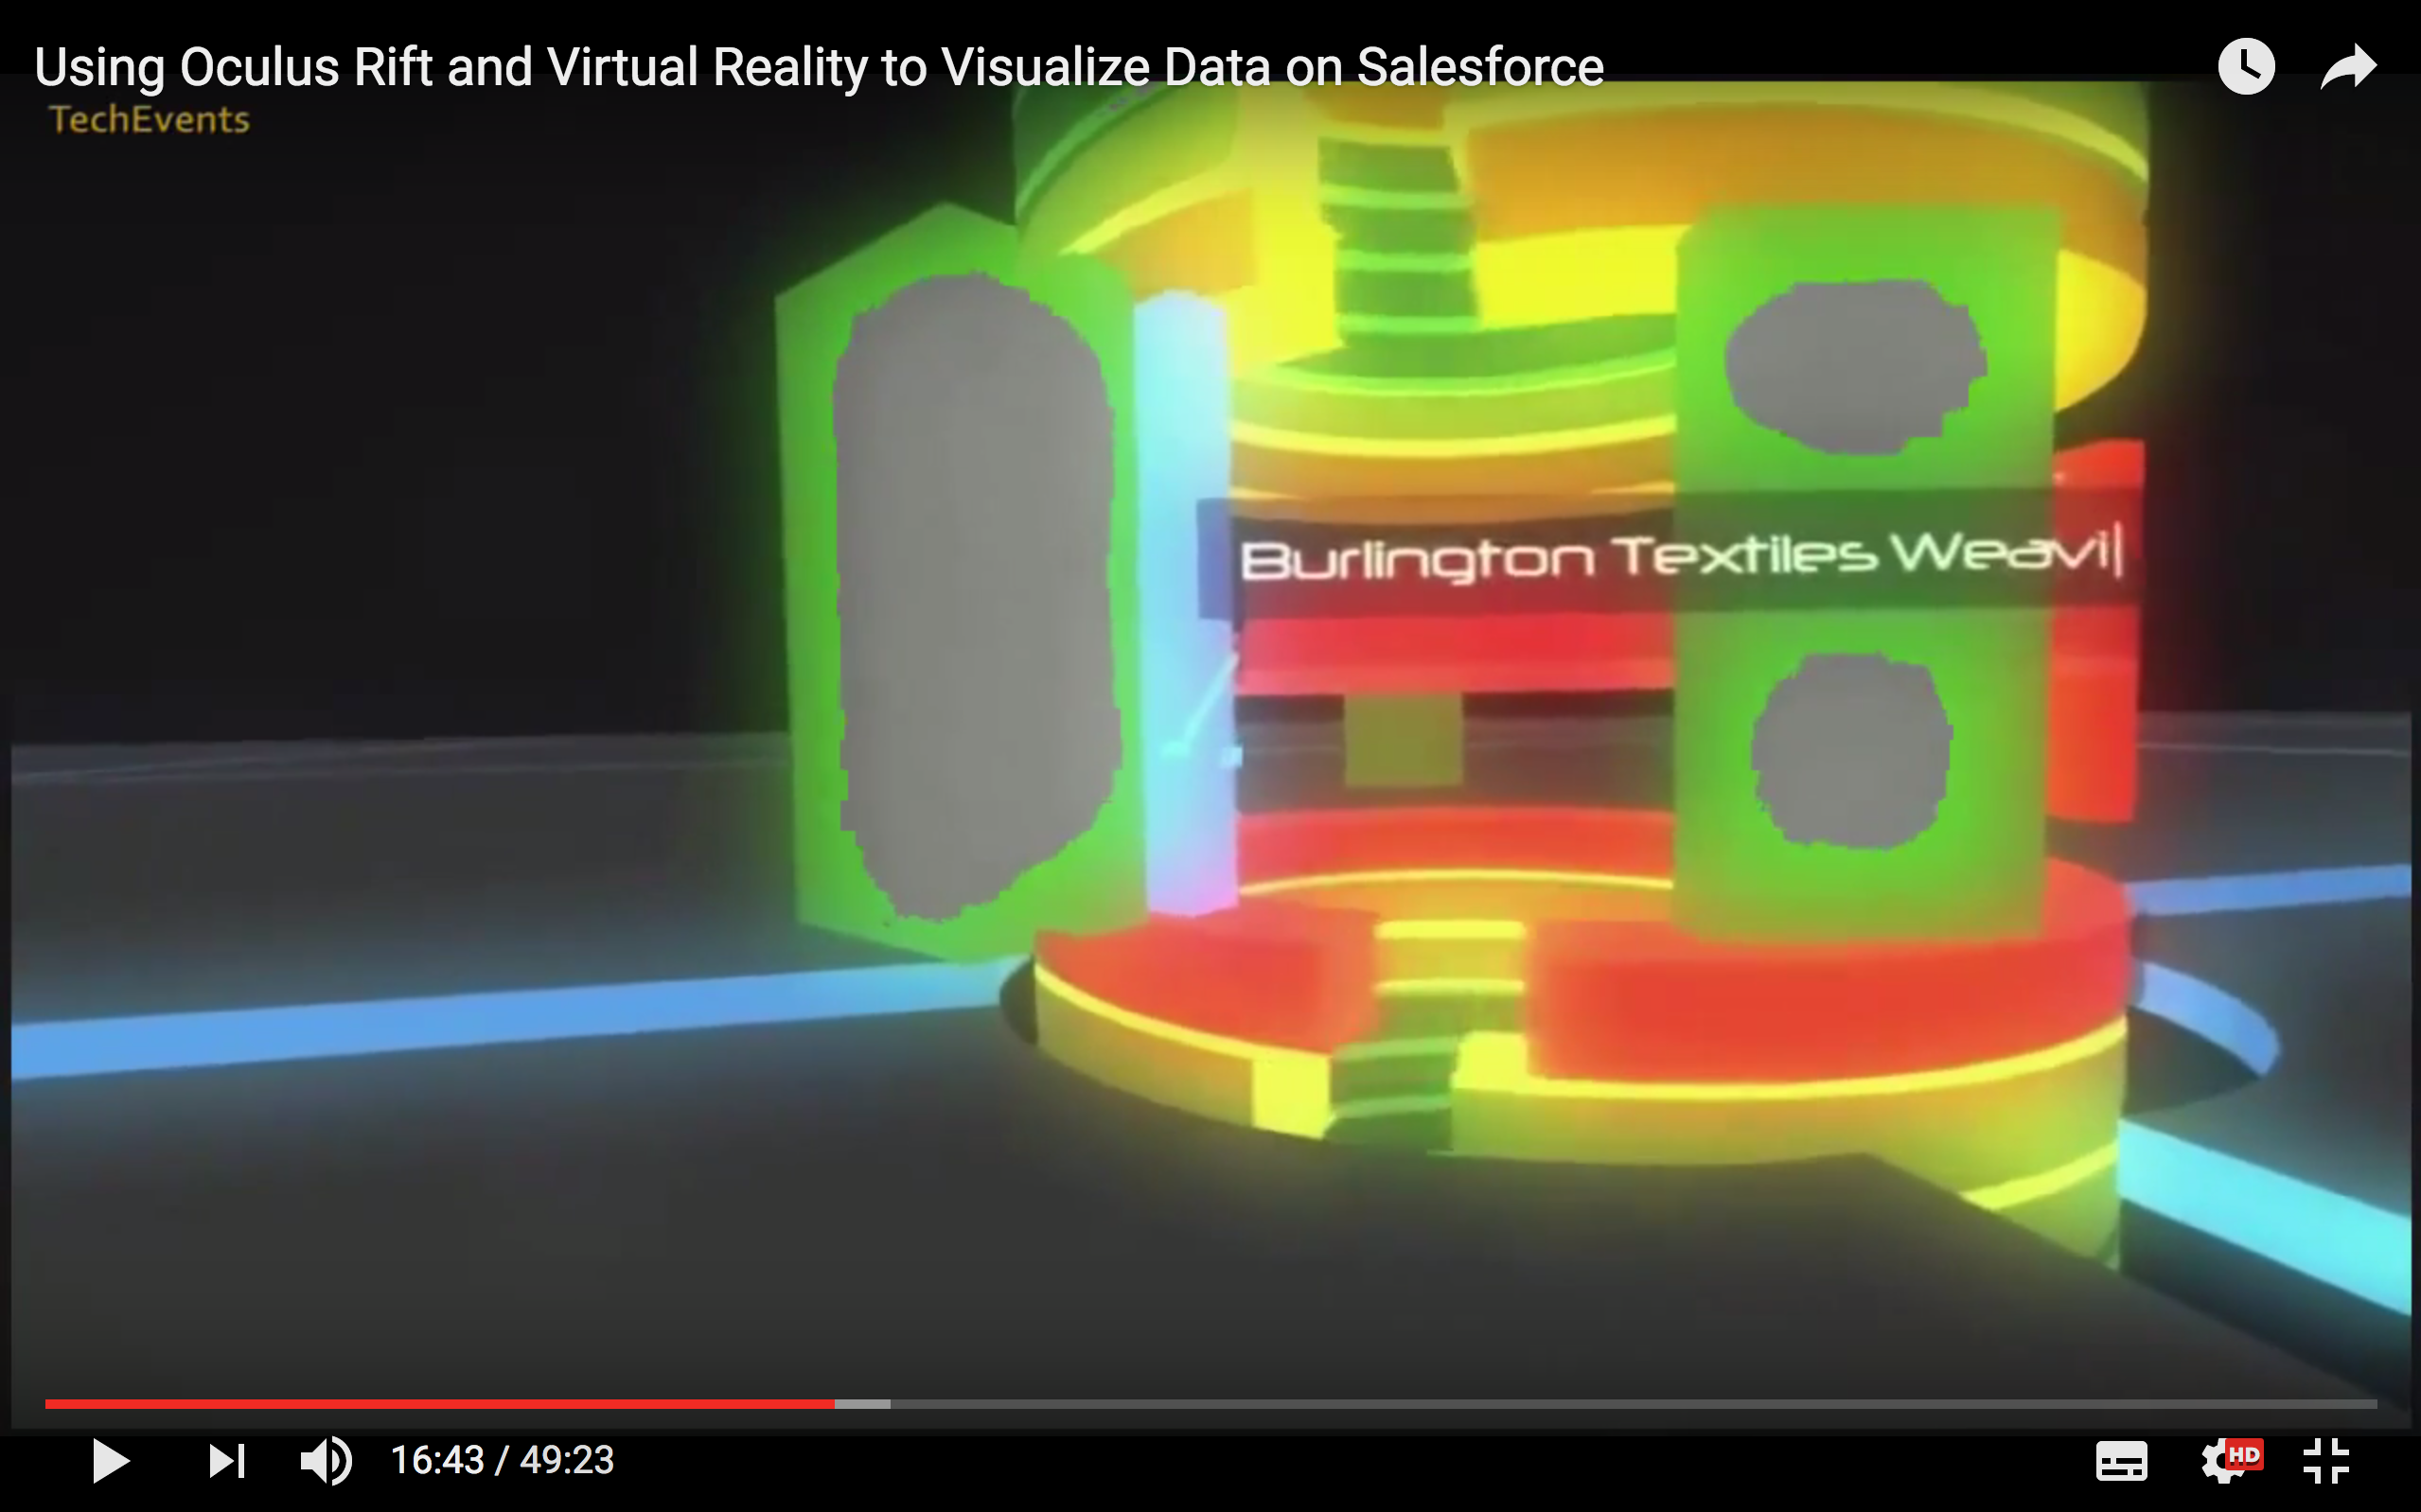
\includegraphics[width=14cm]{03_Figures/05_LitReview/CodeScience2015b.png}
		\caption[Outside view on tower built from rotating data rings with varying speed in VR]{Outside view on tower built from rotating data rings with varying speed in VR \citep{CodeScience2015}}
		\label{fig:rotatingringstower}
	\end{center}
\end{figure}


\subsubsection{Data-type-focused Presentation}

TODO: country maps with cantons (colour, shape, size), or grey-scale citymap with coloured houses (SimCity?)
TODO: advancement: unknown, no massive changes required?
TODO: Data-Forest!


Data with dimensionalities higher than three can be visualized by using multiple characteristics of the virtual objects. Examples include
Size (e.g. large, medium, small)
Shape (e.g. triangle, square, pentagon)
Color (e.g. red, purple, blue)
Texture (photographic images can be "painted" onto objects)
Position (X, Y, and Z)
Orientation (roll, pitch, yaw)
Behavior (spinning, bouncing, blinking, breathing, etc.)
Sound (chiming, singing, buzzing, etc.)
\cite{Stone1994}

Using our approach up to eight different parameters can be visualized by any one data tree. This number can be achieved by matching the physical properties of the tree (i.e. trunk and crown) to different parameters within the data set. The eight different parameters are listed below,
• position of the tree within the VE • height of trunk • width of trunk • colour of trunk • transparency value of the trunk • size of crown • colour of crown • transparency value of crown
\cite{Jamieson2007}

Stock Market Data: Therefore it is possible to match the movement of share prices with the changing shape/growth of the forest. An example of this can be seen in Figure 5.
\cite{Jamieson2007}

A dynamic forest will allow for the use of time variant information. A data tree has been chosen due to the fact that it is a simple object that people are familiar with. People can relate to making decisions on the size and shape of a tree relative to another.
\cite{Jamieson2007}

\begin{figure}[h]
	\begin{center}
		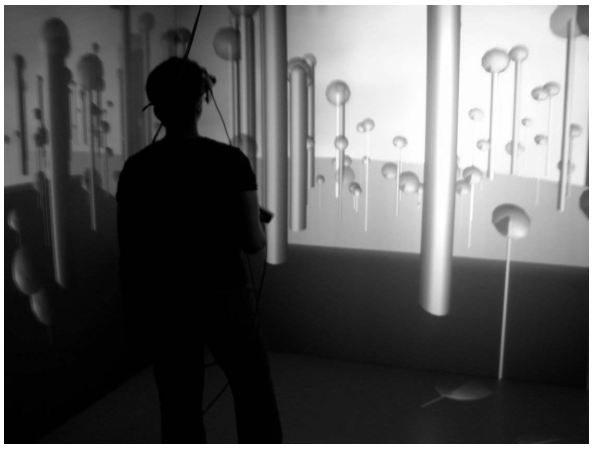
\includegraphics[width=7cm]{03_Figures/05_LitReview/Jamieson2007_DataTree.png}
		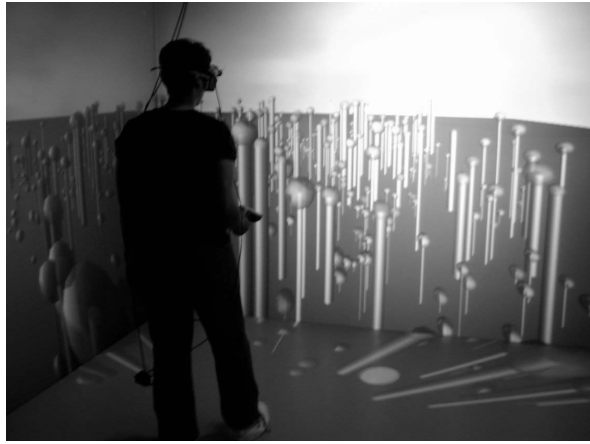
\includegraphics[width=7cm]{03_Figures/05_LitReview/Jamieson2007_DataTreeOverview.png}
		\caption[Navigation and Overview mode in a Data Forest]{Navigation (1) and Overview (2) mode in a Data Forest \citep{Jamieson2007}}
		\label{fig:datatrees}
	\end{center}
\end{figure} 

SphereViz interface: The 3D interface is designed for virtual reality (VR) environments. It presents a collection of image thumbnails in a virtual sphere as outlined in Figure 1. The position of a thumbnail in the sphere is determined by a number of parameters. These parameters either describe image properties such as total intensity, color proportions, etc, or characterize the image content.
\cite{Soldati2007}

\begin{figure}[h]
	\begin{center}
		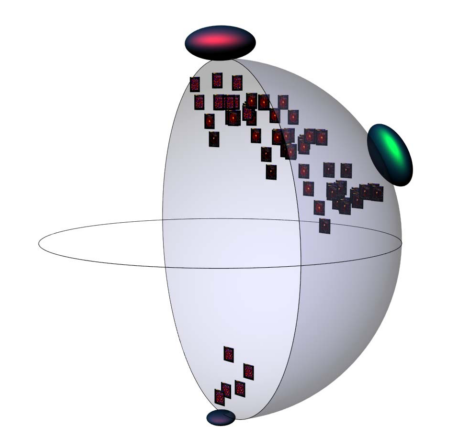
\includegraphics[width=7cm]{03_Figures/05_LitReview/Soldati2007_SphereViz.png}
		\caption[Schematic view of SphereViz where parameters influence the position of data objects]{Schematic view of SphereViz where parameters (ellipsoids) influence the position of data objects (rectangles) \citep{Soldati2007}}
		\label{fig:sphereviz}
	\end{center}
\end{figure} 

SphereViz benefits from the advanced spatial visualisation and interaction methods provided by Virtual Reality. Spatial visualisation allows presenting clusters of images in a very user friendly way, spatial interaction is used for evaluation and searching tasks. VR increases the legibility of large datasets and provides more intuitive techniques for browsing through the data.
\cite{Soldati2007}

Visualized data objects are characterized by three attributes: size, scale, and distance. They play an important role for a better understanding of the displayed data in particular because the objects are perceived in "natural scale".
\cite{Soldati2007}

%-----------------------------------
%	SUBSECTION 3
%-----------------------------------

\subsection{Data Manipulation}

TODO: Data manipulation
TODO: Rename to something like "Work with data"?

"Direct Manipulation of Graphical Objects" since 1960 in University Research, since 1970 in Corporate Research and since 1980 in Commercial Products.
\cite{Myers1998}

A visualization goal is to simplify the analysis of large-quantity, numerical data by rendering the data as an image that can be intuitively manipulated.
\cite{Stone1994}

I see VRs as having three important characteristics: First, VRs exhibit high interactivity - there is a tight coupling between the user's actions and the feedback generated by those actions. Second, they support embodiment: some sort of representation of the user is in the same spatial framework as the data. Third, the VR representation is spatial in nature; virtual objects are situated in a spatial framework
\cite{Stone1994}

Second, visualization is entwined with manipulation. We don't just want to look at data, we want to move around it, twist it, shake it, change its color mapping, expand it, rotate it, shrink it, or slice and dice it.
\cite{Stone1994}

VR allows us to create Virtual Environments (VEs) in which we can render our 3D objects representing our data. The advantage that these VEs have over traditional approaches is that they allows us to be immersed within the data. We can use methods to examine the different features of the data that are more intuitive to us. An example of this is the ability to track the users head position so that we can appear to look around object, this is how as humans we are familiar with examining objects of interest, rather than moving a mouse. In a totally immersive virtual environment we can use body movement to walk around objects or put our head inside virtual representation of our data. Also within an immersive environment it is possible to map the users hand position in the real world to a virtual hand in the VE, therefore allowing the user to manipulate virtual objects.
\cite{Jamieson2007}

“Drilling down” is a common term in mentioned in data mining techniques, but here we have taken the approach of “exposing the roots” of the data tree. Users can choose a particular tree that they are interested in by using their input device to “touch” the tree, then using a 3D menu (see Figure 3) choose to further examine the related data.
\cite{Jamieson2007}

From an interaction point of view, the user can now walk through the virtual world and inspect groups of
thumbnails or magnify single thumbnails. Additionally he or she can grab the parameter handles and move them freely on the sphere surface. This will cause the thumbnails to be re-arranged in real-time. This visible movement gives valuable feedback to the user.
\cite{Soldati2007}

Users can freely walk in the virtual world and interact with virtual data objects. They can control the visualization by natural actions like grabbing or moving objects. Thumbnails that are covered by an other object can be brought
to the foreground just by walking around the object. Thus, the user can focus on his or her main task, without bothering about input devices.
\cite{Soldati2007}

The World in Miniature (WIM) is an interface technique that uses a virtual hand-held miniature copy of the immersive virtual scene for visualization and interaction tasks. In addition to the first-person perspective offered by a virtual environment, WIM offers a second dynamic perspective onto the scene. Objects can be manipulated directly in the immersive scene or through the WIM.
\cite{Soldati2007}

We see a great potential in using VR for visual exploration of multi-dimensional data sets and in particular in SphereViz. Amongst others driven by the game industry, we expect VR technology to evolve significantly within the next 10 to 15 years. VR will allow users to look at and interact with large datasets in new ways.
\cite{Soldati2007}

Taking the Visual Information-Seeking Mantra into account [9] the current application covers the zoom and filter and the details on demand part. In future versions we plan to extend the WIM to give the overview of all available data.
\cite{Soldati2007}

The analysis of time-dependent simulation data is a demanding task, both in terms of computing power and time. Interactive analysis using multiple linked views has been shown to be one possible solution to this problem. However, there are two significant short- comings when limited to a standard desktop-based setup: First, complex spatial relationships are hard to understand using only 2D projections of the data. [...]
\cite{Hentschel2009}

Traditionally, researchers look at 3D volume renderings on desktop computer monitors or larger displays, which lack the more realistic visual stimuli found in more advanced displays, such as stereoscopic 3D graphics and motion parallax due to head tracking. Thus, it may be more difficult for the user to judge the size, shape, or depth of the structures in the volume data. Judgments of this sort are required not only for general understanding, but also for performing interactive tasks such as segmentation of a dataset. Conducting such tasks with traditional displays, therefore, may result in slower performance and/or erroneous interpretation.
\cite{Laha2012}

We conducted a controlled empirical study in which we studied the independent and combined effects of three components of immersion (head tracking, FOR, and stereoscopic rendering) on the analysis of two different volume-visualized microscopic computed tomography (micro-CT) datasets. We found significant positive effects of these components of immersion, but the results also show that the effects are dependent on how the components are combined and on the type of analysis task.
\cite{Laha2012}

We found that most of the benefits of high immersion for analyzing volume data are positive. Of the three components of immersion that we evaluated in our controlled study, FOR had the most positive effects on the widest range of tasks. However, levels of immersion have differential effects on different tasks. We observed the most positive effects of immersion for tasks involving visually and spatially complex search for features in the volume datasets. General descriptive tasks showed mixed effects of immersion. Users showed mixed preferences for the different levels of immersion. They felt that stereoscopic vision made it easier to understand features of a volume dataset, and head-based rendering provided greater ease of obtaining the desired view they wanted and of exploring the datasets in general.
\cite{Laha2012}

VR has been shown to lead to better discovery in domains that whose primary dimensions are spatial.
\cite{Donalek2014}

\begin{figure}[h]
	\begin{center}
		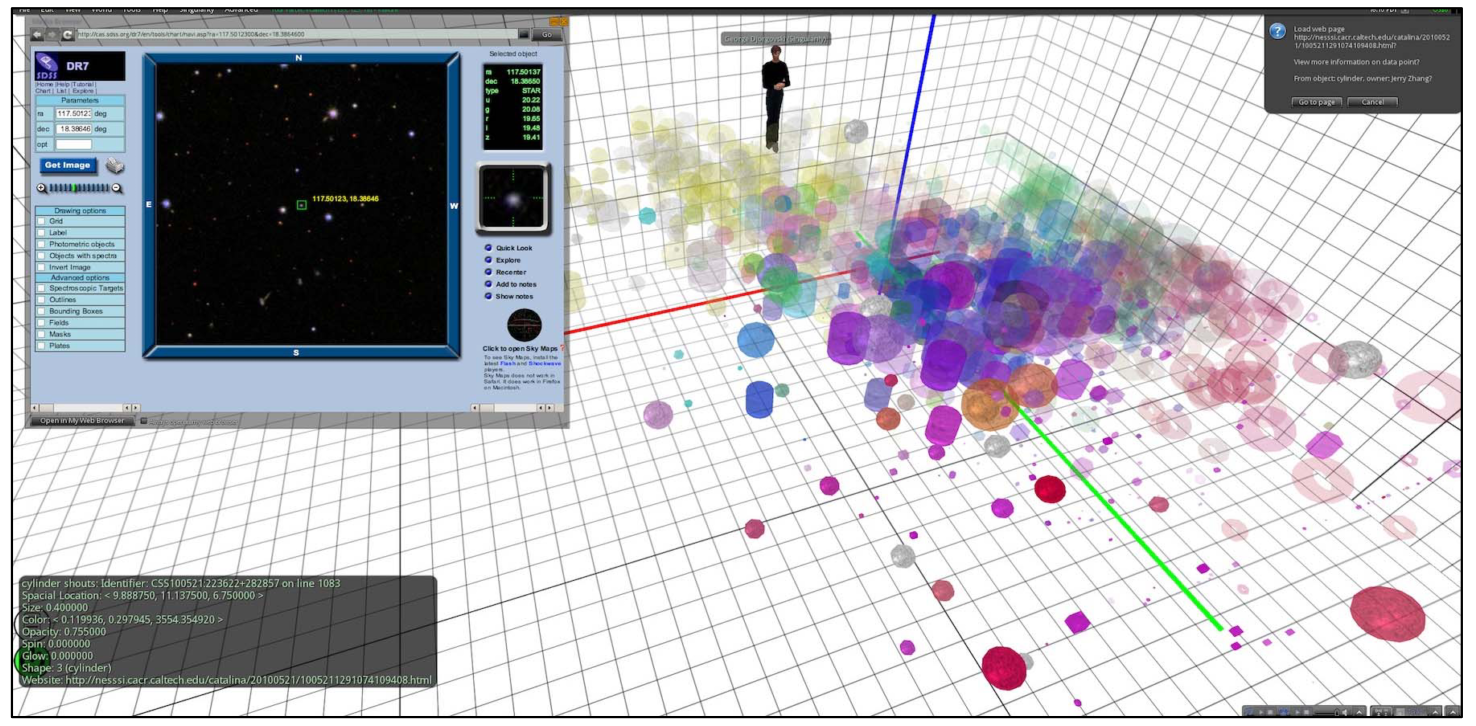
\includegraphics[width=14cm]{03_Figures/05_LitReview/Donalek2014_Caltech.png}
		\caption[Data visualization experiments in the OpenSim-based virtual world vCaltech]{Data visualization experiments in the OpenSim-based virtual world vCaltech \citep{Donalek2014}}
		\label{fig:caltechsim}
	\end{center}
\end{figure}

\begin{figure}[h]
	\begin{center}
		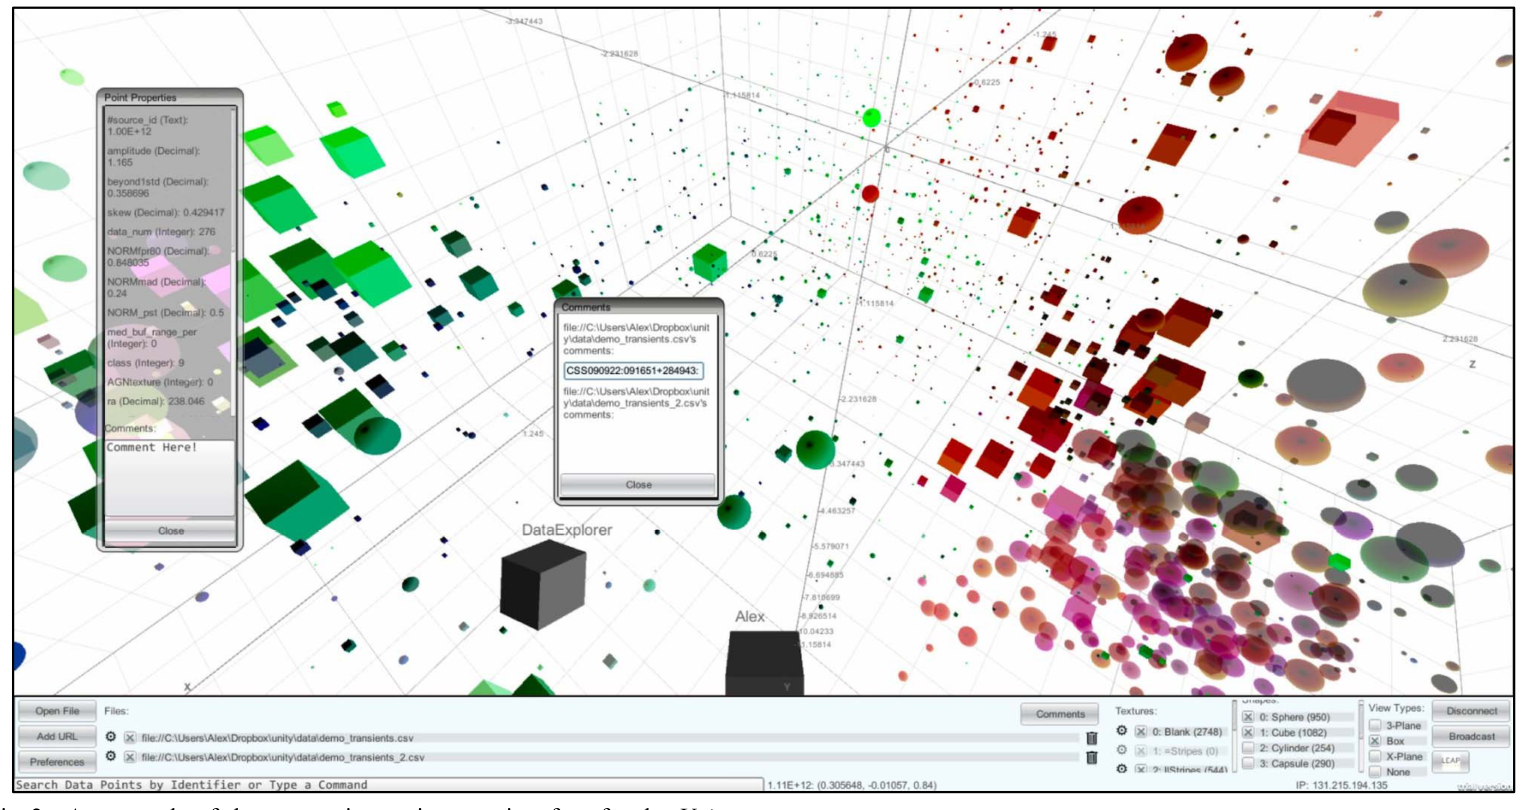
\includegraphics[width=14cm]{03_Figures/05_LitReview/Donalek2014_iViz.png}
		\caption[Example of an interactive user interface for the Unity-based data visualizer, iViz]{Example of an interactive user interface for the Unity-based data visualizer, iViz \citep{Donalek2014}}
		\label{fig:iviz}
	\end{center}
\end{figure}


In this project, our objective is to lower the barriers to entry for exploratory analysis of complex scientific data by leveraging the Oculus Rift to provide intuitive interactions and efficient navigation in an immersive 3D environment
\cite{Drouhard2015}

There are clear advantages to conventional two-dimensional (2D) techniques, such as the bar chart and the scatterplot. The most powerful pattern-finding mechanisms of the brain work in 2D, not 3D. Designers already know how to draw diagrams and represent data effectively in two dimensions, and the results can easily be included in books and reports. Of course, one compelling reason for an interest in 3D space perception is the explosive advance in 3D computer graphics.
\cite{Ware2012}

We still lack design rules for 3D environments, and many interaction techniques are competing for adoption. The strongest argument for the ultimate ascendancy of 3D visualization systems, and 3D user interfaces in general, must be that we live in a 3D world and our brains have evolved to recognize and interact within 3D. The 3D design space is richer than the 2D design space, because a 2D space is a part of 3D space. It is always possible to flatten out part of a 3D display and represent it in 2D.
\cite{Ware2012}

Nevertheless, it also should be cautioned that going from 2D to 3D adds far less visual information than might be supposed. Consider the following simple argument. On a one-dimensional line of a computer display, we can perceive 1000 distinct pixels. On a 2D plane of the same display, we can display 1000 × 1000 = 1,000,000 pixels, but going to a 3D stereoscopic display only increases the number of pixels by a factor of 2, and this does not double the available information because the two images must be highly correlated for us to perceive stereoscopic depth.
\cite{Ware2012}

They examine how traditional methods for 2D User interface/User Experience usability evaluation may be applied to VR interfaces. They also discuss subjective measures that should be used to assess VR applications, including user comfort and ease of use. --> 12 (Bowman2012a)
\cite{Drouhard2015}

In the case of scientific analysis, the transition to a 3D environment can be difficult, as most scientists typically explore their data using 2D visualizations, and they have been doing so for decades. Careful thought should be devoted to ways to capture the essence of the most effective 2D interactions and bring them to bear in a 3D display.
\cite{Drouhard2015}


brainstorming
- click to select/highlight/focus   --> click with controller
- click+drag to re-order / rotate	--> re-order remains the same, rotate by walking (!!)
- click+drag to select area to zoom   --> walking closer, maybe select range with controllers
- mouse-wheel to zoom in/out   --> zoom by walking closer (!!)
- right-lick for context menu (add, remove, ...)   --> click with controller
- enable/disable with checkboxes

currently primarily done with mouse which can be 1:1 substituted with a gesture controller
BUT use 3d space to utilize walking option


%-----------------------------------
%	SUBSECTION 4
%-----------------------------------

\subsection{Conclusion}

TODO: summarize srq3 chapter

%This literature review has shown that...
% to be completed (\gls{vism} 3.0 ?)



%----------------------------------------------------------------------------------------
%	SECTION 4
%----------------------------------------------------------------------------------------

\section{Conclusion}

\label{SectionLiteratureReviewConclusion}

TODO: summarize the whole chapter 2



\fillingPage{}
%----------------------------------------------------------------------------------------
%	CHAPTER - RESEARCH METHOD
%----------------------------------------------------------------------------------------

\chapter{Research Method} % Main chapter title

\label{Research Method} % Change X to a consecutive number; for referencing this chapter elsewhere, use \ref{ChapterX}

%----------------------------------------------------------------------------------------
%	SECTION 1
%----------------------------------------------------------------------------------------

\section{Introduction}

In this chapter, the research methodology of this thesis is described. An interpretive research philosophy is assumed for this thesis. \cite{Hevner2010} defined different research strategies out of which design science is applied.


%----------------------------------------------------------------------------------------
%	SECTION 2
%----------------------------------------------------------------------------------------

\section{Philosophy}

The research philosophy shows how the researcher views the world and the knowledge that has to be developed as well as its nature.

\cite{Saunders2009} defines four different research philosophies:
\begin{itemize}[noitemsep,nolistsep]
	\item Positivism \textit{(only observable phenomena will lead
		to the production of credible data)}
	\item Realism \textit{(do objects exist independently of our
		knowledge of their existence?)}
	\item Interpretivism \textit{(understanding differences 
		between humans as social actors)}
	\item Pragmatism \textit{(do you have to adopt one position?)}
\end{itemize}

In addition, \cite{Saunders2009} also lists three major ways of how to think about the different research philosophies:
\begin{itemize}[noitemsep,nolistsep]
	\item Epistemology \textit{(the view of the nature of reality or being)}
	\item Ontology \textit{(the view of what constitutes acceptable knowledge)}
	\item Axiology \textit{(the view of the role of values in research)}
\end{itemize}

% TODO: check for Vaishnavi reference
An interpretive research philosophy, as defined by \cite{Vaishnavi2008} and \cite{Saunders2009}, is assumed for this thesis since it has the biggest match out of all possible philosophies. The reason for this can be found upon evaluating the different views. \newline
Gesture controllers and 360° motion tracking provide, from a technical point of view, a standard input device. What individuals actors do with the available means however is completely subjective. From an \textbf{epistemology view}, the researcher interprets the presented situation and his actions are motivated based on how he percepts the details of this situation. \newline
In the \textbf{ontology view}, the researcher's view of the nature of reality is socially constructed, subjective and may change. In virtual reality, everything depends on how he perceives and interprets the visualizations; every individual has a different view of the reality. \newline
From the \textbf{axiology view}, the view of what role the values play, the researcher is part of what is being researched as he decides on his own how to interact with the virtual reality and what usable gestures are defined. This is subjective as it cannot be separated from the research and thus there will be not the one solution, but merely one out of many. \newline
Finally, looking at the data collection methods, only small samples of sensor data from gesture controllers and 360° motion tracking will be collected. This data can be investigated quantitative (is the gesture effective in its purpose?), qualitative (does the gesture what I intended to do?) or also in combination


%----------------------------------------------------------------------------------------
%	SECTION 3
%----------------------------------------------------------------------------------------

\section{Approach}

Based on \cite{Saunders2009}, a research approach can either be deductive (testing a theory), inductive (building a theory) or a combination of them. Table \ref{tbl:inductivedeductive} shows the major differences between deductive and inductive approach.
\begin{table}[h!]
	\begin{center}
		\begin{tabular}{ p{6.5cm} p{7.5cm} }
			\toprule
			\textbf{Deduction emphasises} & \textbf{Induction emphasises} \\
			\midrule
			scientific principles & less concern with the need to generalise \\
			moving from theory to data & a close understanding of the research context  \\
			the need to explain causal relationships between variables & gaining an understanding of the meanings humans attach to events \\
			the collection of quantitative data & the collection of qualitative data \\
			the application of controls to ensure validity of data & a more flexible structure to permit changes of research emphasis as the research progresses \\
			the operationalisation of concepts to ensure clarity of definition & a realisation that the researcher is part of the research process \\
			a highly structured approach & \\
			researcher independence of what is being researched & \\
			the necessity to select samples of sufficient size in order to generalise conclusions & \\
			\bottomrule
		\end{tabular}
		\caption[Major differences between deductive and inductive approaches to research]{Major differences between deductive and inductive approaches to research (adopted from {\citealp[pg. 127]{Saunders2009}})}
		\label{tbl:inductivedeductive}
	\end{center}
\end{table}
\newline
With literature review, knowledge about the current state of interaction possibilities with virtual reality is collected and analysed. Based on the gained information and a close understanding of the research context, a theory can be formulated. With the help of a to be built prototype this theory can be evaluated and tested by the researcher. This is a typical procedure of an inductive approach as described by \cite{Saunders2009}. \newline
The deductive approach starts at the other end as first the theory is built by searching to explain causal relationships between variables. The test of this theory requires the collection of quantitative data which does not match the goal of this thesis, since its focus is more theoretical. \newline
\cite{Creswell2014} further defined a set of criteria for selecting a research approach based on the situation of current research. If only little research has been done yet and the topic first has to be explored and understood, then a qualitative (inductive) approach suits the best \citep[pg 50]{Creswell2014}. Although virtual reality in itself has been researched for quite a while, it indeed is quite new to have gesture controllers and 360° motion tracking available as well. This makes the thesis a good match for an inductive approach.


%----------------------------------------------------------------------------------------
%	SECTION 4
%----------------------------------------------------------------------------------------

\section{Strategy}

%-----------------------------------
%	SUBSECTION 1
%-----------------------------------

\subsection{Introduction}

\cite{Saunders2009} consider seven different research strategies:
\begin{itemize}[noitemsep,nolistsep]
	\item Experiment \textit{(study causal links)}
	\item Survey \textit{(answering who, what, where, how much and how many questions)}
	\item Case Study \textit{(empirical investigation within its real life context)}
	\item Action Research \textit{(explicit focus on research in action)}
	\item Grounded Theory \textit{(emphasis upon developing and building a theory)}
	\item Ethnography \textit{(describe and explain the social world the research subjects inhabit)}
	\item Archival Research \textit{(administrative records and documents as principle data source)}
\end{itemize}
In Information Systems, \cite{Hevner2010} suggest \textbf{design science} as another research strategy which inherently is a problem solving process. For this strategy, seven guidelines for design science research are derived which can be summarized in two main characteristics \citep{Hevner2010}: On the one hand the creation of an innovative, purposeful artefact for a specified problem domain, and on the other hand the thorough evaluation of the artefact and its highly applicable in practice. Both of them are considered crucial for this thesis. \newline
The artefact is represented by the prototype of a virtual reality application that utilizes the additional sensor information from gesture controllers and 360° motion tracking. The relevance for practice and its applicability is given by feasible enhancements to existing solutions that are already used in practice.



%-----------------------------------
%	SUBSECTION 2
%-----------------------------------

\subsection{Design Research Cycle}

\cite{Vaishnavi2008} and \cite{Hevner2010} define \gls{dsr} as a research paradigm in which questions that are relevant to human problems are answered with the creation of innovative artefacts. As an approach for conducting design science research, \cite{Vaishnavi2004} defined a design science research process model (\gls{dsr} Cycle). This cycle follows a step-wise approach and has been structured in the five phases that are as follows: awareness of the problem, suggestion, development, evaluation and conclusion (Figure \ref{fig:dsrcycle}). In the following chapters, these five phases and their relation to this thesis are discussed.
\newline
%    h (here) - same location
%    t (top) - top of page
%    b (bottom) - bottom of page
%    p (page) - on an extra page
%    ! (override) - will force the specified location
\begin{figure}[h]
	\begin{center}
		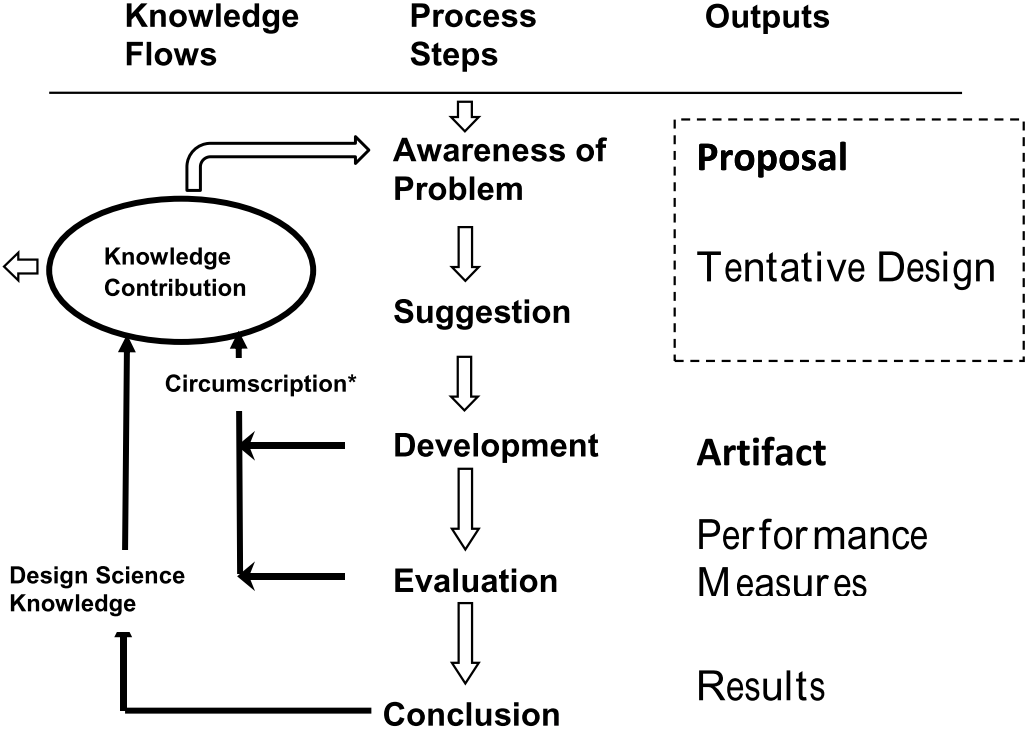
\includegraphics[width=11cm]{03_Figures/02_DSR_Cycle/DSR_Cycle.png}
		\caption[Design Science Research Process Model (DSR Cycle)]{Design Science Research Process Model (DSR Cycle) \citep{Vaishnavi2004}}
		\label{fig:dsrcycle}
	\end{center}
\end{figure}


%-----------------------------------
%	SUBSUBSECTION 1
%-----------------------------------

\subsubsection{Awareness}

\cite{Hevner2010} defined in the initial step of the \gls{dsr} Cycle the awareness of the problem, where
\begin{itemize}[noitemsep,nolistsep]
	\item the problem is identified.
	\item the problem is defined.
	\item the value of a solution is justified.
\end{itemize}
This is the foundation of all subsequent steps as the suggestion, development and evaluation phases all focus on the identified problem. \newline
In this thesis, the identification and definition of the problem is covered in chapter \ref{ChapterIntroduction} (introduction) whereas the justification of the value of a solution is established in the literature of chapter \ref{ChapterLiteratureReview} in the form of research gaps.
The literature review shows that while there has been research done on the interaction patterns for \textit{Travel} and \textit{Selection}, the \textit{Motivation} is only covered on the surface. Furthermore, although guidelines for the interaction patterns are available, there are no practical suggestions/recommendations on how this could look like in practice or whether these guidelines really make sense once applied. The motivation for an improvement lies in the importance of \textit{Manipulation} patterns or uses in practice and recommendations on how matching interactions patterns have to be designed with the corresponding method in mind.


%-----------------------------------
%	SUBSUBSECTION 2
%-----------------------------------

\subsubsection{Suggestion}

blub


%-----------------------------------
%	SUBSUBSECTION 3
%-----------------------------------

\subsubsection{Development}

In the development phase, the existing knowledge together with the defined problem definition is synthesized into an artefact that solves the mentioned problem \citep{Vaishnavi2008}. In this thesis, the artefact is the virtual reality prototype application.


%-----------------------------------
%	SUBSUBSECTION 4
%-----------------------------------

\subsubsection{Evaluation}

In order to demonstrate that with the proposed solution the problem can be solved, \cite{Hevner2010}  defined that the artefacts needs to be evaluated.
Table XXX shows possible evaluation methods for designed artefacts  that are based on \cite{Hevner2004}. For this research, the methods from \textit{Testing} and \textit{Descriptive} will be applied.


\begin{table}[h]
	\begin{center}
		\begin{tabular}{ | m{4cm} | p{10cm} | } 
			\hline
			\multirow{2}{*}{1. Observational} &
				Case Study: Study artefact in depth in business environment \\
				\cline{2-2}
				& Field Study: Monitor use of artefact in multiple projects \\
			\hline
			\multirow{4}{*}{2. Analytical} &
				Static Analysis: Examine structure of artefact for static qualities (e.g., complexity) \\
				\cline{2-2}
				& Architecture Analysis: Study fit of artefact into technical IS architecture \\
				\cline{2-2}
				& Optimization: Demonstrate inherent optimal properties of artefact or provide optimality bounds on artefact behaviour \\
				\cline{2-2}
				& Dynamic Analysis: Study artefact in use for dynamic qualities (e.g., performance) \\
			\hline
			\multirow{2}{*}{3. Experimental} &
				Controlled Experiment: Study artefact in controlled environment for qualities (e.g., usability) \\
				\cline{2-2}
				& Simulation - Execute artefact with artificial data \\
			\hline
			\multirow{2}{*}{4. Testing} &
				Functional (Black Box) Testing:  Execute artefact interfaces to discover failures and identify defects \\
				\cline{2-2}
				& Structural (White Box) Testing:  Perform coverage testing of some metric (e.g., execution paths) in the artefact implementation \\
			\hline
			\multirow{2}{*}{5. Descriptive} &
				Informed Argument:  Use information from the knowledge base (e.g. relevant research) to build a convincing argument for the artefact's utility \\
				\cline{2-2}
				\cline{2-2}
				& \cellcolor{green!25}Scenarios: Construct detailed scenarios around the artefact to demonstrate its utility \\
			\hline
		\end{tabular}
		\caption[here]{bbilbio}
		\label{tbl:designevaluationmethods}
	\end{center}
\end{table}


%-----------------------------------
%	SUBSUBSECTION 5
%-----------------------------------

\subsubsection{Conclusion}

blub


%----------------------------------------------------------------------------------------
%	SECTION 5
%----------------------------------------------------------------------------------------

\section{Timeline}

As part of the master thesis research proposal, the literature review is conducted alongside its analysis. The development and evaluation of the prototype as part of the design science research will be done in the implementation phase of the master thesis.


%----------------------------------------------------------------------------------------
%	SECTION 6
%----------------------------------------------------------------------------------------

\section{Data collection}

Quantitative vs Qualitative

--> check The research choice defines how data is collected or analysed. This can be either in a quantitative way (numerical data) – qualitative way (non-numerical) – or mixed (Saunders et al., 2009).

%----------------------------------------------------------------------------------------
%	SECTION 7
%----------------------------------------------------------------------------------------

% \section{Data analysis}


%----------------------------------------------------------------------------------------
%	SECTION 8
%----------------------------------------------------------------------------------------

\section{Conclusion}

blub



%\fillingPage{}
%%----------------------------------------------------------------------------------------
%	CHAPTER - BODY OF TEXT (PART 1)
%----------------------------------------------------------------------------------------

\chapter{Body of Text} % Main chapter title

\label{ChapterX} % Change X to a consecutive number; for referencing this chapter elsewhere, use \ref{ChapterX}

%----------------------------------------------------------------------------------------
%	SECTION 1
%----------------------------------------------------------------------------------------

\section{Main Section 1}

Lorem ipsum dolor sit amet, consectetur adipiscing elit. Aliquam ultricies lacinia euismod. Nam tempus risus in dolor rhoncus in interdum enim tincidunt. Donec vel nunc neque. In condimentum ullamcorper quam non consequat. Fusce sagittis tempor feugiat. Fusce magna erat, molestie eu convallis ut, tempus sed arcu. Quisque molestie, ante a tincidunt ullamcorper, sapien enim dignissim lacus, in semper nibh erat lobortis purus. Integer dapibus ligula ac risus convallis pellentesque.

%-----------------------------------
%	SUBSECTION 1
%-----------------------------------
\subsection{Subsection 1}

Nunc posuere quam at lectus tristique eu ultrices augue venenatis. Vestibulum ante ipsum primis in faucibus orci luctus et ultrices posuere cubilia Curae; Aliquam erat volutpat. Vivamus sodales tortor eget quam adipiscing in vulputate ante ullamcorper. Sed eros ante, lacinia et sollicitudin et, aliquam sit amet augue. In hac habitasse platea dictumst.

%-----------------------------------
%	SUBSECTION 2
%-----------------------------------

\subsection{Subsection 2}
Morbi rutrum odio eget arcu adipiscing sodales. Aenean et purus a est pulvinar pellentesque. Cras in elit neque, quis varius elit. Phasellus fringilla, nibh eu tempus venenatis, dolor elit posuere quam, quis adipiscing urna leo nec orci. Sed nec nulla auctor odio aliquet consequat. Ut nec nulla in ante ullamcorper aliquam at sed dolor. Phasellus fermentum magna in augue gravida cursus. Cras sed pretium lorem. Pellentesque eget ornare odio. Proin accumsan, massa viverra cursus pharetra, ipsum nisi lobortis velit, a malesuada dolor lorem eu neque.

%----------------------------------------------------------------------------------------
%	SECTION 2
%----------------------------------------------------------------------------------------

\section{Main Section 2}

Sed ullamcorper quam eu nisl interdum at interdum enim egestas. Aliquam placerat justo sed lectus lobortis ut porta nisl porttitor. Vestibulum mi dolor, lacinia molestie gravida at, tempus vitae ligula. Donec eget quam sapien, in viverra eros. Donec pellentesque justo a massa fringilla non vestibulum metus vestibulum. Vestibulum in orci quis felis tempor lacinia. Vivamus ornare ultrices facilisis. Ut hendrerit volutpat vulputate. Morbi condimentum venenatis augue, id porta ipsum vulputate in. Curabitur luctus tempus justo. Vestibulum risus lectus, adipiscing nec condimentum quis, condimentum nec nisl. Aliquam dictum sagittis velit sed iaculis. Morbi tristique augue sit amet nulla pulvinar id facilisis ligula mollis. Nam elit libero, tincidunt ut aliquam at, molestie in quam. Aenean rhoncus vehicula hendrerit.

%\fillingPage{}
%%----------------------------------------------------------------------------------------
%	CHAPTER - BODY OF TEXT (PART 2)
%----------------------------------------------------------------------------------------

\chapter{Body of Text} % Main chapter title

\label{ChapterX} % Change X to a consecutive number; for referencing this chapter elsewhere, use \ref{ChapterX}

%----------------------------------------------------------------------------------------
%	SECTION 1
%----------------------------------------------------------------------------------------

\section{Main Section 1}

Lorem ipsum dolor sit amet, consectetur adipiscing elit. Aliquam ultricies lacinia euismod. Nam tempus risus in dolor rhoncus in interdum enim tincidunt. Donec vel nunc neque. In condimentum ullamcorper quam non consequat. Fusce sagittis tempor feugiat. Fusce magna erat, molestie eu convallis ut, tempus sed arcu. Quisque molestie, ante a tincidunt ullamcorper, sapien enim dignissim lacus, in semper nibh erat lobortis purus. Integer dapibus ligula ac risus convallis pellentesque.

%-----------------------------------
%	SUBSECTION 1
%-----------------------------------
\subsection{Subsection 1}

Nunc posuere quam at lectus tristique eu ultrices augue venenatis. Vestibulum ante ipsum primis in faucibus orci luctus et ultrices posuere cubilia Curae; Aliquam erat volutpat. Vivamus sodales tortor eget quam adipiscing in vulputate ante ullamcorper. Sed eros ante, lacinia et sollicitudin et, aliquam sit amet augue. In hac habitasse platea dictumst.

%-----------------------------------
%	SUBSECTION 2
%-----------------------------------

\subsection{Subsection 2}
Morbi rutrum odio eget arcu adipiscing sodales. Aenean et purus a est pulvinar pellentesque. Cras in elit neque, quis varius elit. Phasellus fringilla, nibh eu tempus venenatis, dolor elit posuere quam, quis adipiscing urna leo nec orci. Sed nec nulla auctor odio aliquet consequat. Ut nec nulla in ante ullamcorper aliquam at sed dolor. Phasellus fermentum magna in augue gravida cursus. Cras sed pretium lorem. Pellentesque eget ornare odio. Proin accumsan, massa viverra cursus pharetra, ipsum nisi lobortis velit, a malesuada dolor lorem eu neque.

%----------------------------------------------------------------------------------------
%	SECTION 2
%----------------------------------------------------------------------------------------

\section{Main Section 2}

Sed ullamcorper quam eu nisl interdum at interdum enim egestas. Aliquam placerat justo sed lectus lobortis ut porta nisl porttitor. Vestibulum mi dolor, lacinia molestie gravida at, tempus vitae ligula. Donec eget quam sapien, in viverra eros. Donec pellentesque justo a massa fringilla non vestibulum metus vestibulum. Vestibulum in orci quis felis tempor lacinia. Vivamus ornare ultrices facilisis. Ut hendrerit volutpat vulputate. Morbi condimentum venenatis augue, id porta ipsum vulputate in. Curabitur luctus tempus justo. Vestibulum risus lectus, adipiscing nec condimentum quis, condimentum nec nisl. Aliquam dictum sagittis velit sed iaculis. Morbi tristique augue sit amet nulla pulvinar id facilisis ligula mollis. Nam elit libero, tincidunt ut aliquam at, molestie in quam. Aenean rhoncus vehicula hendrerit.

%\fillingPage{}
%%----------------------------------------------------------------------------------------
%	CHAPTER - BODY OF TEXT (PART 3)
%----------------------------------------------------------------------------------------

\chapter{Body of Text} % Main chapter title

\label{ChapterX} % Change X to a consecutive number; for referencing this chapter elsewhere, use \ref{ChapterX}

%----------------------------------------------------------------------------------------
%	SECTION 1
%----------------------------------------------------------------------------------------

\section{Main Section 1}

Lorem ipsum dolor sit amet, consectetur adipiscing elit. Aliquam ultricies lacinia euismod. Nam tempus risus in dolor rhoncus in interdum enim tincidunt. Donec vel nunc neque. In condimentum ullamcorper quam non consequat. Fusce sagittis tempor feugiat. Fusce magna erat, molestie eu convallis ut, tempus sed arcu. Quisque molestie, ante a tincidunt ullamcorper, sapien enim dignissim lacus, in semper nibh erat lobortis purus. Integer dapibus ligula ac risus convallis pellentesque.

%-----------------------------------
%	SUBSECTION 1
%-----------------------------------
\subsection{Subsection 1}

Nunc posuere quam at lectus tristique eu ultrices augue venenatis. Vestibulum ante ipsum primis in faucibus orci luctus et ultrices posuere cubilia Curae; Aliquam erat volutpat. Vivamus sodales tortor eget quam adipiscing in vulputate ante ullamcorper. Sed eros ante, lacinia et sollicitudin et, aliquam sit amet augue. In hac habitasse platea dictumst.

%-----------------------------------
%	SUBSECTION 2
%-----------------------------------

\subsection{Subsection 2}
Morbi rutrum odio eget arcu adipiscing sodales. Aenean et purus a est pulvinar pellentesque. Cras in elit neque, quis varius elit. Phasellus fringilla, nibh eu tempus venenatis, dolor elit posuere quam, quis adipiscing urna leo nec orci. Sed nec nulla auctor odio aliquet consequat. Ut nec nulla in ante ullamcorper aliquam at sed dolor. Phasellus fermentum magna in augue gravida cursus. Cras sed pretium lorem. Pellentesque eget ornare odio. Proin accumsan, massa viverra cursus pharetra, ipsum nisi lobortis velit, a malesuada dolor lorem eu neque.

%----------------------------------------------------------------------------------------
%	SECTION 2
%----------------------------------------------------------------------------------------

\section{Main Section 2}

Sed ullamcorper quam eu nisl interdum at interdum enim egestas. Aliquam placerat justo sed lectus lobortis ut porta nisl porttitor. Vestibulum mi dolor, lacinia molestie gravida at, tempus vitae ligula. Donec eget quam sapien, in viverra eros. Donec pellentesque justo a massa fringilla non vestibulum metus vestibulum. Vestibulum in orci quis felis tempor lacinia. Vivamus ornare ultrices facilisis. Ut hendrerit volutpat vulputate. Morbi condimentum venenatis augue, id porta ipsum vulputate in. Curabitur luctus tempus justo. Vestibulum risus lectus, adipiscing nec condimentum quis, condimentum nec nisl. Aliquam dictum sagittis velit sed iaculis. Morbi tristique augue sit amet nulla pulvinar id facilisis ligula mollis. Nam elit libero, tincidunt ut aliquam at, molestie in quam. Aenean rhoncus vehicula hendrerit.

%\fillingPage{}
%\input{01_Chapters/04_4_BodyOfText}

%\fillingPage{}
%\input{01_Chapters/04_5_BodyOfText}

%\fillingPage{}
%%----------------------------------------------------------------------------------------
%	CHAPTER - CONCLUSION
%----------------------------------------------------------------------------------------

\chapter{Conclusion} % Main chapter title

\label{ChapterConclusion} % Change X to a consecutive number; for referencing this chapter elsewhere, use \ref{ChapterX}

%----------------------------------------------------------------------------------------
%	SECTION 1
%----------------------------------------------------------------------------------------

\section{Main Section 1}

Lorem ipsum dolor sit amet, consectetur adipiscing elit. Aliquam ultricies lacinia euismod. Nam tempus risus in dolor rhoncus in interdum enim tincidunt. Donec vel nunc neque. In condimentum ullamcorper quam non consequat. Fusce sagittis tempor feugiat. Fusce magna erat, molestie eu convallis ut, tempus sed arcu. Quisque molestie, ante a tincidunt ullamcorper, sapien enim dignissim lacus, in semper nibh erat lobortis purus. Integer dapibus ligula ac risus convallis pellentesque.

%-----------------------------------
%	SUBSECTION 1
%-----------------------------------
\subsection{Subsection 1}

Nunc posuere quam at lectus tristique eu ultrices augue venenatis. Vestibulum ante ipsum primis in faucibus orci luctus et ultrices posuere cubilia Curae; Aliquam erat volutpat. Vivamus sodales tortor eget quam adipiscing in vulputate ante ullamcorper. Sed eros ante, lacinia et sollicitudin et, aliquam sit amet augue. In hac habitasse platea dictumst.

%-----------------------------------
%	SUBSECTION 2
%-----------------------------------

\subsection{Subsection 2}
Morbi rutrum odio eget arcu adipiscing sodales. Aenean et purus a est pulvinar pellentesque. Cras in elit neque, quis varius elit. Phasellus fringilla, nibh eu tempus venenatis, dolor elit posuere quam, quis adipiscing urna leo nec orci. Sed nec nulla auctor odio aliquet consequat. Ut nec nulla in ante ullamcorper aliquam at sed dolor. Phasellus fermentum magna in augue gravida cursus. Cras sed pretium lorem. Pellentesque eget ornare odio. Proin accumsan, massa viverra cursus pharetra, ipsum nisi lobortis velit, a malesuada dolor lorem eu neque.

%----------------------------------------------------------------------------------------
%	SECTION 2
%----------------------------------------------------------------------------------------

\section{Main Section 2}

Sed ullamcorper quam eu nisl interdum at interdum enim egestas. Aliquam placerat justo sed lectus lobortis ut porta nisl porttitor. Vestibulum mi dolor, lacinia molestie gravida at, tempus vitae ligula. Donec eget quam sapien, in viverra eros. Donec pellentesque justo a massa fringilla non vestibulum metus vestibulum. Vestibulum in orci quis felis tempor lacinia. Vivamus ornare ultrices facilisis. Ut hendrerit volutpat vulputate. Morbi condimentum venenatis augue, id porta ipsum vulputate in. Curabitur luctus tempus justo. Vestibulum risus lectus, adipiscing nec condimentum quis, condimentum nec nisl. Aliquam dictum sagittis velit sed iaculis. Morbi tristique augue sit amet nulla pulvinar id facilisis ligula mollis. Nam elit libero, tincidunt ut aliquam at, molestie in quam. Aenean rhoncus vehicula hendrerit.

%----------------------------------------------------------------------------------------
%	BIBLIOGRAPHY
%----------------------------------------------------------------------------------------

\fillingPage{} 
\listOfBibliography

%----------------------------------------------------------------------------------------
%	STATEMENT OF AUTHENTICITY
%----------------------------------------------------------------------------------------

\fillingPage{} 
\statementOfAuthenticity

%----------------------------------------------------------------------------------------
%	GLOSSARY (if appropriate)
%----------------------------------------------------------------------------------------

\fillingPage{} 
\listOfGlossary

%----------------------------------------------------------------------------------------
%	ABBREVIATIONS (if appropriate)
%----------------------------------------------------------------------------------------

\fillingPage{} 
\listOfAbbreviation

%%----------------------------------------------------------------------------------------
%%	LIST OF FIGURES (optional)
%%----------------------------------------------------------------------------------------

\fillingPage{} 
\listOfFigures

%%----------------------------------------------------------------------------------------
%%	LIST OF TABLES (optional)
%%----------------------------------------------------------------------------------------

\fillingPage{} 
\listOfTables

%----------------------------------------------------------------------------------------
%	THESIS CONTENT - APPENDICES (if appropriate)
%----------------------------------------------------------------------------------------

\appendix % Cue to tell LaTeX that the following 'chapters' are Appendices

% Include the appendices of the thesis as separate files from the Appendices folder
% Uncomment the lines as you write the Appendices

\fillingPage{} 
% Appendix A

\begin{landscape}
	\begin{sideways}

\chapter{Appendix Title Here} % Main appendix title

\label{AppendixA} % For referencing this appendix elsewhere, use \ref{AppendixA}

\addtocontents{toc}{\vspace{1em}} % Add a gap in the Contents, for aesthetics

% Table generated by Excel2LaTeX from sheet 'Sheet2'
\begin{table}[h]
	\begin{center}
	\caption{Add caption}
	\begin{tabular}{rllllrlll}
		\rowcolor[rgb]{ .859,  .859,  .859} \multicolumn{1}{l}{\textbf{Date}} & \textbf{Recipient / Order issuer} & \textbf{Account name} & \textbf{Account no.} & \textbf{Currency} & \multicolumn{1}{l}{\textbf{Amount}} & \textbf{Booking text} & \textbf{Main category} & \textbf{Subcategory} \\
		26/12/16 & Migros MM Anyvillage CARD 12345678-0 1234 & PRIVATE ACCOUNT & CH00 1111 2222 3333 4444 A & CHF   & 37.5  & MAESTRO PAYMENT & Household & Food and beverage \\
		22/12/16 & Mockify P0123C4D56       CoffeeCity &       &       & CHF   & 10.15 &       & Communication \& media & Multimedia (music, video \& apps) \\
		21/12/16 & SNOWSTORM ENTERTAINMENT EUEU.FIGHT.NET &       &       & CHF   & 56.87 &       & Leisure time, sport \& hobby & Going out, culture and cinema \\
		21/12/16 & SCHWEIZ. PARAPLEGIKER- STIFTUNG, 6207 NODWIL & PRIVATE ACCOUNT & CH00 1111 2222 3333 4444 A & CHF   & 43.7  & PARAPLEGIKER & Other expenses & Benefactor contributions \\
		21/12/16 & LANDLORD AG 8021 MYCITY & PRIVATE ACCOUNT & CH00 1111 2222 3333 4444 A & CHF   & 1800  & RENT (STANDING ORDER) & Living \& energy & Rent and mortgage interest \\
		21/12/16 & SWEATCOM SCHWEIZ AG 3050 CAPITALCITY & PRIVATE ACCOUNT & CH00 1111 2222 3333 4444 A & CHF   & 219.7 & INTERNET/PHONE & Communication \& media & Telephone,  Internet and TV \\
		21/12/16 & Migros MM Anyvillage CARD 12345678-0 1234 & PRIVATE ACCOUNT & CH00 1111 2222 3333 4444 A & CHF   & 74.05 & PAYMENT MAESTRO & Household & Food and beverage \\
		21/12/16 & Erste Bank Someplace CARD 12345678-0 1234 & PRIVATE ACCOUNT & CH00 1111 2222 3333 4444 A & CHF   & 33.37 & WITHDRAWAL ATM & Withdrawals & Bancomat \\
		20/12/16 & www.qualigate.ch          Nodlikon &       &       & CHF   & 39.7  &       & Household & Pets \\
		20/12/16 & Jose Beauty Bar (EUR) CARD 12345678-0 1234 & PRIVATE ACCOUNT & CH00 1111 2222 3333 4444 A & CHF   & 326.17 & PAYMENT MAESTRO & Personal expenditure & Personal hygiene and wellness \\
		20/12/16 & DUTY-FREE KFT. CARD 12345678-0 1234 & PRIVATE ACCOUNT & CH00 1111 2222 3333 4444 A & CHF   & 72.46 & PAYMENT MAESTRO & Household & Food and beverage \\
		19/12/16 & CBA PRIMA PLAZA        RANDOMCITY &       &       & CHF   & 3.74  &       & Household & Food and beverage \\
		19/12/16 & SUBWAY                   RANDOMCITY &       &       & CHF   & 6.79  &       & Personal expenditure & Food (snacks, restaurants and bars) \\
		19/12/16 & SUBWAY                   RANDOMCITY &       &       & CHF   & 8.3   &       & Personal expenditure & Food (snacks, restaurants and bars) \\
		19/12/16 & SUBWAY                   RANDOMCITY &       &       & CHF   & 2.51  &       & Personal expenditure & Food (snacks, restaurants and bars) \\
		19/12/16 & CBA PRIMA PLAZA        RANDOMCITY &       &       & CHF   & 2.28  &       & Household & Food and beverage \\
		19/12/16 & PIREX PAPI'R             OTHERCITY &       &       & CHF   & 1.68  &       & Household & Office articles and services \\
		19/12/16 & UTUNERS.COM/BILL          UTUNERS.COM &       &       & CHF   & 38.4  &       & Communication \& media & Multimedia (music, video \& apps) \\
		19/12/16 & UTUNERS.COM/BILL          UTUNERS.COM &       &       & CHF   & 2.3   &       & Communication \& media & Multimedia (music, video \& apps) \\
		19/12/16 & AMAZING DE Marketplace    800-800-8000 &       &       & CHF   & 53.59 &       & Leisure time, sport \& hobby & Toys and hobby articles \\
		19/12/16 & SALARY PAYMENT & PRIVATE ACCOUNT & CH00 1111 2222 3333 4444 A & CHF   & 4500  &       & Income \& credits & Salary and sideline \\
		16/12/16 & Erste Bank Someplace CARD 12345678-0 1234 & PRIVATE ACCOUNT & CH00 1111 2222 3333 4444 A & CHF   & 454.24 & WITHDRAWAL ATM & Withdrawals & Bancomat \\
		14/12/16 & SUBWAY                   RANDOMCITY &       &       & CHF   & 8.95  &       & Personal expenditure & Food (snacks, restaurants and bars) \\
		14/12/16 & ANY KEBAB            RANDOMCITY &       &       & CHF   & 2.91  &       & Personal expenditure & Food (snacks, restaurants and bars) \\
		14/12/16 & A'ZSIA LO'TUSZ E'TTERE   OTHERCITY &       &       & CHF   & 3.64  &       & Personal expenditure & Food (snacks, restaurants and bars) \\
		14/12/16 & CBA PRIMA PLAZA        RANDOMCITY &       &       & CHF   & 8.53  &       & Household & Food and beverage \\
		14/12/16 & PAYBRO *MACHINIMAEN      4040404040 &       &       & CHF   & 14.74 &       & Communication \& media & Multimedia (music, video \& apps) \\
		13/12/16 & SNOWSTORM ENTERTAINMENT EUEU.FIGHT.NET &       &       & CHF   & 7.26  &       & Leisure time, sport \& hobby & Going out, culture and cinema \\
		13/12/16 & SNOWSTORM ENTERTAINMENT EUEU.FIGHT.NET &       &       & CHF   & 57.04 &       & Leisure time, sport \& hobby & Going out, culture and cinema \\
		12/12/16 & SUBWAY                   RANDOMCITY &       &       & CHF   & 6.07  &       & Personal expenditure & Food (snacks, restaurants and bars) \\
		12/12/16 & CBA PRIMA PLAZA        RANDOMCITY &       &       & CHF   & 3.47  &       & Household & Food and beverage \\
		12/12/16 & Coop-4444 ZH A C   MyCity &       &       & CHF   & 1.45  &       & Household & Food and beverage \\
		12/12/16 & Apartment               Randomcity &       &       & CHF   & 582.39 &       & Vacation \& travel & Accommodation and hotels \\
		12/12/16 & Coop-1234 Anyvillage CARD 12345678-0 1234 & PRIVATE ACCOUNT & CH00 1111 2222 3333 4444 A & CHF   & 4.9   & PAYMENT MAESTRO & Household & Food and beverage \\
		12/12/16 & Migros MM Anyvillage CARD 12345678-0 1234 & PRIVATE ACCOUNT & CH00 1111 2222 3333 4444 A & CHF   & 41.4  & PAYMENT MAESTRO & Household & Food and beverage \\
		12/12/16 & Coop-1234 Anyvillage CARD 12345678-0 1234 & PRIVATE ACCOUNT & CH00 1111 2222 3333 4444 A & CHF   & 36.8  & PAYMENT MAESTRO & Household & Food and beverage \\
		09/12/16 & minitec Milkyway (Online) MyCity &       &       & CHF   & 142.77 &       & Communication \& media & Film, photo, electronic devices and accessories \\
		09/12/16 & Stability CarSharing      Cloudcern 7 &       &       & CHF   & 24.9  &       & Vacation \& travel & Travel and flight costs \\
		09/12/16 & Coop-1234 Anyvillage CARD 12345678-0 1234 & PRIVATE ACCOUNT & CH00 1111 2222 3333 4444 A & CHF   & 5     & PAYMENT MAESTRO & Household & Food and beverage \\
		08/12/16 & Canteen Restaurant Office      MyCity &       &       & CHF   & 12.9  &       & Personal expenditure & Food (snacks, restaurants and bars) \\
		08/12/16 & Marmor AG - eCommerce     NeighbourCity &       &       & CHF   & 35.4  &       & Income \& credits & Refunds \\
		08/12/16 & TORGUARD                 8002008002 &       &       & CHF   & 9.1   &       & Communication \& media & Film, photo, electronic devices and accessories \\
		08/12/16 & GEEKHUB.COM  8PRK4        4144414441 &       &       & CHF   & 9.79  &       & Communication \& media & Film, photo, electronic devices and accessories \\
		08/12/16 & 8001 MYCITY SHOPVILLE CARD 14873883-0 1908 & PRIVATE ACCOUNT & CH00 1111 2222 3333 4444 A & CHF   & 148.2 & WITHDRAWAL ATM & Withdrawals & Bancomat \\
		07/12/16 & Marmor AG - eCommerce     NeighbourCity &       &       & CHF   & 96.3  &       & Personal expenditure & Clothing, shoes and accessories \\
		07/12/16 & BANK AG (CREDIT CARDS) SOMESTREET 11 9000 ACITY & PRIVATE ACCOUNT & CH00 1111 2222 3333 4444 A & CHF   & 2455.55 & CREDIT CARD & Other expenses & Credit card invoice and fees \\
		07/12/16 & 12345 avec.Anyvillage CARD 12345678-0 1234 & PRIVATE ACCOUNT & CH00 1111 2222 3333 4444 A & CHF   & 5.6   & PAYMENT MAESTRO & Household & Food and beverage \\
		06/12/16 & Canteen Restaurant Office      MyCity &       &       & CHF   & 7.2   &       & Personal expenditure & Food (snacks, restaurants and bars) \\
		05/12/16 & Coop-1234 Anyvillage    Anyvillage &       &       & CHF   & 26.5  &       & Household & Food and beverage \\
		05/12/16 & PUNCHSTARTER COM          BROOKLYN &       &       & CHF   & 46.07 &       & Leisure time, sport \& hobby & Toys and hobby articles \\
		05/12/16 & UTUNERS.COM/BILL          UTUNERS.COM &       &       & CHF   & 36.5  &       & Communication \& media & Multimedia (music, video \& apps) \\
		05/12/16 & Sowines AG BAHNHOFSTRASSE 48 4132 MITTENS & PRIVATE ACCOUNT & CH00 1111 2222 3333 4444 A & CHF   & 351.2 & Sowines AG & Household & Food and beverage \\
		05/12/16 & Migros MM Anyvillage CARD 12345678-0 1234 & PRIVATE ACCOUNT & CH00 1111 2222 3333 4444 A & CHF   & 36    & PAYMENT MAESTRO & Household & Food and beverage \\
		05/12/16 & Coop-1234 Anyvillage CARD 12345678-0 1234 & PRIVATE ACCOUNT & CH00 1111 2222 3333 4444 A & CHF   & 2.6   & PAYMENT MAESTRO & Household & Food and beverage \\
		02/12/16 & Coop Uncommonstr. 55   MyCity &       &       & CHF   & 7.5   &       & Household & Food and beverage \\
		02/12/16 & Randomplace Take Away     MyCity &       &       & CHF   & 13    &       & Personal expenditure & Food (snacks, restaurants and bars) \\
		02/12/16 & Xsolla *Twitch           800-800800 &       &       & CHF   & 5.84  &       & Leisure time, sport \& hobby & Going out, culture and cinema \\
		01/12/16 & PAYBRO *LACEANS      4040404040 &       &       & CHF   & 49.71 &       & Personal expenditure & Clothing, shoes and accessories \\
		01/12/16 & Coop-1234 Anyvillage CARD 12345678-0 1234 & PRIVATE ACCOUNT & CH00 1111 2222 3333 4444 A & CHF   & 7.35  & PAYMENT MAESTRO & Household & Food and beverage \\
		01/12/16 & Coop-1234 Anyvillage CARD 12345678-0 1234 & PRIVATE ACCOUNT & CH00 1111 2222 3333 4444 A & CHF   & 6.5   & PAYMENT MAESTRO & Household & Food and beverage \\
		30/11/16 & Randomplace Take Away     MyCity &       &       & CHF   & 15.2  &       & Personal expenditure & Food (snacks, restaurants and bars) \\
		29/11/16 & Randomplace Take Away     MyCity &       &       & CHF   & 9.8   &       & Personal expenditure & Food (snacks, restaurants and bars) \\
		29/11/16 & Migros MM Anyvillage    Anyvillage &       &       & CHF   & 20.4  &       & Household & Food and beverage \\
		29/11/16 & EIG*Domain.com           866-5392854 &       &       & CHF   & 12.43 &       & Communication \& media & Miscellaneous \\
		29/11/16 & 321654 5050 NOFELDEN & PRIVATE ACCOUNT & CH00 1111 2222 3333 4444 A & CHF   & 38.9  & GAMES & Communication \& media & Multimedia (music, video \& apps) \\
		28/11/16 & Canteen Restaurant Office      MyCity &       &       & CHF   & 13    &       & Personal expenditure & Food (snacks, restaurants and bars) \\
		28/11/16 & Migros MM Anyvillage CARD 12345678-0 1234 & PRIVATE ACCOUNT & CH00 1111 2222 3333 4444 A & CHF   & 83.3  & PAYMENT MAESTRO & Household & Food and beverage \\
		28/11/16 & Coop-4455 Anyvillage CARD 12345678-0 1234 & PRIVATE ACCOUNT & CH00 1111 2222 3333 4444 A & CHF   & 42.05 & PAYMENT MAESTRO & Household & Food and beverage \\
		25/11/16 & Coop-2626 City SM        AnyCity &       &       & CHF   & 8.7   &       & Household & Food and beverage \\
		25/11/16 & Coop-2626 City SM        AnyCity &       &       & CHF   & 2.65  &       & Household & Food and beverage \\
		25/11/16 & XSOLLA.COM               LIMASSOL &       &       & CHF   & 3.07  &       & Leisure time, sport \& hobby & Going out, culture and cinema \\
		24/11/16 & 12345 avec.Anyvillage   Anyvillage &       &       & CHF   & 2.95  &       & Household & Food and beverage \\
		24/11/16 & Canteen Restaurant Office      MyCity &       &       & CHF   & 10.2  &       & Personal expenditure & Food (snacks, restaurants and bars) \\
		24/11/16 & UTUNERS.COM/BILL          UTUNERS.COM &       &       & CHF   & 0.6   &       & Communication \& media & Multimedia (music, video \& apps) \\
		22/11/16 & 12345 avec.Anyvillage   Anyvillage &       &       & CHF   & 4.95  &       & Household & Food and beverage \\
		22/11/16 & Canteen Restaurant Office      MyCity &       &       & CHF   & 16.7  &       & Personal expenditure & Food (snacks, restaurants and bars) \\
		22/11/16 & Mockify P011EC4224       CoffeeCity &       &       & CHF   & 16.65 &       & Communication \& media & Multimedia (music, video \& apps) \\
		21/11/16 & Coop-1234 Anyvillage    Anyvillage &       &       & CHF   & 29.15 &       & Household & Food and beverage \\
		21/11/16 & UTUNERS.COM/BILL          UTUNERS.COM &       &       & CHF   & 4.1   &       & Communication \& media & Multimedia (music, video \& apps) \\
		21/11/16 & SCHWEIZERISCHE 3000 CAPITALCITY 65 & SAVINGS ACCOUNT & CH55 4444 6666 3333 7777 P & CHF   & 2020.1 & SBB SWISSPASS & Traffic, car \& transport & Public transport (tickets \& subscriptions) \\
		21/11/16 & LANDLORD AG 8021 MYCITY & PRIVATE ACCOUNT & CH00 1111 2222 3333 4444 A & CHF   & 1800  & RENT (STANDING ORDER) & Living \& energy & Rent and mortgage interest \\
		21/11/16 & SWEATCOM SCHWEIZ AG 3050 CAPITALCITY & PRIVATE ACCOUNT & CH00 1111 2222 3333 4444 A & CHF   & 167.4 & INTERNET/PHONE & Communication \& media & Telephone,  Internet and TV \\
		21/11/16 & STADT GHEDOCITY FREIESTR. 6 8952 GHEDOCITY & PRIVATE ACCOUNT & CH00 1111 2222 3333 4444 A & CHF   & 30    & DIENSTLEISTUNGEN 2016      ZSO LIMMATTAL-SUED & Income \& credits & Sold \\
		21/11/16 & Migros MM Anyvillage CARD 12345678-0 1234 & PRIVATE ACCOUNT & CH00 1111 2222 3333 4444 A & CHF   & 28.95 & PAYMENT MAESTRO & Household & Food and beverage \\
		18/11/16 & Randomplace Take Away     MyCity &       &       & CHF   & 10.6  &       & Personal expenditure & Food (snacks, restaurants and bars) \\
		18/11/16 & SALARY PAYMENT & PRIVATE ACCOUNT & CH00 1111 2222 3333 4444 A & CHF   & 4500  &       & Income \& credits & Salary and sideline \\
		17/11/16 & Migros MM Anyvillage    Anyvillage &       &       & CHF   & 13.75 &       & Household & Food and beverage \\
		17/11/16 & Coop-1234 Anyvillage    Anyvillage &       &       & CHF   & 8.2   &       & Household & Food and beverage \\
		16/11/16 & Canteen Restaurant Office      MyCity &       &       & CHF   & 10.8  &       & Personal expenditure & Food (snacks, restaurants and bars) \\
		15/11/16 & Canteen Restaurant Office      MyCity &       &       & CHF   & 6     &       & Personal expenditure & Food (snacks, restaurants and bars) \\
		15/11/16 & Marmor AG - eCommerce     NeighbourCity &       &       & CHF   & 109.2 &       & Personal expenditure & Clothing, shoes and accessories \\
		15/11/16 & TRAVEL AGENCY OY SRG     UPPSALA &       &       & CHF   & 248.61 &       & Vacation \& travel & Offers and services \\
		15/11/16 & 4290 GEBUEHR REISESCHUTZ PLUS &       &       & CHF   & 46.8  &       & Vacation \& travel & Miscellaneous \\
		14/11/16 & Coop-1234 Anyvillage    Anyvillage &       &       & CHF   & 21.3  &       & Household & Food and beverage \\
		14/11/16 & Migros MM Anyvillage CARD 12345678-0 1234 & PRIVATE ACCOUNT & CH00 1111 2222 3333 4444 A & CHF   & 53.05 & PAYMENT MAESTRO & Household & Food and beverage \\
		14/11/16 & Tex mex Zuri CARD 12345678-0 1234 & PRIVATE ACCOUNT & CH00 1111 2222 3333 4444 A & CHF   & 27.1  & PAYMENT MAESTRO & Personal expenditure & Food (snacks, restaurants and bars) \\
		11/11/16 & Canteen Restaurant Office      MyCity &       &       & CHF   & 14.2  &       & Personal expenditure & Food (snacks, restaurants and bars) \\
		11/11/16 & UTUNERS.COM/BILL          UTUNERS.COM &       &       & CHF   & 20.2  &       & Communication \& media & Multimedia (music, video \& apps) \\
		10/11/16 & Randomplace Take Away     MyCity &       &       & CHF   & 10.6  &       & Personal expenditure & Food (snacks, restaurants and bars) \\
		09/11/16 & Canteen Restaurant Office      MyCity &       &       & CHF   & 11.7  &       & Personal expenditure & Food (snacks, restaurants and bars) \\
		08/11/16 & Canteen Restaurant Office      MyCity &       &       & CHF   & 11.6  &       & Personal expenditure & Food (snacks, restaurants and bars) \\
		08/11/16 & TORGUARD                 8002008002 &       &       & CHF   & 7.61  &       & Communication \& media & Film, photo, electronic devices and accessories \\
		08/11/16 & Stability CarSharing      Cloudcern 7 &       &       & CHF   & 27.6  &       & Vacation \& travel & Travel and flight costs \\
		08/11/16 & GEEKHUB.COM  8PRK4        1234567890 &       &       & CHF   & 5.58  &       & Communication \& media & Film, photo, electronic devices and accessories \\
		08/11/16 & Opoodoo ID 1234567890      www.opoodoo.de &       &       & CHF   & 264.36 &       & Vacation \& travel & Offers and services \\
		08/11/16 & SWISS INTL. 1234567890123MYCITY &       &       & CHF   & 213   &       & Vacation \& travel & Travel and flight costs \\
		07/11/16 & Coop-1234 Anyvillage    Anyvillage &       &       & CHF   & 9.85  &       & Household & Food and beverage \\
		07/11/16 & Randomplace Take Away     MyCity &       &       & CHF   & 13.4  &       & Personal expenditure & Food (snacks, restaurants and bars) \\
		07/11/16 & minitec Milkyway (Online) MyCity &       &       & CHF   & 27.28 &       & Communication \& media & Film, photo, electronic devices and accessories \\
		07/11/16 & Coop-4455 Anyvillage CARD 12345678-0 1234 & PRIVATE ACCOUNT & CH00 1111 2222 3333 4444 A & CHF   & 36.45 & PAYMENT MAESTRO & Household & Food and beverage \\
		07/11/16 & Migros MM Anyvillage CARD 12345678-0 1234 & PRIVATE ACCOUNT & CH00 1111 2222 3333 4444 A & CHF   & 53.25 & PAYMENT MAESTRO & Household & Food and beverage \\
		04/11/16 & Randomplace Take Away     MyCity &       &       & CHF   & 8.8   &       & Personal expenditure & Food (snacks, restaurants and bars) \\
		03/11/16 & Canteen Restaurant Office      MyCity &       &       & CHF   & 14.4  &       & Personal expenditure & Food (snacks, restaurants and bars) \\
		03/11/16 & Canteen Restaurant Office      MyCity &       &       & CHF   & 5.8   &       & Personal expenditure & Food (snacks, restaurants and bars) \\
		02/11/16 & Coop-1234 Anyvillage    Anyvillage &       &       & CHF   & 13.95 &       & Household & Food and beverage \\
		02/11/16 & Xsolla *Twitch           800-800800 &       &       & CHF   & 3.85  &       & Leisure time, sport \& hobby & Going out, culture and cinema \\
		01/11/16 & Randomplace Take Away     MyCity &       &       & CHF   & 13.5  &       & Personal expenditure & Food (snacks, restaurants and bars) \\
		31/10/16 & AMAZING EU                AMAZING.DE &       &       & CHF   & 13.74 &       & Communication \& media & Newspaper and magazine subscriptions \\
		31/10/16 & WWW.GLEITSPORT.CH         LONGVALLEY &       &       & CHF   & 67.3  &       & Personal expenditure & Gifts \\
		31/10/16 & SALDO TRANSACTION EXPENSES & PRIVATE ACCOUNT & CH00 1111 2222 3333 4444 A & CHF   & 0.2   &       & Other expenses & Banking services and charges \\
		31/10/16 & Migros MM Anyvillage CARD 12345678-0 1234 & PRIVATE ACCOUNT & CH00 1111 2222 3333 4444 A & CHF   & 43.4  & PAYMENT MAESTRO & Household & Food and beverage \\
		27/10/16 & GREENPEACE SCHWEIZ MYCITY & PRIVATE ACCOUNT & CH00 1111 2222 3333 4444 A & CHF   & 81    & GREEPNPEACE DONATION & Personal expenditure & Donations \\
		27/10/16 & FRIENDS NAME XYZ & PRIVATE ACCOUNT & CH00 1111 2222 3333 4444 A & CHF   & 91.53 & PAYBACK FRIEND XYZ & Income \& credits & Refunds \\
		27/10/16 & FRIENDS NAME XYZ & PRIVATE ACCOUNT & CH00 1111 2222 3333 4444 A & CHF   & 13.8  & PAYBACK FRIEND XYZ & Income \& credits & Refunds \\
		27/10/16 & FRIENDS NAME XYZ & PRIVATE ACCOUNT & CH00 1111 2222 3333 4444 A & CHF   & 56.2  & PAYBACK FRIEND XYZ & Income \& credits & Refunds \\
		27/10/16 & Coop-4455 Anyvillage CARD 12345678-0 1234 & PRIVATE ACCOUNT & CH00 1111 2222 3333 4444 A & CHF   & 18.55 & PAYMENT MAESTRO & Household & Food and beverage \\
		27/10/16 & Migros MM Anyvillage CARD 12345678-0 1234 & PRIVATE ACCOUNT & CH00 1111 2222 3333 4444 A & CHF   & 85.45 & PAYMENT MAESTRO & Household & Food and beverage \\
		25/10/16 & WORLD DUTY FREE WHISKINGTONWHISKINGTON &       &       & CHF   & 44.72 &       & Personal expenditure & Miscellaneous \\
		25/10/16 & UTUNERS.COM/BILL          UTUNERS.COM &       &       & CHF   & 0.9   &       & Communication \& media & Multimedia (music, video \& apps) \\
		25/10/16 & Coop-4455 Anyvillage CARD 12345678-0 1234 & PRIVATE ACCOUNT & CH00 1111 2222 3333 4444 A & CHF   & 26.65 & PAYMENT MAESTRO & Household & Food and beverage \\
		24/10/16 & COSTUS COFFEE             E'BURGH EH1 &       &       & CHF   & 4.01  &       & Personal expenditure & Food (snacks, restaurants and bars) \\
		24/10/16 & HARD ROCK CAFE WHISKINGTON WHISKINGTON &       &       & CHF   & 38.54 &       & Personal expenditure & Food (snacks, restaurants and bars) \\
		24/10/16 & Mockify P00EE60EB3       CoffeeCity &       &       & CHF   & 10.25 &       & Communication \& media & Multimedia (music, video \& apps) \\
		24/10/16 & PUNCHSTARTER GLOWING   9292929292 &       &       & CHF   & 36.85 &       & Leisure time, sport \& hobby & Toys and hobby articles \\
		24/10/16 & FRESCO STORES 6849        WHISKINGTON &       &       & CHF   & 5.71  &       & Household & Food and beverage \\
		24/10/16 & HOTTISH EXPERIENCE 1    WHISKINGTON &       &       & CHF   & 6.31  &       & Personal expenditure & Gifts \\
		24/10/16 & PRIMARK                  WALLACETOWN &       &       & CHF   & 42.97 &       & Personal expenditure & Clothing, shoes and accessories \\
		21/10/16 & ABELLIO HOTRAIL LTD     WALLACETOWN 3226 &       &       & CHF   & 12.3  &       & Traffic, car \& transport & Public transport (tickets \& subscriptions) \\
		21/10/16 & WH SMITH                 WALLACETOWN &       &       & CHF   & 16.2  &       & Communication \& media & Newspaper and magazine subscriptions \\
		21/10/16 & LANDLORD AG 8021 MYCITY & PRIVATE ACCOUNT & CH00 1111 2222 3333 4444 A & CHF   & 1800  & RENT (STANDING ORDER) & Living \& energy & Rent and mortgage interest \\
		21/10/16 & BANK AG (CREDIT CARDS) SOMESTREET 11 9000 ACITY & PRIVATE ACCOUNT & CH00 1111 2222 3333 4444 A & CHF   & 512.15 & CREDIT CARD & Other expenses & Credit card invoice and fees \\
		21/10/16 & SWEATCOM SCHWEIZ AG 3050 CAPITALCITY & PRIVATE ACCOUNT & CH00 1111 2222 3333 4444 A & CHF   & 150.1 & INTERNET/PHONE & Communication \& media & Telephone,  Internet and TV \\
		21/10/16 & ELECTRICITY COMPANY OF ZH, 8000 MYCITY & PRIVATE ACCOUNT & CH00 1111 2222 3333 4444 A & CHF   & 110.4 & ELECTRICITY & Living \& energy & Electricity and gas \\
		21/10/16 & FRARS WIND HOTEL CARD 12345678-0 1234 & PRIVATE ACCOUNT & CH00 1111 2222 3333 4444 A & CHF   & 115   & PAYMENT MAESTRO & Vacation \& travel & Accommodation and hotels \\
		21/10/16 & ABELLIO HOTRAIL LTD CARD 12345678-0 1234 & PRIVATE ACCOUNT & CH00 1111 2222 3333 4444 A & CHF   & 14.26 & PAYMENT MAESTRO & Traffic, car \& transport & Public transport (tickets \& subscriptions) \\
		21/10/16 & Someones CARD 12345678-0 1234 & PRIVATE ACCOUNT & CH00 1111 2222 3333 4444 A & CHF   & 62.91 & WITHDRAWAL ATM & Withdrawals & Bancomat \\
		19/10/16 & Migros MM Anyvillage    Anyvillage &       &       & CHF   & 9.6   &       & Household & Food and beverage \\
		19/10/16 & Coop-1234 Anyvillage    Anyvillage &       &       & CHF   & 5.85  &       & Household & Food and beverage \\
		19/10/16 & Coop-2238 Wint. St       MusterCity &       &       & CHF   & 15.55 &       & Household & Food and beverage \\
		19/10/16 & minitec Milkyway (Online) MyCity &       &       & CHF   & 91.44 &       & Communication \& media & Film, photo, electronic devices and accessories \\
		19/10/16 & PUNCHSTARTER I10 REINVE   9292929292 &       &       & CHF   & 71.26 &       & Leisure time, sport \& hobby & Toys and hobby articles \\
		19/10/16 & SALARY PAYMENT & PRIVATE ACCOUNT & CH00 1111 2222 3333 4444 A & CHF   & 4500  &       & Income \& credits & Salary and sideline \\
		19/10/16 & RANDOM FRIENDS ADRESS XYZ & PRIVATE ACCOUNT & CH00 1111 2222 3333 4444 A & CHF   & 278.9 & FLIGHT TICKET & Vacation \& travel & Miscellaneous \\
		19/10/16 & ONE CLUB PROWGE CARD 12345678-0 1234 & PRIVATE ACCOUNT & CH00 1111 2222 3333 4444 A & CHF   & 16.02 & PAYMENT MAESTRO & Personal expenditure & Food (snacks, restaurants and bars) \\
		19/10/16 & ONE CLUB PROWGE CARD 12345678-0 1234 & PRIVATE ACCOUNT & CH00 1111 2222 3333 4444 A & CHF   & 50.45 & PAYMENT MAESTRO & Personal expenditure & Food (snacks, restaurants and bars) \\
		19/10/16 & ONE CLUB PROWGE CARD 12345678-0 1234 & PRIVATE ACCOUNT & CH00 1111 2222 3333 4444 A & CHF   & 61.44 & PAYMENT MAESTRO & Personal expenditure & Food (snacks, restaurants and bars) \\
		18/10/16 & PAYBRO *DIGITEGCA      4040404040 &       &       & CHF   & 89.79 &       & Communication \& media & Film, photo, electronic devices and accessories \\
		18/10/16 & HARD ROCK CAFE II. CARD 12345678-0 1234 & PRIVATE ACCOUNT & CH00 1111 2222 3333 4444 A & CHF   & 59.43 & PAYMENT MAESTRO & Personal expenditure & Clothing, shoes and accessories \\
		17/10/16 & Coop-4896 ZH Airport C   MyCity &       &       & CHF   & 2.35  &       & Household & Food and beverage \\
		17/10/16 & EIG*Domain.com           866-5392854 &       &       & CHF   & 14.26 &       & Communication \& media & Software \\
		17/10/16 & SNOWSTORM ENTERTAINMENT EUEU.FIGHT.NET &       &       & CHF   & 38.98 &       & Leisure time, sport \& hobby & Going out, culture and cinema \\
		17/10/16 & UTUNERS.COM/BILL          UTUNERS.COM &       &       & CHF   & 13.7  &       & Communication \& media & Multimedia (music, video \& apps) \\
		17/10/16 & CZE00814 CARD 12345678-0 1234 & PRIVATE ACCOUNT & CH00 1111 2222 3333 4444 A & CHF   & 112.99 & WITHDRAWAL ATM & Withdrawals & Bancomat \\
		14/10/16 & SNOWSTORM ENTERTAINMENT EUEU.FIGHT.NET &       &       & CHF   & 44.16 &       & Leisure time, sport \& hobby & Going out, culture and cinema \\
		14/10/16 & PUNCHSTARTERCOM           9292929292 &       &       & CHF   & 15.52 &       & Leisure time, sport \& hobby & Toys and hobby articles \\
		14/10/16 & PUNCHSTARTER ADVENTURE    9292929292 &       &       & CHF   & 205   &       & Traffic, car \& transport & Public transport (tickets \& subscriptions) \\
		13/10/16 & Canteen Restaurant Office      MyCity &       &       & CHF   & 8.6   &       & Personal expenditure & Food (snacks, restaurants and bars) \\
		12/10/16 & Canteen Restaurant Office      MyCity &       &       & CHF   & 14.5  &       & Personal expenditure & Food (snacks, restaurants and bars) \\
		11/10/16 & Canteen Restaurant Office      MyCity &       &       & CHF   & 14.9  &       & Personal expenditure & Food (snacks, restaurants and bars) \\
		11/10/16 & CBA*ACRONIS              CLEVERBRIDGE. &       &       & CHF   & 34.75 &       & Income \& credits & Refunds \\
		11/10/16 & RANDOM FRIENDS ADRESS XYZ & PRIVATE ACCOUNT & CH00 1111 2222 3333 4444 A & CHF   & 93.1  & PAYBACK FRIEND XYZ & Other expenses & Repayments \\
		10/10/16 & Migros M Hauptbahnhof    MyCity &       &       & CHF   & 3.8   &       & Household & Food and beverage \\
		10/10/16 & Migros MM Downton Slipa   Downton &       &       & CHF   & 4.7   &       & Household & Food and beverage \\
		10/10/16 & Migros MR Downton Slipa   Downton &       &       & CHF   & 9.6   &       & Personal expenditure & Food (snacks, restaurants and bars) \\
		10/10/16 & TORGUARD                 8002008002 &       &       & CHF   & 8.73  &       & Communication \& media & Film, photo, electronic devices and accessories \\
		10/10/16 & GEEKHUB.COM  8PRK4        4141414141 &       &       & CHF   & 10.09 &       & Communication \& media & Film, photo, electronic devices and accessories \\
		10/10/16 & Stability CarSharing      Cloudcern 7 &       &       & CHF   & 18    &       & Vacation \& travel & Travel and flight costs \\
		10/10/16 & CBA*ACRONIS              CLEVERBRIDGE. &       &       & CHF   & 36.68 &       & Communication \& media & Software \\
		10/10/16 & PUNCHSTARTERCOM           9292929292 &       &       & CHF   & 42.15 &       & Leisure time, sport \& hobby & Toys and hobby articles \\
		10/10/16 & SEEBAY.CH/CC               888-777-6666 &       &       & CHF   & 5.58  &       & Taxes \& duties & Fees \\
		10/10/16 & FRIENDS NAME XYZ & PRIVATE ACCOUNT & CH00 1111 2222 3333 4444 A & CHF   & 37.6  & PAYBACK FRIEND XYZ & Income \& credits & Refunds \\
		10/10/16 & Coop-4455 Anyvillage CARD 12345678-0 1234 & PRIVATE ACCOUNT & CH00 1111 2222 3333 4444 A & CHF   & 30.95 & PAYMENT MAESTRO & Household & Food and beverage \\
		10/10/16 & Migros MM Anyvillage CARD 12345678-0 1234 & PRIVATE ACCOUNT & CH00 1111 2222 3333 4444 A & CHF   & 63.7  & PAYMENT MAESTRO & Household & Food and beverage \\
		07/10/16 & Randomplace Take Away     MyCity &       &       & CHF   & 10    &       & Personal expenditure & Food (snacks, restaurants and bars) \\
		07/10/16 & UTUNERS.COM/BILL          UTUNERS.COM &       &       & CHF   & 5.6   &       & Communication \& media & Multimedia (music, video \& apps) \\
		06/10/16 & Coop-1234 Anyvillage    Anyvillage &       &       & CHF   & 25.7  &       & Household & Food and beverage \\
		06/10/16 & Canteen Restaurant Office      MyCity &       &       & CHF   & 13.1  &       & Personal expenditure & Food (snacks, restaurants and bars) \\
		06/10/16 & PUNCHSTARTER     9292929292 &       &       & CHF   & 48.79 &       & Leisure time, sport \& hobby & Toys and hobby articles \\
		05/10/16 & Coop Uncommonstr. 55   MyCity &       &       & CHF   & 5.7   &       & Household & Food and beverage \\
		05/10/16 & Canteen Restaurant Office      MyCity &       &       & CHF   & 8.05  &       & Personal expenditure & Food (snacks, restaurants and bars) \\
		04/10/16 & Canteen Restaurant Office      MyCity &       &       & CHF   & 10.05 &       & Personal expenditure & Food (snacks, restaurants and bars) \\
		03/10/16 & 12345 avec.Anyvillage   Anyvillage &       &       & CHF   & 3.95  &       & Household & Food and beverage \\
		03/10/16 & Canteen Restaurant Office      MyCity &       &       & CHF   & 16    &       & Personal expenditure & Food (snacks, restaurants and bars) \\
		03/10/16 & Coop-2238 Wint. St       MusterCity &       &       & CHF   & 9.15  &       & Household & Food and beverage \\
		03/10/16 & Xsolla *Twitch           800-800800 &       &       & CHF   & 5.41  &       & Leisure time, sport \& hobby & Going out, culture and cinema \\
		03/10/16 & BANK AG (CREDIT CARDS) SOMESTREET 11 9000 ACITY & PRIVATE ACCOUNT & CH00 1111 2222 3333 4444 A & CHF   & 2818.1 & CREDIT CARD & Other expenses & Credit card invoice and fees \\
		03/10/16 & BANK ATM 1 CARD 12345678-0 1234 & PRIVATE ACCOUNT & CH00 1111 2222 3333 4444 A & CHF   & 504.6 & WITHDRAWAL ATM & Withdrawals & Bancomat \\
		03/10/16 & Migros MM Anyvillage CARD 12345678-0 1234 & PRIVATE ACCOUNT & CH00 1111 2222 3333 4444 A & CHF   & 86.85 & PAYMENT MAESTRO & Household & Food and beverage \\
		03/10/16 & Coop-4455 Anyvillage CARD 12345678-0 1234 & PRIVATE ACCOUNT & CH00 1111 2222 3333 4444 A & CHF   & 52.1  & PAYMENT MAESTRO & Household & Food and beverage \\
		30/09/16 & Coop Uncommonstr. 55   MyCity &       &       & CHF   & 4.1   &       & Household & Food and beverage \\
		30/09/16 & Canteen Restaurant Office      MyCity &       &       & CHF   & 14.4  &       & Personal expenditure & Food (snacks, restaurants and bars) \\
		30/09/16 & Twint               MyCity &       &       & CHF   & 15.5  &       & Withdrawals & Bancomat \\
		30/09/16 & SALDO TRANSACTION EXPENSES & SAVINGS ACCOUNT & CH55 4444 6666 3333 7777 P & CHF   & 0.3   &       & Other expenses & Banking services and charges \\
		29/09/16 & Canteen Restaurant Office      MyCity &       &       & CHF   & 8.35  &       & Personal expenditure & Food (snacks, restaurants and bars) \\
		29/09/16 & REPAYMENT AG DIFFERENTSTREET 12 1234 NOPLACE & PRIVATE ACCOUNT & CH00 1111 2222 3333 4444 A & CHF   & 556.6 & PAYBACK EXPENSES & Income \& credits & Refunds \\
		29/09/16 & Marmor AG - 228 CARD 12345678-0 1234 & PRIVATE ACCOUNT & CH00 1111 2222 3333 4444 A & CHF   & 75    & PAYMENT MAESTRO & Personal expenditure & Clothing, shoes and accessories \\
		28/09/16 & Canteen Restaurant Office      MyCity &       &       & CHF   & 7.95  &       & Personal expenditure & Food (snacks, restaurants and bars) \\
		28/09/16 & Coop-1234 Anyvillage    Anyvillage &       &       & CHF   & 24.8  &       & Household & Food and beverage \\
		27/09/16 & Coop Uncommonstr. 55   MyCity &       &       & CHF   & 3.6   &       & Household & Food and beverage \\
		27/09/16 & Canteen Restaurant Office      MyCity &       &       & CHF   & 11    &       & Personal expenditure & Food (snacks, restaurants and bars) \\
		26/09/16 & Canteen Restaurant Office      MyCity &       &       & CHF   & 17.4  &       & Personal expenditure & Food (snacks, restaurants and bars) \\
		26/09/16 & Stilgood GmbH             Langos &       &       & CHF   & 39.86 &       & Communication \& media & Film, photo, electronic devices and accessories \\
		26/09/16 & UPPER CH SEP25 F5RDL HELP.help.upper.com &       &       & CHF   & 11.57 &       & Traffic, car \& transport & Public transport (tickets \& subscriptions) \\
		26/09/16 & UTUNERS.COM/BILL          UTUNERS.COM &       &       & CHF   & 0.8   &       & Communication \& media & Multimedia (music, video \& apps) \\
		26/09/16 & FACHHOCHSCHULE NORDWESTSCHWEIZ (FHNW) BAHNHOFSTRASSE 6 5210 WINDISCH & PRIVATE ACCOUNT & CH00 1111 2222 3333 4444 A & CHF   & 879.3 & FHNW SEMESTER EXPENSES & Personal expenditure & Training and further education \\
		26/09/16 & SWISS INSURANCE SOMEPATH 13 8021 MYCITY & PRIVATE ACCOUNT & CH00 1111 2222 3333 4444 A & CHF   & 85.3  & INSURANCE 2016 & Living \& energy & Building and property insurance \\
		26/09/16 & Coop-4455 Anyvillage CARD 12345678-0 1234 & PRIVATE ACCOUNT & CH00 1111 2222 3333 4444 A & CHF   & 47.25 & PAYMENT MAESTRO & Household & Food and beverage \\
		26/09/16 & Migros MM Anyvillage CARD 12345678-0 1234 & PRIVATE ACCOUNT & CH00 1111 2222 3333 4444 A & CHF   & 103.4 & PAYMENT MAESTRO & Household & Food and beverage \\
		26/09/16 & BANANA STORE R159 CARD 12345678-0 1234 & PRIVATE ACCOUNT & CH00 1111 2222 3333 4444 A & CHF   & 509.9 & PAYMENT MAESTRO & Communication \& media & Film, photo, electronic devices and accessories \\
		23/09/16 & Canteen Restaurant Office      MyCity &       &       & CHF   & 12.5  &       & Personal expenditure & Food (snacks, restaurants and bars) \\
		23/09/16 & BAUR AU LAC SHOP VIN CARD 12345678-0 1234 & PRIVATE ACCOUNT & CH00 1111 2222 3333 4444 A & CHF   & 141.8 & PAYMENT MAESTRO & Household & Food and beverage \\
		22/09/16 & Canteen Restaurant Office      MyCity &       &       & CHF   & 9.2   &       & Personal expenditure & Food (snacks, restaurants and bars) \\
		22/09/16 & Mockify P00BE8B180       CoffeeCity &       &       & CHF   & 14.15 &       & Communication \& media & Multimedia (music, video \& apps) \\
		21/09/16 & Canteen Restaurant Office      MyCity &       &       & CHF   & 7.6   &       & Personal expenditure & Food (snacks, restaurants and bars) \\
		21/09/16 & MUNICIPAL ADMINISTRATION 0123 ANYPLACE & SAVINGS ACCOUNT & CH55 4444 6666 3333 7777 P & CHF   & 9925.25 & STATE TAXES & Taxes \& duties & Community and cantonal tax \\
		21/09/16 & LANDLORD AG 8021 MYCITY & PRIVATE ACCOUNT & CH00 1111 2222 3333 4444 A & CHF   & 1800  & RENT (STANDING ORDER) & Living \& energy & Rent and mortgage interest \\
		21/09/16 & SWEATCOM SCHWEIZ AG 3050 CAPITALCITY & PRIVATE ACCOUNT & CH00 1111 2222 3333 4444 A & CHF   & 146.5 & INTERNET/PHONE & Communication \& media & Telephone,  Internet and TV \\
		20/09/16 & Canteen Restaurant Office      MyCity &       &       & CHF   & 8     &       & Personal expenditure & Food (snacks, restaurants and bars) \\
		20/09/16 & Migros MMM Altstetten    MyCity &       &       & CHF   & 8.65  &       & Household & Food and beverage \\
		20/09/16 & Migros M Express Altst   MyCity &       &       & CHF   & 2.6   &       & Household & Food and beverage \\
		19/09/16 & Migros M Hauptbahnhof    MyCity &       &       & CHF   & 5.75  &       & Household & Food and beverage \\
		19/09/16 & Coop-1234 Anyvillage    Anyvillage &       &       & CHF   & 32.95 &       & Household & Food and beverage \\
		19/09/16 & PUNCHSTARTER THE WORLDS   9292929292 &       &       & CHF   & 49.89 &       & Leisure time, sport \& hobby & Toys and hobby articles \\
		19/09/16 & SALARY PAYMENT & PRIVATE ACCOUNT & CH00 1111 2222 3333 4444 A & CHF   & 4500  &       & Income \& credits & Salary and sideline \\
		19/09/16 & Migros MM Anyvillage CARD 12345678-0 1234 & PRIVATE ACCOUNT & CH00 1111 2222 3333 4444 A & CHF   & 45.8  & PAYMENT MAESTRO & Household & Food and beverage \\
		19/09/16 & Restaurant Freihof CARD 12345678-0 1234 & PRIVATE ACCOUNT & CH00 1111 2222 3333 4444 A & CHF   & 24.7  & PAYMENT MAESTRO & Personal expenditure & Food (snacks, restaurants and bars) \\
		16/09/16 & Canteen Restaurant Office      MyCity &       &       & CHF   & 13.1  &       & Personal expenditure & Food (snacks, restaurants and bars) \\
		16/09/16 & Migros M Otherplace   MyCity &       &       & CHF   & 11    &       & Household & Food and beverage \\
		15/09/16 & Canteen Restaurant Office      MyCity &       &       & CHF   & 11.6  &       & Personal expenditure & Food (snacks, restaurants and bars) \\
		14/09/16 & Canteen Restaurant Office      MyCity &       &       & CHF   & 13.05 &       & Personal expenditure & Food (snacks, restaurants and bars) \\
		14/09/16 & RANDOM FRIENDS ADRESS XYZ & PRIVATE ACCOUNT & CH00 1111 2222 3333 4444 A & CHF   & 253.66 & SEEBAY & Income \& credits & Sale of property \\
		13/09/16 & Canteen Restaurant Office      MyCity &       &       & CHF   & 17    &       & Personal expenditure & Food (snacks, restaurants and bars) \\
		12/09/16 & Migros M Hauptbahnhof    MyCity &       &       & CHF   & 4.9   &       & Household & Food and beverage \\
		12/09/16 & Coop-1177 BS Bahnh       NeighbourCity &       &       & CHF   & 19.05 &       & Household & Food and beverage \\
		12/09/16 & Migros MM Anyvillage CARD 12345678-0 1234 & PRIVATE ACCOUNT & CH00 1111 2222 3333 4444 A & CHF   & 68.6  & PAYMENT MAESTRO & Household & Food and beverage \\
		09/09/16 & Canteen Restaurant Office      MyCity &       &       & CHF   & 15.5  &       & Personal expenditure & Food (snacks, restaurants and bars) \\
		09/09/16 & SEEBAY.CH/CC               888-777-6666 &       &       & CHF   & 16.09 &       & Other expenses & Miscellaneous \\
		09/09/16 & Stability CarSharing      Cloudcern 7 &       &       & CHF   & 64.5  &       & Vacation \& travel & Travel and flight costs \\
		09/09/16 & BRACK. CH AG MAEGENWIL & PRIVATE ACCOUNT & CH00 1111 2222 3333 4444 A & CHF   & 63.3  & HOUSEHOLD GOOD & Household & Household articles and accessories \\
		08/09/16 & Canteen Restaurant Office      MyCity &       &       & CHF   & 22.6  &       & Personal expenditure & Food (snacks, restaurants and bars) \\
		08/09/16 & Coop-1234 Anyvillage    Anyvillage &       &       & CHF   & 31.15 &       & Household & Food and beverage \\
		08/09/16 & GEEKHUB.COM  8PRK4        4141414141 &       &       & CHF   & 7.81  &       & Communication \& media & Film, photo, electronic devices and accessories \\
		08/09/16 & UTUNERS.COM/BILL          UTUNERS.COM &       &       & CHF   & 2.9   &       & Communication \& media & Multimedia (music, video \& apps) \\
		07/09/16 & Coop Uncommonstr. 55   MyCity &       &       & CHF   & 2.7   &       & Household & Food and beverage \\
		07/09/16 & Canteen Restaurant Office      MyCity &       &       & CHF   & 13.75 &       & Personal expenditure & Food (snacks, restaurants and bars) \\
		07/09/16 & minitec Milkyway (Online) MyCity &       &       & CHF   & 106.68 &       & Communication \& media & Film, photo, electronic devices and accessories \\
		06/09/16 & Canteen Restaurant Office      MyCity &       &       & CHF   & 13    &       & Personal expenditure & Food (snacks, restaurants and bars) \\
		05/09/16 & Canteen Restaurant Office      MyCity &       &       & CHF   & 11.9  &       & Personal expenditure & Food (snacks, restaurants and bars) \\
		05/09/16 & Migros MM Anyvillage    Anyvillage &       &       & CHF   & 62.1  &       & Household & Food and beverage \\
		05/09/16 & Coop-1234 Anyvillage    Anyvillage &       &       & CHF   & 36.55 &       & Household & Food and beverage \\
		05/09/16 & SPLASHTOP.COM            408-861-1088 &       &       & CHF   & 5.29  &       & Communication \& media & Film, photo, electronic devices and accessories \\
		05/09/16 & PUNCHSTARTER UNTITLED     9292929292 &       &       & CHF   & 88.88 &       & Leisure time, sport \& hobby & Toys and hobby articles \\
		05/09/16 & 8001 MYCITY SHOPVILLE CARD 12345678-0 1234 & PRIVATE ACCOUNT & CH00 1111 2222 3333 4444 A & CHF   & 134   & WITHDRAWAL ATM & Withdrawals & Bancomat \\
		02/09/16 & Coop Uncommonstr. 55   MyCity &       &       & CHF   & 3.1   &       & Household & Food and beverage \\
		02/09/16 & Canteen Restaurant Office      MyCity &       &       & CHF   & 12.2  &       & Personal expenditure & Food (snacks, restaurants and bars) \\
		02/09/16 & FLYNB                   FLYNB.COM &       &       & CHF   & 694.2 &       & Vacation \& travel & Accommodation and hotels \\
		02/09/16 & Xsolla *Twitch           800-800800 &       &       & CHF   & 4.56  &       & Leisure time, sport \& hobby & Going out, culture and cinema \\
		01/09/16 & Coop-1234 Anyvillage    Anyvillage &       &       & CHF   & 15.45 &       & Household & Food and beverage \\
		01/09/16 & Canteen Restaurant Office      MyCity &       &       & CHF   & 9.85  &       & Personal expenditure & Food (snacks, restaurants and bars) \\
		01/09/16 & UTUNERS.COM/BILL          UTUNERS.COM &       &       & CHF   & 21.1  &       & Communication \& media & Multimedia (music, video \& apps) \\
		31/08/16 & Migros M Otherplace   MyCity &       &       & CHF   & 10.5  &       & Household & Food and beverage \\
		31/08/16 & Canteen Restaurant Office      MyCity &       &       & CHF   & 12.8  &       & Personal expenditure & Food (snacks, restaurants and bars) \\
		31/08/16 & SALDO TRANSACTION EXPENSES & SAVINGS ACCOUNT & CH55 4444 6666 3333 7777 P & CHF   & 0.2   &       & Other expenses & Banking services and charges \\
		30/08/16 & Canteen Restaurant Office      MyCity &       &       & CHF   & 15    &       & Personal expenditure & Food (snacks, restaurants and bars) \\
		29/08/16 & Coop-1234 Anyvillage    Anyvillage &       &       & CHF   & 34.1  &       & Household & Food and beverage \\
		29/08/16 & Canteen Restaurant Office      MyCity &       &       & CHF   & 16.3  &       & Personal expenditure & Food (snacks, restaurants and bars) \\
		29/08/16 & PUNCHSTARTER BAKRIDE 2   9292929292 &       &       & CHF   & 96.88 &       & Leisure time, sport \& hobby & Toys and hobby articles \\
		29/08/16 & Migros MM Anyvillage CARD 12345678-0 1234 & PRIVATE ACCOUNT & CH00 1111 2222 3333 4444 A & CHF   & 37.85 & PAYMENT MAESTRO & Household & Food and beverage \\
		26/08/16 & Canteen Restaurant Office      MyCity &       &       & CHF   & 16.2  &       & Personal expenditure & Food (snacks, restaurants and bars) \\
		25/08/16 & Canteen Restaurant Office      MyCity &       &       & CHF   & 11.2  &       & Personal expenditure & Food (snacks, restaurants and bars) \\
		24/08/16 & Migros M Hauptbahnhof    MyCity &       &       & CHF   & 5.85  &       & Household & Food and beverage \\
		24/08/16 & Canteen Restaurant Office      MyCity &       &       & CHF   & 7.9   &       & Personal expenditure & Food (snacks, restaurants and bars) \\
		24/08/16 & UTUNERS.COM/BILL          UTUNERS.COM &       &       & CHF   & 1     &       & Communication \& media & Multimedia (music, video \& apps) \\
		24/08/16 & PUNCHSTARTER MONK   9292929292 &       &       & CHF   & 133.68 &       & Personal expenditure & Clothing, shoes and accessories \\
		24/08/16 & UTUNERS.COM/BILL          UTUNERS.COM &       &       & CHF   & 3     &       & Communication \& media & Multimedia (music, video \& apps) \\
		23/08/16 & Canteen Restaurant Office      MyCity &       &       & CHF   & 11.7  &       & Personal expenditure & Food (snacks, restaurants and bars) \\
		22/08/16 & Canteen Restaurant Office      MyCity &       &       & CHF   & 16    &       & Personal expenditure & Food (snacks, restaurants and bars) \\
		22/08/16 & Opoodoo ID 3145487915      www.opoodoo.de &       &       & CHF   & 243.15 &       & Vacation \& travel & Offers and services \\
		22/08/16 & SNOWSTORM ENTERTAINMENT EUEU.FIGHT.NET &       &       & CHF   & 18.3  &       & Leisure time, sport \& hobby & Going out, culture and cinema \\
		22/08/16 & Mockify P00910808B       CoffeeCity &       &       & CHF   & 10.65 &       & Communication \& media & Multimedia (music, video \& apps) \\
		22/08/16 & LANDLORD AG 8021 MYCITY & PRIVATE ACCOUNT & CH00 1111 2222 3333 4444 A & CHF   & 1800  & RENT (STANDING ORDER) & Living \& energy & Rent and mortgage interest \\
		22/08/16 & BANK AG (CREDIT CARDS) SOMESTREET 11 9000 ACITY & PRIVATE ACCOUNT & CH00 1111 2222 3333 4444 A & CHF   & 1597.65 & CREDIT CARD & Other expenses & Credit card invoice and fees \\
		22/08/16 & SWEATCOM SCHWEIZ AG 3050 CAPITALCITY & PRIVATE ACCOUNT & CH00 1111 2222 3333 4444 A & CHF   & 169.2 & INTERNET/PHONE & Communication \& media & Telephone,  Internet and TV \\
		22/08/16 & ELECTRICITY COMPANY OF ZH, 8000 MYCITY & PRIVATE ACCOUNT & CH00 1111 2222 3333 4444 A & CHF   & 58.2  & ELECTRICITY & Living \& energy & Electricity and gas \\
		22/08/16 & Coop-4455 Anyvillage CARD 12345678-0 1234 & PRIVATE ACCOUNT & CH00 1111 2222 3333 4444 A & CHF   & 37.9  & PAYMENT MAESTRO & Household & Food and beverage \\
		22/08/16 & Migros MM Anyvillage CARD 12345678-0 1234 & PRIVATE ACCOUNT & CH00 1111 2222 3333 4444 A & CHF   & 70.95 & PAYMENT MAESTRO & Household & Food and beverage \\
		22/08/16 & Coop-4455 Anyvillage CARD 12345678-0 1234 & PRIVATE ACCOUNT & CH00 1111 2222 3333 4444 A & CHF   & 32.4  & PAYMENT MAESTRO & Household & Food and beverage \\
		19/08/16 & Canteen Restaurant Office      MyCity &       &       & CHF   & 11.4  &       & Personal expenditure & Food (snacks, restaurants and bars) \\
		19/08/16 & SALARY PAYMENT & PRIVATE ACCOUNT & CH00 1111 2222 3333 4444 A & CHF   & 4500  &       & Income \& credits & Salary and sideline \\
		18/08/16 & Canteen Restaurant Office      MyCity &       &       & CHF   & 5.95  &       & Personal expenditure & Food (snacks, restaurants and bars) \\
		17/08/16 & Canteen Restaurant Office      MyCity &       &       & CHF   & 10.1  &       & Personal expenditure & Food (snacks, restaurants and bars) \\
		17/08/16 & D-Vino Weinbars AG       MyCity &       &       & CHF   & 36.2  &       & Personal expenditure & Food (snacks, restaurants and bars) \\
		16/08/16 & Coop-1234 Anyvillage    Anyvillage &       &       & CHF   & 28.05 &       & Household & Food and beverage \\
		15/08/16 & Coop-1234 Anyvillage    Anyvillage &       &       & CHF   & 26.45 &       & Household & Food and beverage \\
		15/08/16 & Randomplace Take Away     MyCity &       &       & CHF   & 12.5  &       & Personal expenditure & Food (snacks, restaurants and bars) \\
		15/08/16 & Migros MM Anyvillage CARD 12345678-0 1234 & PRIVATE ACCOUNT & CH00 1111 2222 3333 4444 A & CHF   & 112.2 & PAYMENT MAESTRO & Household & Food and beverage \\
		12/08/16 & Canteen Restaurant Office      MyCity &       &       & CHF   & 15.9  &       & Personal expenditure & Food (snacks, restaurants and bars) \\
		12/08/16 & 8048 MYCITY FLOORSTR. 70 CARD 12345678-0 1234 & PRIVATE ACCOUNT & CH00 1111 2222 3333 4444 A & CHF   & 525.7 & WITHDRAWAL ATM & Withdrawals & Bancomat \\
		11/08/16 & Canteen Restaurant Office      MyCity &       &       & CHF   & 13.1  &       & Personal expenditure & Food (snacks, restaurants and bars) \\
		11/08/16 & SNOWSTORMGEARSTORE/A      6677889900 &       &       & CHF   & 38.98 &       & Communication \& media & Film, photo, electronic devices and accessories \\
		10/08/16 & Coop-1234 Anyvillage    Anyvillage &       &       & CHF   & 14.95 &       & Household & Food and beverage \\
		10/08/16 & UTUNERS.COM/BILL          UTUNERS.COM &       &       & CHF   & 2.6   &       & Communication \& media & Multimedia (music, video \& apps) \\
		09/08/16 & Coop-1234 Anyvillage    Anyvillage &       &       & CHF   & 20.35 &       & Household & Food and beverage \\
		09/08/16 & Migros MM Anyvillage    Anyvillage &       &       & CHF   & 11.85 &       & Household & Food and beverage \\
		08/08/16 & Stability CarSharing      Cloudcern 7 &       &       & CHF   & 25.1  &       & Vacation \& travel & Travel and flight costs \\
		08/08/16 & GEEKHUB.COM  8PRK4        4141414141 &       &       & CHF   & 6.1   &       & Communication \& media & Film, photo, electronic devices and accessories \\
		08/08/16 & AE COM WEB PURCH         HOOFDOORP &       &       & CHF   & 297.52 &       & Personal expenditure & Clothing, shoes and accessories \\
		08/08/16 & RANDOM PERSON ANYSTREET 15 0000 NOPLACE & PRIVATE ACCOUNT & CH00 1111 2222 3333 4444 A & CHF   & 126   & SEEBAY & Income \& credits & Sale of property \\
		08/08/16 & BANK AG (CREDIT CARDS) SOMESTREET 11 9000 ACITY & PRIVATE ACCOUNT & CH00 1111 2222 3333 4444 A & CHF   & 638.5 & CREDIT CARD & Other expenses & Credit card invoice and fees \\
		08/08/16 & Coop-4455 Anyvillage CARD 12345678-0 1234 & PRIVATE ACCOUNT & CH00 1111 2222 3333 4444 A & CHF   & 35.8  & PAYMENT MAESTRO & Household & Food and beverage \\
		08/08/16 & Migros MM Anyvillage CARD 12345678-0 1234 & PRIVATE ACCOUNT & CH00 1111 2222 3333 4444 A & CHF   & 118.75 & PAYMENT MAESTRO & Household & Food and beverage \\
		08/08/16 & Restaurant Freihof CARD 12345678-0 1234 & PRIVATE ACCOUNT & CH00 1111 2222 3333 4444 A & CHF   & 21.6  & PAYMENT MAESTRO & Personal expenditure & Food (snacks, restaurants and bars) \\
		05/08/16 & Coop-1234 Anyvillage    Anyvillage &       &       & CHF   & 10    &       & Household & Food and beverage \\
		05/08/16 & Randomplace Take Away     MyCity &       &       & CHF   & 12.6  &       & Personal expenditure & Food (snacks, restaurants and bars) \\
		05/08/16 & CANTON TAX OFFICE DIRECT STATE TAXES MYCITY & PRIVATE ACCOUNT & CH00 1111 2222 3333 4444 A & CHF   & 271.8 & PAYBACK STATE TAXES & Income \& credits & Refunds \\
		05/08/16 & Winterlab Letzipark CARD 12345678-0 1234 & PRIVATE ACCOUNT & CH00 1111 2222 3333 4444 A & CHF   & 379.7 & PAYMENT MAESTRO & Health & Medical services  \\
		04/08/16 & Randomplace Take Away     MyCity &       &       & CHF   & 12.6  &       & Personal expenditure & Food (snacks, restaurants and bars) \\
		04/08/16 & AMAZING.DE PAYMENTS       AMAZING.DE &       &       & CHF   & 0.03  &       & Income \& credits & Refunds \\
		04/08/16 & MUNICIPAL ADMINISTRATION 0123 ANYPLACE & SAVINGS ACCOUNT & CH55 4444 6666 3333 7777 P & CHF   & 529.75 & STATE TAXES & Taxes \& duties & Community and cantonal tax \\
		03/08/16 & Randomplace Take Away     MyCity &       &       & CHF   & 9.2   &       & Personal expenditure & Food (snacks, restaurants and bars) \\
		03/08/16 & minitec Milkyway (Online) MyCity &       &       & CHF   & 25.38 &       & Communication \& media & Film, photo, electronic devices and accessories \\
		02/08/16 & Coop-1234 Anyvillage    Anyvillage &       &       & CHF   & 26.65 &       & Household & Food and beverage \\
		02/08/16 & Xsolla *Twitch           800-800800 &       &       & CHF   & 5.79  &       & Leisure time, sport \& hobby & Going out, culture and cinema \\
		02/08/16 & minitec Milkyway (Online) MyCity &       &       & CHF   & 39.92 &       & Communication \& media & Film, photo, electronic devices and accessories \\
		02/08/16 & DREAMGAMES.COM           404-012-1985 &       &       & CHF   & 38.05 &       & Leisure time, sport \& hobby & Going out, culture and cinema \\
		01/08/16 & Migros MM Anyvillage CARD 12345678-0 1234 & PRIVATE ACCOUNT & CH00 1111 2222 3333 4444 A & CHF   & 89.2  & PAYMENT MAESTRO & Household & Food and beverage \\
		29/07/16 & DREAMGAMES.COM           404-012-1985 &       &       & CHF   & 2.6   &       & Leisure time, sport \& hobby & Going out, culture and cinema \\
		29/07/16 & DREAMGAMES.COM           404-012-1985 &       &       & CHF   & 34.4  &       & Leisure time, sport \& hobby & Going out, culture and cinema \\
		29/07/16 & SNOWSTORM ENTERTAINMENT EUEU.FIGHT.NET &       &       & CHF   & 39.05 &       & Leisure time, sport \& hobby & Going out, culture and cinema \\
		29/07/16 & Migros MM Anyvillage CARD 12345678-0 1234 & PRIVATE ACCOUNT & CH00 1111 2222 3333 4444 A & CHF   & 26.95 & PAYMENT MAESTRO & Household & Food and beverage \\
		27/07/16 & BHS BINKERT SCHWEIZ GM   LIESTAL &       &       & CHF   & 30.55 &       & Leisure time, sport \& hobby & Computer Hardware \\
		25/07/16 & UTUNERS.COM/BILL          UTUNERS.COM &       &       & CHF   & 1     &       & Communication \& media & Multimedia (music, video \& apps) \\
		25/07/16 & UTUNERS.COM/BILL          UTUNERS.COM &       &       & CHF   & 3.9   &       & Communication \& media & Multimedia (music, video \& apps) \\
		25/07/16 & Migros MM Anyvillage CARD 12345678-0 1234 & PRIVATE ACCOUNT & CH00 1111 2222 3333 4444 A & CHF   & 64    & PAYMENT MAESTRO & Household & Food and beverage \\
		22/07/16 & Coop Uncommonstr. 55   MyCity &       &       & CHF   & 6.5   &       & Household & Food and beverage \\
		22/07/16 & Randomplace Take Away     MyCity &       &       & CHF   & 14.8  &       & Personal expenditure & Food (snacks, restaurants and bars) \\
		22/07/16 & WEBFLEX.COM              WEBFLEX.COM &       &       & CHF   & 8.5   &       & Communication \& media & Telephone,  Internet and TV \\
		21/07/16 & LDLC.COM                 DARDILLY &       &       & CHF   & 838.38 &       & Communication \& media & Film, photo, electronic devices and accessories \\
		21/07/16 & PAYBRO *MINE       4040404040 &       &       & CHF   & 70.06 &       & Leisure time, sport \& hobby & Toys and hobby articles \\
		21/07/16 & LANDLORD AG 8021 MYCITY & PRIVATE ACCOUNT & CH00 1111 2222 3333 4444 A & CHF   & 1800  & RENT (STANDING ORDER) & Living \& energy & Rent and mortgage interest \\
		21/07/16 & SWEATCOM SCHWEIZ AG 3050 CAPITALCITY & PRIVATE ACCOUNT & CH00 1111 2222 3333 4444 A & CHF   & 231.4 & INTERNET/PHONE & Communication \& media & Telephone,  Internet and TV \\
		20/07/16 & UTUNERS.COM/BILL          UTUNERS.COM &       &       & CHF   & 7.6   &       & Communication \& media & Multimedia (music, video \& apps) \\
		20/07/16 & Marmor AG - eCommerce     NeighbourCity &       &       & CHF   & 219.5 &       & Personal expenditure & Clothing, shoes and accessories \\
		20/07/16 & Wine \& Gourmet Digital GmMyCity &       &       & CHF   & 203.9 &       & Household & Food and beverage \\
		20/07/16 & Migros MM Anyvillage CARD 12345678-0 1234 & PRIVATE ACCOUNT & CH00 1111 2222 3333 4444 A & CHF   & 37.8  & PAYMENT MAESTRO & Household & Food and beverage \\
		19/07/16 & Canteen Restaurant Office      MyCity &       &       & CHF   & 23.1  &       & Personal expenditure & Food (snacks, restaurants and bars) \\
		19/07/16 & DREAMGAMES.COM           404-012-1985 &       &       & CHF   & 4.2   &       & Leisure time, sport \& hobby & Going out, culture and cinema \\
		19/07/16 & SALARY PAYMENT & PRIVATE ACCOUNT & CH00 1111 2222 3333 4444 A & CHF   & 4500  &       & Income \& credits & Salary and sideline \\
		18/07/16 & Canteen Restaurant Office      MyCity &       &       & CHF   & 6.7   &       & Personal expenditure & Food (snacks, restaurants and bars) \\
		18/07/16 & Migros MM Anyvillage CARD 12345678-0 1234 & PRIVATE ACCOUNT & CH00 1111 2222 3333 4444 A & CHF   & 41.05 & PAYMENT MAESTRO & Household & Food and beverage \\
		15/07/16 & 8004 ZH-ALISPLACE CARD 12345678-0 1234 & PRIVATE ACCOUNT & CH00 1111 2222 3333 4444 A & CHF   & 194.4 & WITHDRAWAL ATM & Withdrawals & Bancomat \\
		15/07/16 & Migros MM Anyvillage CARD 12345678-0 1234 & PRIVATE ACCOUNT & CH00 1111 2222 3333 4444 A & CHF   & 75.5  & PAYMENT MAESTRO & Household & Food and beverage \\
		14/07/16 & DHL EXPRESS(SCHWEIZ)AG RIVALCITY & PRIVATE ACCOUNT & CH00 1111 2222 3333 4444 A & CHF   & 25.3  & DHL TAXES & Taxes \& duties & Fees \\
		13/07/16 & Canteen Restaurant Office      MyCity &       &       & CHF   & 12.4  &       & Personal expenditure & Food (snacks, restaurants and bars) \\
		12/07/16 & Canteen Restaurant Office      MyCity &       &       & CHF   & 20.7  &       & Personal expenditure & Food (snacks, restaurants and bars) \\
		11/07/16 & Canteen Restaurant Office      MyCity &       &       & CHF   & 15.4  &       & Personal expenditure & Food (snacks, restaurants and bars) \\
		11/07/16 & Migros MM Anyvillage CARD 12345678-0 1234 & PRIVATE ACCOUNT & CH00 1111 2222 3333 4444 A & CHF   & 83.7  & PAYMENT MAESTRO & Household & Food and beverage \\
		08/07/16 & Canteen Restaurant Office      MyCity &       &       & CHF   & 11.5  &       & Personal expenditure & Food (snacks, restaurants and bars) \\
		08/07/16 & GEEKHUB.COM  8PRK4        4141414141 &       &       & CHF   & 8.27  &       & Communication \& media & Film, photo, electronic devices and accessories \\
		07/07/16 & PC COMPUTERS AG RAMSTREET 001 404 NO PLACE & PRIVATE ACCOUNT & CH00 1111 2222 3333 4444 A & CHF   & 619.9 & PAYBACK STORE XYZ & Income \& credits & Refunds \\
		07/07/16 & BANK AG (CREDIT CARDS) SOMESTREET 11 9000 ACITY & PRIVATE ACCOUNT & CH00 1111 2222 3333 4444 A & CHF   & 1718.5 & CREDIT CARD & Other expenses & Credit card invoice and fees \\
		06/07/16 & Coop-4073 Downton Sliho   Downton &       &       & CHF   & 3.85  &       & Household & Food and beverage \\
		05/07/16 & Canteen Restaurant Office      MyCity &       &       & CHF   & 17.1  &       & Personal expenditure & Food (snacks, restaurants and bars) \\
		05/07/16 & Coop-1234 Anyvillage    Anyvillage &       &       & CHF   & 12.45 &       & Household & Food and beverage \\
		05/07/16 & PUNCHSTARTER WALLZ   9292929292 &       &       & CHF   & 81.08 &       & Leisure time, sport \& hobby & Toys and hobby articles \\
		04/07/16 & Randomplace Take Away     MyCity &       &       & CHF   & 9.7   &       & Personal expenditure & Food (snacks, restaurants and bars) \\
		04/07/16 & UTUNERS.COM/BILL          UTUNERS.COM &       &       & CHF   & 12.4  &       & Communication \& media & Multimedia (music, video \& apps) \\
		04/07/16 & Xsolla *Twitch           800-800800 &       &       & CHF   & 3.63  &       & Leisure time, sport \& hobby & Going out, culture and cinema \\
		04/07/16 & SWEATCOM SCHWEIZ AG 3050 CAPITALCITY & PRIVATE ACCOUNT & CH00 1111 2222 3333 4444 A & CHF   & 180.1 & INTERNET/PHONE & Communication \& media & Telephone,  Internet and TV \\
		04/07/16 & Migros MM Anyvillage CARD 12345678-0 1234 & PRIVATE ACCOUNT & CH00 1111 2222 3333 4444 A & CHF   & 77.45 & PAYMENT MAESTRO & Household & Food and beverage \\
		30/06/16 & DREAMGAMES.COM           LUXEMBOURG &       &       & CHF   & 14.6  &       & Leisure time, sport \& hobby & Computerspiele \\
		30/06/16 & SALDO TRANSACTION EXPENSES & SAVINGS ACCOUNT & CH55 4444 6666 3333 7777 P & CHF   & 0.2   &       & Other expenses & Banking services and charges \\
		29/06/16 & Canteen Restaurant Office      MyCity &       &       & CHF   & 15    &       & Personal expenditure & Food (snacks, restaurants and bars) \\
		29/06/16 & Coop Uncommonstr. 55   MyCity &       &       & CHF   & 7.7   &       & Household & Food and beverage \\
		28/06/16 & Canteen Restaurant Office      MyCity &       &       & CHF   & 10.3  &       & Personal expenditure & Food (snacks, restaurants and bars) \\
		28/06/16 & DREAMGAMES.COM           404-012-1985 &       &       & CHF   & 6.1   &       & Leisure time, sport \& hobby & Going out, culture and cinema \\
		27/06/16 & Migros MM Anyvillage    Anyvillage &       &       & CHF   & 76.95 &       & Household & Food and beverage \\
		27/06/16 & Canteen Restaurant Office      MyCity &       &       & CHF   & 12.6  &       & Personal expenditure & Food (snacks, restaurants and bars) \\
		27/06/16 & Coop-3299 ZH Letzipark   MyCity &       &       & CHF   & 9.25  &       & Household & Household equipment \\
		27/06/16 & Coop-1234 Anyvillage    Anyvillage &       &       & CHF   & 0.6   &       & Household & Food and beverage \\
		27/06/16 & KOMMISSION FUER BARGELDBEZUG &       &       & CHF   & 10.3  &       & Withdrawals & Teller (branch) \\
		27/06/16 & BANK ANYVILLAGE-1        Anyvillage &       &       & CHF   & 33.5  &       & Withdrawals & Bancomat \\
		27/06/16 & UTUNERS.COM/BILL          UTUNERS.COM &       &       & CHF   & 15.2  &       & Communication \& media & Multimedia (music, video \& apps) \\
		24/06/16 & Canteen Restaurant Office      MyCity &       &       & CHF   & 7     &       & Personal expenditure & Food (snacks, restaurants and bars) \\
		24/06/16 & UTUNERS.COM/BILL          UTUNERS.COM &       &       & CHF   & 1     &       & Communication \& media & Multimedia (music, video \& apps) \\
		23/06/16 & Marmor AG - 228 CARD 12345678-0 1234 & PRIVATE ACCOUNT & CH00 1111 2222 3333 4444 A & CHF   & 31.85 & PAYMENT MAESTRO & Personal expenditure & Clothing, shoes and accessories \\
		22/06/16 & Canteen Restaurant Office      MyCity &       &       & CHF   & 10.05 &       & Personal expenditure & Food (snacks, restaurants and bars) \\
		22/06/16 & Coop-1234 Anyvillage    Anyvillage &       &       & CHF   & 3.7   &       & Household & Food and beverage \\
		22/06/16 & WEBFLEX.COM              WEBFLEX.COM &       &       & CHF   & 10.8  &       & Communication \& media & Telephone,  Internet and TV \\
		21/06/16 & Canteen Restaurant Office      MyCity &       &       & CHF   & 9.4   &       & Personal expenditure & Food (snacks, restaurants and bars) \\
		21/06/16 & DREAMGAMES.COM           LUXEMBOURG &       &       & CHF   & 7.8   &       & Leisure time, sport \& hobby & Computerspiele \\
		21/06/16 & LANDLORD AG 8021 MYCITY & PRIVATE ACCOUNT & CH00 1111 2222 3333 4444 A & CHF   & 1800  & RENT (STANDING ORDER) & Living \& energy & Rent and mortgage interest \\
		20/06/16 & Randomplace Take Away     MyCity &       &       & CHF   & 14    &       & Personal expenditure & Food (snacks, restaurants and bars) \\
		20/06/16 & DREAMGAMES.COM           LUXEMBOURG &       &       & CHF   & 12.1  &       & Leisure time, sport \& hobby & Computerspiele \\
		20/06/16 & PF Einkaufszentrum Puls5 CARD 12345678-0 1234 & PRIVATE ACCOUNT & CH00 1111 2222 3333 4444 A & CHF   & 105.8 & WITHDRAWAL ATM & Withdrawals & Bancomat \\
		20/06/16 & Migros MM Anyvillage CARD 12345678-0 1234 & PRIVATE ACCOUNT & CH00 1111 2222 3333 4444 A & CHF   & 55.3  & PAYMENT MAESTRO & Household & Food and beverage \\
		17/06/16 & Canteen Restaurant Office      MyCity &       &       & CHF   & 15.4  &       & Personal expenditure & Food (snacks, restaurants and bars) \\
		17/06/16 & minitec Milkyway (Online) MyCity &       &       & CHF   & 105.3 &       & Communication \& media & Film, photo, electronic devices and accessories \\
		17/06/16 & UTUNERS.COM/BILL          UTUNERS.COM &       &       & CHF   & 9     &       & Communication \& media & Multimedia (music, video \& apps) \\
		17/06/16 & minitec Milkyway (Online) MyCity &       &       & CHF   & 27.99 &       & Communication \& media & Film, photo, electronic devices and accessories \\
		17/06/16 & DRI*HTC CORPORA          SHANNON, CO. &       &       & CHF   & 940.38 &       & Communication \& media & Film, photo, electronic devices and accessories \\
		17/06/16 & SALARY PAYMENT & PRIVATE ACCOUNT & CH00 1111 2222 3333 4444 A & CHF   & 4500  &       & Income \& credits & Salary and sideline \\
		16/06/16 & Migros M Hauptbahnhof    MyCity &       &       & CHF   & 7.6   &       & Household & Food and beverage \\
		16/06/16 & minitec Milkyway (Online) MyCity &       &       & CHF   & 748.97 &       & Income \& credits & Refunds \\
		16/06/16 & UPPER BV                  HELP.UPPER.COM &       &       & CHF   & 31.7  &       & Traffic, car \& transport & Public transport (tickets \& subscriptions) \\
		15/06/16 & Migros M Hauptbahnhof    MyCity &       &       & CHF   & 3.9   &       & Household & Food and beverage \\
		15/06/16 & Coop-4073 Downton Sliho   Downton &       &       & CHF   & 11    &       & Household & Food and beverage \\
		14/06/16 & Canteen Restaurant Office      MyCity &       &       & CHF   & 10.5  &       & Personal expenditure & Food (snacks, restaurants and bars) \\
		14/06/16 & AMAZING.DE PAYMENTS       AMAZING.DE &       &       & CHF   & 19.63 &       & Leisure time, sport \& hobby & Miscellaneous \\
		14/06/16 & Migros MM Anyvillage CARD 12345678-0 1234 & PRIVATE ACCOUNT & CH00 1111 2222 3333 4444 A & CHF   & 29    & PAYMENT MAESTRO & Household & Food and beverage \\
		13/06/16 & Migros MM Anyvillage CARD 12345678-0 1234 & PRIVATE ACCOUNT & CH00 1111 2222 3333 4444 A & CHF   & 62.6  & PAYMENT MAESTRO & Household & Food and beverage \\
		10/06/16 & Canteen Restaurant Office      MyCity &       &       & CHF   & 9.6   &       & Personal expenditure & Food (snacks, restaurants and bars) \\
		10/06/16 & Stability CarSharing      Cloudcern 7 &       &       & CHF   & 265   &       & Vacation \& travel & Travel and flight costs \\
		09/06/16 & Twint               MyCity &       &       & CHF   & 11.6  &       & Withdrawals & Bancomat \\
		09/06/16 & Migros MM Anyvillage CARD 12345678-0 1234 & PRIVATE ACCOUNT & CH00 1111 2222 3333 4444 A & CHF   & 18.35 & PAYMENT MAESTRO & Household & Food and beverage \\
		08/06/16 & Canteen Restaurant Office      MyCity &       &       & CHF   & 13    &       & Personal expenditure & Food (snacks, restaurants and bars) \\
		08/06/16 & Coop Uncommonstr. 55   MyCity &       &       & CHF   & 3.55  &       & Household & Food and beverage \\
		08/06/16 & PC COMPUTERS AG RAMSTREET 001 404 NO PLACE & PRIVATE ACCOUNT & CH00 1111 2222 3333 4444 A & CHF   & 19    & PAYBACK STORE XYZ & Income \& credits & Refunds \\
		07/06/16 & Randomplace Take Away     MyCity &       &       & CHF   & 10.2  &       & Personal expenditure & Food (snacks, restaurants and bars) \\
		07/06/16 & Coop Uncommonstr. 55   MyCity &       &       & CHF   & 4.6   &       & Household & Food and beverage \\
		07/06/16 & UTUNERS.COM/BILL          UTUNERS.COM &       &       & CHF   & 8.8   &       & Communication \& media & Multimedia (music, video \& apps) \\
		06/06/16 & Canteen Restaurant Office      MyCity &       &       & CHF   & 18.7  &       & Personal expenditure & Food (snacks, restaurants and bars) \\
		06/06/16 & AMAZING.DE PAYMENTS       AMAZING.DE &       &       & CHF   & 20.63 &       & Leisure time, sport \& hobby & Miscellaneous \\
		06/06/16 & Uber BV                  help.upper.com &       &       & CHF   & 41.82 &       & Traffic, car \& transport & Public transport (tickets \& subscriptions) \\
		06/06/16 & FRIENDS NAME XYZ & PRIVATE ACCOUNT & CH00 1111 2222 3333 4444 A & CHF   & 182.1 & WEDDING GIFT & Personal expenditure & Gifts \\
		06/06/16 & HEALTH INSURANCE AG NUMVERSTREET 101 0101 PLACINGTON & PRIVATE ACCOUNT & CH00 1111 2222 3333 4444 A & CHF   & 49.6  & PAYBACK HEALTH INSURANCE & Income \& credits & Refunds \\
		06/06/16 & Migros MM Anyvillage CARD 12345678-0 1234 & PRIVATE ACCOUNT & CH00 1111 2222 3333 4444 A & CHF   & 54.85 & PAYMENT MAESTRO & Household & Food and beverage \\
		03/06/16 & Canteen Restaurant Office      MyCity &       &       & CHF   & 11.1  &       & Personal expenditure & Food (snacks, restaurants and bars) \\
		02/06/16 & Migros M Hauptbahnhof    MyCity &       &       & CHF   & 2.8   &       & Household & Food and beverage \\
		02/06/16 & Xsolla *Twitch           800-800800 &       &       & CHF   & 5.4   &       & Leisure time, sport \& hobby & Going out, culture and cinema \\
		02/06/16 & PC COMPUTERS AG RAMSTREET 001 404 NO PLACE & SAVINGS ACCOUNT & CH55 4444 6666 3333 7777 P & CHF   & 1160  & COMPUTER HARDWARE & Communication \& media & Film, photo, electronic devices and accessories \\
		01/06/16 & Canteen Restaurant Office      MyCity &       &       & CHF   & 8.65  &       & Personal expenditure & Food (snacks, restaurants and bars) \\
		31/05/16 & Canteen Restaurant Office      MyCity &       &       & CHF   & 10.4  &       & Personal expenditure & Food (snacks, restaurants and bars) \\
		31/05/16 & SALDO TRANSACTION EXPENSES & SAVINGS ACCOUNT & CH55 4444 6666 3333 7777 P & CHF   & 0.3   &       & Other expenses & Banking services and charges \\
		31/05/16 & 8953 DIETIKON CARD 12345678-0 1234 & PRIVATE ACCOUNT & CH00 1111 2222 3333 4444 A & CHF   & 59    & WITHDRAWAL ATM & Withdrawals & Bancomat \\
		31/05/16 & Shield, MyCity / 264 CARD 12345678-0 1234 & PRIVATE ACCOUNT & CH00 1111 2222 3333 4444 A & CHF   & 406.6 & PAYMENT MAESTRO & Personal expenditure & Clothing, shoes and accessories \\
		30/05/16 & Coop-1234 Anyvillage    Anyvillage &       &       & CHF   & 9.35  &       & Household & Food and beverage \\
		30/05/16 & EKWB                     KOMENDA &       &       & CHF   & 166.79 &       & Communication \& media & Film, photo, electronic devices and accessories \\
		30/05/16 & Migros MM Anyvillage CARD 12345678-0 1234 & PRIVATE ACCOUNT & CH00 1111 2222 3333 4444 A & CHF   & 56.3  & PAYMENT MAESTRO & Household & Food and beverage \\
		27/05/16 & WEHRPFLICHTERSATZVERW. DES KT. ZH, 8090 MYCITY & SAVINGS ACCOUNT & CH55 4444 6666 3333 7777 P & CHF   & 2245.3 & MILITARY EXPENSES & Taxes \& duties & Military exemption tax \\
		27/05/16 & BANK AG (CREDIT CARDS) SOMESTREET 11 9000 ACITY & PRIVATE ACCOUNT & CH00 1111 2222 3333 4444 A & CHF   & 3548.95 & CREDIT CARD & Other expenses & Credit card invoice and fees \\
		27/05/16 & SWEATCOM SCHWEIZ AG 3050 CAPITALCITY & PRIVATE ACCOUNT & CH00 1111 2222 3333 4444 A & CHF   & 220.3 & INTERNET/PHONE & Communication \& media & Telephone,  Internet and TV \\
		26/05/16 & Migros M Hauptbahnhof    MyCity &       &       & CHF   & 1.9   &       & Household & Food and beverage \\
		25/05/16 & Canteen Restaurant Office      MyCity &       &       & CHF   & 7.2   &       & Personal expenditure & Food (snacks, restaurants and bars) \\
		25/05/16 & FRIENDS NAME XYZ & PRIVATE ACCOUNT & CH00 1111 2222 3333 4444 A & CHF   & 45.32 & PAYBACK FRIEND XYZ & Income \& credits & Refunds \\
		24/05/16 & Canteen Restaurant Office      MyCity &       &       & CHF   & 11.95 &       & Personal expenditure & Food (snacks, restaurants and bars) \\
		24/05/16 & UTUNERS.COM/BILL          UTUNERS.COM &       &       & CHF   & 1.2   &       & Communication \& media & Multimedia (music, video \& apps) \\
		24/05/16 & AMAZING *Mktplce EU-DE    AMAZING.DE &       &       & CHF   & 15.29 &       & Communication \& media & Film, photo, electronic devices and accessories \\
		24/05/16 & OPTITEC AG 1701 FRIBOURG & PRIVATE ACCOUNT & CH00 1111 2222 3333 4444 A & CHF   & 156.8 & WOODCRAFTS & Household & Office articles and services \\
		24/05/16 & Lady Hamilton's CARD 12345678-0 1234 & PRIVATE ACCOUNT & CH00 1111 2222 3333 4444 A & CHF   & 25.3  & PAYMENT MAESTRO & Personal expenditure & Food (snacks, restaurants and bars) \\
		23/05/16 & Canteen Restaurant Office      MyCity &       &       & CHF   & 12.6  &       & Personal expenditure & Food (snacks, restaurants and bars) \\
		23/05/16 & WEBFLEX.COM              WEBFLEX.COM &       &       & CHF   & 8.22  &       & Communication \& media & Telephone,  Internet and TV \\
		23/05/16 & Uber BV                  help.upper.com &       &       & CHF   & 56.62 &       & Traffic, car \& transport & Public transport (tickets \& subscriptions) \\
		23/05/16 & WWW.STARTICKET.CH        MYCITY &       &       & CHF   & 252.5 &       & Leisure time, sport \& hobby & Going out, culture and cinema \\
		23/05/16 & LANDLORD AG 8021 MYCITY & PRIVATE ACCOUNT & CH00 1111 2222 3333 4444 A & CHF   & 1800  & RENT (STANDING ORDER) & Living \& energy & Rent and mortgage interest \\
		23/05/16 & SWISS INSURANCE SOMEPATH 13 8021 MYCITY & PRIVATE ACCOUNT & CH00 1111 2222 3333 4444 A & CHF   & 324.1 & PROPERTY INSUANCE & Living \& energy & Building and property insurance \\
		23/05/16 & FRIENDS NAME XYZ & PRIVATE ACCOUNT & CH00 1111 2222 3333 4444 A & CHF   & 151.9 & PAYBACK FRIEND XYZ & Income \& credits & Refunds \\
		23/05/16 & Migros MM Anyvillage CARD 12345678-0 1234 & PRIVATE ACCOUNT & CH00 1111 2222 3333 4444 A & CHF   & 42.65 & PAYMENT MAESTRO & Household & Food and beverage \\
		23/05/16 & Coop-4455 Anyvillage CARD 12345678-0 1234 & PRIVATE ACCOUNT & CH00 1111 2222 3333 4444 A & CHF   & 48.6  & PAYMENT MAESTRO & Household & Food and beverage \\
		20/05/16 & Canteen Restaurant Office      MyCity &       &       & CHF   & 13.6  &       & Personal expenditure & Food (snacks, restaurants and bars) \\
		20/05/16 & In a Box Sarl            Sierre &       &       & CHF   & 163   &       & Leisure time, sport \& hobby & Toys and hobby articles \\
		20/05/16 & minitec Milkyway (Online) MyCity &       &       & CHF   & 174.56 &       & Communication \& media & Film, photo, electronic devices and accessories \\
		20/05/16 & UTUNERS.COM/BILL          UTUNERS.COM &       &       & CHF   & 7.4   &       & Communication \& media & Multimedia (music, video \& apps) \\
		19/05/16 & Migros M Hauptbahnhof    MyCity &       &       & CHF   & 2     &       & Household & Food and beverage \\
		19/05/16 & Coop-1234 Anyvillage    Anyvillage &       &       & CHF   & 18.6  &       & Household & Food and beverage \\
		19/05/16 & Uber BV                  help.upper.com &       &       & CHF   & 2.12  &       & Income \& credits & Refunds \\
		19/05/16 & SALARY PAYMENT & PRIVATE ACCOUNT & CH00 1111 2222 3333 4444 A & CHF   & 4500  &       & Income \& credits & Salary and sideline \\
		19/05/16 & Migros MM Anyvillage CARD 12345678-0 1234 & PRIVATE ACCOUNT & CH00 1111 2222 3333 4444 A & CHF   & 39.95 & PAYMENT MAESTRO & Household & Food and beverage \\
		18/05/16 & Canteen Restaurant Office      MyCity &       &       & CHF   & 7.85  &       & Personal expenditure & Food (snacks, restaurants and bars) \\
		17/05/16 & Uber BV                  help.upper.com &       &       & CHF   & 22.54 &       & Traffic, car \& transport & Public transport (tickets \& subscriptions) \\
		17/05/16 & Uber BV                  help.upper.com &       &       & CHF   & 21.99 &       & Traffic, car \& transport & Public transport (tickets \& subscriptions) \\
		17/05/16 & VN 12345678     123456S1 STOCKHOLDER AG & PRIVATE ACCOUNT & CH00 1111 2222 3333 4444 A & CHF   & 65    & DIVIDENDS FROM STOCK & Income \& credits & Capital revenues (interest, dividends \& earnings) \\
		17/05/16 & ENHU0140 CARD 12345678-0 1234 & PRIVATE ACCOUNT & CH00 1111 2222 3333 4444 A & CHF   & 267.48 & WITHDRAWAL ATM & Withdrawals & Bancomat \\
		17/05/16 & EQUATEX AG 8048 MYCITY & PRIVATE ACCOUNT & CH00 1111 2222 3333 4444 A & CHF   & 84.7  & DIVIDENDS FROM STOCK & Income \& credits & Capital revenues (interest, dividends \& earnings) \\
		16/05/16 & BE'CSISZELET VENDE'GLO CARD 12345678-0 1234 & PRIVATE ACCOUNT & CH00 1111 2222 3333 4444 A & CHF   & 82.26 & PAYMENT MAESTRO & Personal expenditure & Food (snacks, restaurants and bars) \\
		16/05/16 & ENHU0096 CARD 12345678-0 1234 & PRIVATE ACCOUNT & CH00 1111 2222 3333 4444 A & CHF   & 188.21 & WITHDRAWAL ATM & Withdrawals & Bancomat \\
		16/05/16 & Walkthrough Level 2 ZR CARD 12345678-0 1234 & PRIVATE ACCOUNT & CH00 1111 2222 3333 4444 A & CHF   & 78    & PAYMENT MAESTRO & Personal expenditure & Miscellaneous \\
		13/05/16 & Canteen Restaurant Office      MyCity &       &       & CHF   & 15.6  &       & Personal expenditure & Food (snacks, restaurants and bars) \\
		13/05/16 & Coop Uncommonstr. 55   MyCity &       &       & CHF   & 3.45  &       & Household & Food and beverage \\
		13/05/16 & UPPER BV                  HELP.UPPER.COM &       &       & CHF   & 35.6  &       & Traffic, car \& transport & Public transport (tickets \& subscriptions) \\
		12/05/16 & Migros M Hauptbahnhof    MyCity &       &       & CHF   & 2.3   &       & Household & Food and beverage \\
		12/05/16 & Coop-1412 ZH Stauf       MyCity &       &       & CHF   & 24.5  &       & Household & Food and beverage \\
		12/05/16 & BAUR AU LAC SHOP VIN CARD 12345678-0 1234 & PRIVATE ACCOUNT & CH00 1111 2222 3333 4444 A & CHF   & 95.7  & PAYMENT MAESTRO & Household & Food and beverage \\
		11/05/16 & Canteen Restaurant Office      MyCity &       &       & CHF   & 9.1   &       & Personal expenditure & Food (snacks, restaurants and bars) \\
		11/05/16 & SHELL CARBURANTI LUPI CARD 12345678-0 1234 & PRIVATE ACCOUNT & CH00 1111 2222 3333 4444 A & CHF   & 76.77 & PAYMENT MAESTRO & Traffic, car \& transport & Fuel (gasoline, diesel, gas) \\
		10/05/16 & Canteen Restaurant Office      MyCity &       &       & CHF   & 15    &       & Personal expenditure & Food (snacks, restaurants and bars) \\
		10/05/16 & AUTOST DIREZ. USCITA/COMO-GRANDATE &       &       & CHF   & 2.32  &       & Traffic, car \& transport & Traffic charges \\
		09/05/16 & Stability CarSharing      Cloudcern 7 &       &       & CHF   & 26.9  &       & Vacation \& travel & Travel and flight costs \\
		09/05/16 & WWW.PINEBANANA.COM           4080206000 &       &       & CHF   & 27.44 &       & Communication \& media & Film, photo, electronic devices and accessories \\
		06/05/16 & Coop-4899 MyCity Bahnh   MyCity 1 &       &       & CHF   & 5.8   &       & Household & Food and beverage \\
		06/05/16 & UTUNERS.COM/BILL          UTUNERS.COM &       &       & CHF   & 17.5  &       & Communication \& media & Multimedia (music, video \& apps) \\
		06/05/16 & BANANA ONLINE STORE CHK   0844-000-079 &       &       & CHF   & 99.9  &       & Communication \& media & Film, photo, electronic devices and accessories \\
		06/05/16 & BANANA ONLINE STORE CHK   0844-000-079 &       &       & CHF   & 1163.16 &       & Communication \& media & Film, photo, electronic devices and accessories \\
		04/05/16 & Canteen Restaurant Office      MyCity &       &       & CHF   & 11.3  &       & Personal expenditure & Food (snacks, restaurants and bars) \\
		03/05/16 & Coop Uncommonstr. 55   MyCity &       &       & CHF   & 3.45  &       & Household & Food and beverage \\
		03/05/16 & Canteen Restaurant Office      MyCity &       &       & CHF   & 12.05 &       & Personal expenditure & Food (snacks, restaurants and bars) \\
		02/05/16 & Coop Uncommonstr. 55   MyCity &       &       & CHF   & 9.2   &       & Household & Food and beverage \\
		02/05/16 & Canteen Restaurant Office      MyCity &       &       & CHF   & 11.7  &       & Personal expenditure & Food (snacks, restaurants and bars) \\
		02/05/16 & Xsolla *Twitch           800-800800 &       &       & CHF   & 5.55  &       & Leisure time, sport \& hobby & Going out, culture and cinema \\
		02/05/16 & Twint               MyCity &       &       & CHF   & 9.1   &       & Withdrawals & Bancomat \\
		02/05/16 & Migros MM Anyvillage CARD 12345678-0 1234 & PRIVATE ACCOUNT & CH00 1111 2222 3333 4444 A & CHF   & 49.55 & PAYMENT MAESTRO & Household & Food and beverage \\
		02/05/16 & Coop-4455 Anyvillage CARD 12345678-0 1234 & PRIVATE ACCOUNT & CH00 1111 2222 3333 4444 A & CHF   & 18.75 & PAYMENT MAESTRO & Household & Food and beverage \\
		02/05/16 & BANK ATM 1 CARD 12345678-0 1234 & PRIVATE ACCOUNT & CH00 1111 2222 3333 4444 A & CHF   & 134.6 & WITHDRAWAL ATM & Withdrawals & Bancomat \\
		02/05/16 & Migros MM Anyvillage CARD 12345678-0 1234 & PRIVATE ACCOUNT & CH00 1111 2222 3333 4444 A & CHF   & 8.4   & PAYMENT MAESTRO & Household & Food and beverage \\
		29/04/16 & Canteen Restaurant Office      MyCity &       &       & CHF   & 11    &       & Personal expenditure & Food (snacks, restaurants and bars) \\
		29/04/16 & SALDO TRANSACTION EXPENSES & PRIVATE ACCOUNT & CH00 1111 2222 3333 4444 A & CHF   & 0.3   &       & Other expenses & Banking services and charges \\
		28/04/16 & Migros M Hauptbahnhof    MyCity &       &       & CHF   & 2.5   &       & Household & Food and beverage \\
		27/04/16 & Canteen Restaurant Office      MyCity &       &       & CHF   & 12.4  &       & Personal expenditure & Food (snacks, restaurants and bars) \\
		27/04/16 & 12345 avec.Anyvillage   Anyvillage &       &       & CHF   & 4.8   &       & Household & Food and beverage \\
		27/04/16 & FRIENDS NAME XYZ & PRIVATE ACCOUNT & CH00 1111 2222 3333 4444 A & CHF   & 49.7  & PAYBACK FRIEND XYZ & Income \& credits & Refunds \\
		26/04/16 & Coop-1234 Anyvillage    Anyvillage &       &       & CHF   & 25.2  &       & Household & Food and beverage \\
		26/04/16 & Randomplace Take Away     MyCity &       &       & CHF   & 15.5  &       & Personal expenditure & Food (snacks, restaurants and bars) \\
		25/04/16 & Canteen Restaurant Office      Opfikon &       &       & CHF   & 12.6  &       & Personal expenditure & Food (snacks, restaurants and bars) \\
		25/04/16 & Coop-1234 Anyvillage    Anyvillage &       &       & CHF   & 17.2  &       & Household & Food and beverage \\
		25/04/16 & UTUNERS.COM/BILL          UTUNERS.COM &       &       & CHF   & 0.5   &       & Communication \& media & Multimedia (music, video \& apps) \\
		25/04/16 & Drugstore Someplace      Cloudcern &       &       & CHF   & 126.8 &       & Personal expenditure & Personal hygiene and wellness \\
		25/04/16 & POWERPWAY C/O MF FINANCE GMBH NOT FOUND & PRIVATE ACCOUNT & CH00 1111 2222 3333 4444 A & CHF   & 39.25 & COMPUTER HARDWARE & Other expenses & Loan and debt interest \\
		25/04/16 & FRIENDS NAME XYZ & PRIVATE ACCOUNT & CH00 1111 2222 3333 4444 A & CHF   & 108.9 & PAYBACK FRIEND XYZ & Income \& credits & Refunds \\
		25/04/16 & Migros MM Anyvillage CARD 12345678-0 1234 & PRIVATE ACCOUNT & CH00 1111 2222 3333 4444 A & CHF   & 13.65 & PAYMENT MAESTRO & Household & Food and beverage \\
		25/04/16 & Migros MM Anyvillage CARD 12345678-0 1234 & PRIVATE ACCOUNT & CH00 1111 2222 3333 4444 A & CHF   & 52    & PAYMENT MAESTRO & Household & Food and beverage \\
		22/04/16 & Randomplace Take Away     MyCity &       &       & CHF   & 11.3  &       & Personal expenditure & Food (snacks, restaurants and bars) \\
		22/04/16 & WEBFLEX.COM              WEBFLEX.COM &       &       & CHF   & 12.15 &       & Communication \& media & Telephone,  Internet and TV \\
		22/04/16 & BANK AG (CREDIT CARDS) SOMESTREET 11 9000 ACITY & PRIVATE ACCOUNT & CH00 1111 2222 3333 4444 A & CHF   & 2671.05 & CREDIT CARD & Other expenses & Credit card invoice and fees \\
		21/04/16 & Migros M Hauptbahnhof    MyCity &       &       & CHF   & 2.2   &       & Household & Food and beverage \\
		21/04/16 & DREAMGAMES.COM           404-012-1985 &       &       & CHF   & 24.57 &       & Leisure time, sport \& hobby & Going out, culture and cinema \\
		21/04/16 & LANDLORD AG 8021 MYCITY & PRIVATE ACCOUNT & CH00 1111 2222 3333 4444 A & CHF   & 1800  & RENT (STANDING ORDER) & Living \& energy & Rent and mortgage interest \\
		21/04/16 & SWEATCOM SCHWEIZ AG 3050 CAPITALCITY & PRIVATE ACCOUNT & CH00 1111 2222 3333 4444 A & CHF   & 136.8 & INTERNET/PHONE & Communication \& media & Telephone,  Internet and TV \\
		21/04/16 & ELECTRICITY COMPANY OF ZH, 8000 MYCITY & PRIVATE ACCOUNT & CH00 1111 2222 3333 4444 A & CHF   & 127.4 & ELECTRICITY & Living \& energy & Electricity and gas \\
		20/04/16 & Randomplace Take Away     MyCity &       &       & CHF   & 18.4  &       & Personal expenditure & Food (snacks, restaurants and bars) \\
		19/04/16 & Twint               MyCity &       &       & CHF   & 154.7 &       & Withdrawals & Bancomat \\
		19/04/16 & SALARY PAYMENT & PRIVATE ACCOUNT & CH00 1111 2222 3333 4444 A & CHF   & 4500  &       & Income \& credits & Salary and sideline \\
		19/04/16 & Zeus Gastro GmbH CARD 12345678-0 1234 & PRIVATE ACCOUNT & CH00 1111 2222 3333 4444 A & CHF   & 42.5  & PAYMENT MAESTRO & Personal expenditure & Food (snacks, restaurants and bars) \\
		18/04/16 & Randomplace Take Away     MyCity &       &       & CHF   & 9.2   &       & Personal expenditure & Food (snacks, restaurants and bars) \\
		18/04/16 & UPPER BV                  HELP.UPPER.COM &       &       & CHF   & 9.5   &       & Traffic, car \& transport & Public transport (tickets \& subscriptions) \\
		18/04/16 & Rest. Turbinehall Bar CARD 12345678-0 1234 & PRIVATE ACCOUNT & CH00 1111 2222 3333 4444 A & CHF   & 192.3 & PAYMENT MAESTRO & Personal expenditure & Food (snacks, restaurants and bars) \\
		18/04/16 & Migros MM Anyvillage CARD 12345678-0 1234 & PRIVATE ACCOUNT & CH00 1111 2222 3333 4444 A & CHF   & 43    & PAYMENT MAESTRO & Household & Food and beverage \\
		18/04/16 & BANK ATM 1 CARD 12345678-0 1234 & PRIVATE ACCOUNT & CH00 1111 2222 3333 4444 A & CHF   & 219.5 & WITHDRAWAL ATM & Withdrawals & Bancomat \\
		15/04/16 & Randomplace Take Away     MyCity &       &       & CHF   & 10.2  &       & Personal expenditure & Food (snacks, restaurants and bars) \\
		15/04/16 & minitec Milkyway (Online) MyCity &       &       & CHF   & 20.46 &       & Communication \& media & Film, photo, electronic devices and accessories \\
		14/04/16 & Migros M Hauptbahnhof    MyCity &       &       & CHF   & 3.6   &       & Household & Food and beverage \\
		14/04/16 & Coop-4073 Downton Sliho   Downton &       &       & CHF   & 7.45  &       & Household & Food and beverage \\
		14/04/16 & minitec Milkyway (Online) MyCity &       &       & CHF   & 1220.57 &       & Communication \& media & Film, photo, electronic devices and accessories \\
		13/04/16 & Migros M Hauptbahnhof    MyCity &       &       & CHF   & 4.1   &       & Household & Food and beverage \\
		13/04/16 & UTUNERS.COM/BILL          UTUNERS.COM &       &       & CHF   & 2.5   &       & Communication \& media & Multimedia (music, video \& apps) \\
		13/04/16 & Sowines AG 4132 MITTENS & PRIVATE ACCOUNT & CH00 1111 2222 3333 4444 A & CHF   & 58    & Sowines & Household & Food and beverage \\
		13/04/16 & POWERPWAY C/O MF FINANCE GMBH NOT FOUND & PRIVATE ACCOUNT & CH00 1111 2222 3333 4444 A & CHF   & 1220.45 & COMPUTER HARDWARE & Communication \& media & Film, photo, electronic devices and accessories \\
		13/04/16 & SOME SMALL STORE & PRIVATE ACCOUNT & CH00 1111 2222 3333 4444 A & CHF   & 181.47 & ORDER NO. 123456 & Household & Children and family \\
		13/04/16 & Coop-1177 BS Bahnh CARD 12345678-0 1234 & PRIVATE ACCOUNT & CH00 1111 2222 3333 4444 A & CHF   & 8.05  & PAYMENT MAESTRO & Household & Food and beverage \\
		12/04/16 & Canteen Restaurant Office      MyCity &       &       & CHF   & 19.2  &       & Personal expenditure & Food (snacks, restaurants and bars) \\
		11/04/16 & Canteen Restaurant Office      MyCity &       &       & CHF   & 8.3   &       & Personal expenditure & Food (snacks, restaurants and bars) \\
		11/04/16 & Migros MM Anyvillage CARD 12345678-0 1234 & PRIVATE ACCOUNT & CH00 1111 2222 3333 4444 A & CHF   & 36.45 & PAYMENT MAESTRO & Household & Food and beverage \\
		11/04/16 & Coop-4455 Anyvillage CARD 12345678-0 1234 & PRIVATE ACCOUNT & CH00 1111 2222 3333 4444 A & CHF   & 9.65  & PAYMENT MAESTRO & Household & Food and beverage \\
		08/04/16 & Canteen Restaurant Office      MyCity &       &       & CHF   & 12.1  &       & Personal expenditure & Food (snacks, restaurants and bars) \\
		08/04/16 & Stability CarSharing      Cloudcern 7 &       &       & CHF   & 8.4   &       & Vacation \& travel & Travel and flight costs \\
		06/04/16 & Canteen Restaurant Office      MyCity &       &       & CHF   & 11.7  &       & Personal expenditure & Food (snacks, restaurants and bars) \\
		05/04/16 & Canteen Restaurant Office      MyCity &       &       & CHF   & 7.5   &       & Personal expenditure & Food (snacks, restaurants and bars) \\
		05/04/16 & DREAMGAMES.COM           404-012-1985 &       &       & CHF   & 49.58 &       & Leisure time, sport \& hobby & Going out, culture and cinema \\
		04/04/16 & Canteen Restaurant Office      MyCity &       &       & CHF   & 10.2  &       & Personal expenditure & Food (snacks, restaurants and bars) \\
		04/04/16 & Xsolla *Twitch           800-800800 &       &       & CHF   & 3.56  &       & Leisure time, sport \& hobby & Going out, culture and cinema \\
		04/04/16 & Migros MM Anyvillage CARD 12345678-0 1234 & PRIVATE ACCOUNT & CH00 1111 2222 3333 4444 A & CHF   & 38.85 & PAYMENT MAESTRO & Household & Food and beverage \\
		04/04/16 & Coop-4455 Anyvillage CARD 12345678-0 1234 & PRIVATE ACCOUNT & CH00 1111 2222 3333 4444 A & CHF   & 27.25 & PAYMENT MAESTRO & Household & Food and beverage \\
		01/04/16 & Canteen Restaurant Office      MyCity &       &       & CHF   & 7.5   &       & Personal expenditure & Food (snacks, restaurants and bars) \\
		30/03/16 & Randomplace Take Away     MyCity &       &       & CHF   & 12.4  &       & Personal expenditure & Food (snacks, restaurants and bars) \\
		29/03/16 & Randomplace Take Away     MyCity &       &       & CHF   & 13    &       & Personal expenditure & Food (snacks, restaurants and bars) \\
		29/03/16 & EIG*Domain.com           866-5392854 &       &       & CHF   & 27.29 &       & Communication \& media & Miscellaneous \\
		29/03/16 & minitec Milkyway (Online) MyCity &       &       & CHF   & 193.8 &       & Communication \& media & Film, photo, electronic devices and accessories \\
		29/03/16 & EIG*Domain.com           866-5392854 &       &       & CHF   & 91.46 &       & Communication \& media & Miscellaneous \\
		29/03/16 & BANANA ONLINE STORE CHK   0844-000-079 &       &       & CHF   & 95.48 &       & Communication \& media & Film, photo, electronic devices and accessories \\
		29/03/16 & SNOWSTORM ENTERTAINMENT EUEU.FIGHT.NET &       &       & CHF   & 45.47 &       & Leisure time, sport \& hobby & Going out, culture and cinema \\
		28/03/16 & Migros MM Anyvillage CARD 12345678-0 1234 & PRIVATE ACCOUNT & CH00 1111 2222 3333 4444 A & CHF   & 96.1  & PAYMENT MAESTRO & Household & Food and beverage \\
		28/03/16 & Coop-4455 Anyvillage CARD 12345678-0 1234 & PRIVATE ACCOUNT & CH00 1111 2222 3333 4444 A & CHF   & 12.75 & PAYMENT MAESTRO & Household & Food and beverage \\
		24/03/16 & UTUNERS.COM/BILL          UTUNERS.COM &       &       & CHF   & 0.9   &       & Communication \& media & Multimedia (music, video \& apps) \\
		24/03/16 & RANDOM FRIENDS ADRESS XYZ & PRIVATE ACCOUNT & CH00 1111 2222 3333 4444 A & CHF   & 123.2 & BIRTHDAY GIFT & Income \& credits & Gifts and inheritance \\
		23/03/16 & Canteen Restaurant Office      MyCity &       &       & CHF   & 8.3   &       & Personal expenditure & Food (snacks, restaurants and bars) \\
		23/03/16 & UTUNERS.COM/BILL          UTUNERS.COM &       &       & CHF   & 12.2  &       & Communication \& media & Multimedia (music, video \& apps) \\
		22/03/16 & Canteen Restaurant Office      MyCity &       &       & CHF   & 11.4  &       & Personal expenditure & Food (snacks, restaurants and bars) \\
		22/03/16 & WEBFLEX.COM              WEBFLEX.COM &       &       & CHF   & 7.5   &       & Communication \& media & Newspaper and magazine subscriptions \\
		21/03/16 & Migros M Hauptbahnhof    MyCity &       &       & CHF   & 5.8   &       & Household & Food and beverage \\
		21/03/16 & Coop-2037                Lenzburg &       &       & CHF   & 7.65  &       & Household & Food and beverage \\
		21/03/16 & UTUNERS.COM/BILL          UTUNERS.COM &       &       & CHF   & 17.3  &       & Communication \& media & Multimedia (music, video \& apps) \\
		21/03/16 & KANTON MYCITY 8090 MYCITY & PRIVATE ACCOUNT & CH00 1111 2222 3333 4444 A & CHF   & 749.4 & STATE TAXES & Taxes \& duties & Federal tax \\
		21/03/16 & 321654 5050 NOFELDEN & PRIVATE ACCOUNT & CH00 1111 2222 3333 4444 A & CHF   & 44.3  & BLURAY & Communication \& media & Multimedia (music, video \& apps) \\
		21/03/16 & ANTONJA - VERSAND GMBH MAGADASSO & PRIVATE ACCOUNT & CH00 1111 2222 3333 4444 A & CHF   & 98.15 & CLOTHES & Personal expenditure & Clothing, shoes and accessories \\
		21/03/16 & LANDLORD AG 8021 MYCITY & PRIVATE ACCOUNT & CH00 1111 2222 3333 4444 A & CHF   & 1800  & RENT (STANDING ORDER) & Living \& energy & Rent and mortgage interest \\
		21/03/16 & BANK AG (CREDIT CARDS) SOMESTREET 11 9000 ACITY & PRIVATE ACCOUNT & CH00 1111 2222 3333 4444 A & CHF   & 390.1 & CREDIT CARD & Other expenses & Credit card invoice and fees \\
		21/03/16 & SWEATCOM SCHWEIZ AG 3050 CAPITALCITY & PRIVATE ACCOUNT & CH00 1111 2222 3333 4444 A & CHF   & 255.9 & INTERNET/PHONE & Communication \& media & Telephone,  Internet and TV \\
		21/03/16 & BILLAG SA 1701 FRIBOURG & SAVINGS ACCOUNT & CH55 4444 6666 3333 7777 P & CHF   & 557.4 & BILLAG & Communication \& media & Radio and television fees \\
		21/03/16 & Migros MM Anyvillage CARD 12345678-0 1234 & PRIVATE ACCOUNT & CH00 1111 2222 3333 4444 A & CHF   & 109.45 & PAYMENT MAESTRO & Household & Food and beverage \\
		18/03/16 & Canteen Restaurant Office      MyCity &       &       & CHF   & 10.7  &       & Personal expenditure & Food (snacks, restaurants and bars) \\
		18/03/16 & SALARY PAYMENT & PRIVATE ACCOUNT & CH00 1111 2222 3333 4444 A & CHF   & 4500  &       & Income \& credits & Salary and sideline \\
		17/03/16 & minitec Milkyway (Online) MyCity &       &       & CHF   & 14.91 &       & Communication \& media & Film, photo, electronic devices and accessories \\
		17/03/16 & 9484 - Restaurant CS Pia CARD 12345678-0 1234 & PRIVATE ACCOUNT & CH00 1111 2222 3333 4444 A & CHF   & 13.8  & PAYMENT MAESTRO & Personal expenditure & Food (snacks, restaurants and bars) \\
		16/03/16 & Migros M Hauptbahnhof    MyCity &       &       & CHF   & 4.6   &       & Household & Food and beverage \\
		16/03/16 & Coop-1177 BS Bahnh       NeighbourCity &       &       & CHF   & 1.9   &       & Household & Food and beverage \\
		15/03/16 & Canteen Restaurant Office      MyCity &       &       & CHF   & 7     &       & Personal expenditure & Food (snacks, restaurants and bars) \\
		15/03/16 & DREAMGAMES.COM           LUXEMBOURG &       &       & CHF   & 16.6  &       & Leisure time, sport \& hobby & Toys and hobby articles \\
		14/03/16 & Canteen Restaurant Office      MyCity &       &       & CHF   & 8.85  &       & Personal expenditure & Food (snacks, restaurants and bars) \\
		14/03/16 & UTUNERS.COM/BILL          UTUNERS.COM &       &       & CHF   & 6.5   &       & Communication \& media & Multimedia (music, video \& apps) \\
		14/03/16 & Migros MM Anyvillage CARD 12345678-0 1234 & PRIVATE ACCOUNT & CH00 1111 2222 3333 4444 A & CHF   & 38.9  & PAYMENT MAESTRO & Household & Food and beverage \\
		14/03/16 & BANK ATM 1 CARD 12345678-0 1234 & PRIVATE ACCOUNT & CH00 1111 2222 3333 4444 A & CHF   & 205   & WITHDRAWAL ATM & Withdrawals & Bancomat \\
		14/03/16 & Migros MM Anyvillage CARD 12345678-0 1234 & PRIVATE ACCOUNT & CH00 1111 2222 3333 4444 A & CHF   & 45.75 & PAYMENT MAESTRO & Household & Food and beverage \\
		11/03/16 & Randomplace Take Away     MyCity &       &       & CHF   & 10.8  &       & Personal expenditure & Food (snacks, restaurants and bars) \\
		09/03/16 & Canteen Restaurant Office      MyCity &       &       & CHF   & 11.3  &       & Personal expenditure & Food (snacks, restaurants and bars) \\
		08/03/16 & Canteen Restaurant Office      MyCity &       &       & CHF   & 17.5  &       & Personal expenditure & Food (snacks, restaurants and bars) \\
		07/03/16 & Canteen Restaurant Office      MyCity &       &       & CHF   & 10.45 &       & Personal expenditure & Food (snacks, restaurants and bars) \\
		07/03/16 & UTUNERS.COM/BILL          UTUNERS.COM &       &       & CHF   & 1.1   &       & Communication \& media & Multimedia (music, video \& apps) \\
		07/03/16 & Migros MM Anyvillage CARD 12345678-0 1234 & PRIVATE ACCOUNT & CH00 1111 2222 3333 4444 A & CHF   & 86.7  & PAYMENT MAESTRO & Household & Food and beverage \\
		07/03/16 & Coop-4455 Anyvillage CARD 12345678-0 1234 & PRIVATE ACCOUNT & CH00 1111 2222 3333 4444 A & CHF   & 12.45 & PAYMENT MAESTRO & Household & Food and beverage \\
		07/03/16 & BANK ATM 1 CARD 12345678-0 1234 & PRIVATE ACCOUNT & CH00 1111 2222 3333 4444 A & CHF   & 330.6 & WITHDRAWAL ATM & Withdrawals & Bancomat \\
		04/03/16 & Randomplace Take Away     MyCity &       &       & CHF   & 10.7  &       & Personal expenditure & Food (snacks, restaurants and bars) \\
		03/03/16 & REPAYMENT AG DIFFERENTSTREET 12 1234 NOPLACE & PRIVATE ACCOUNT & CH00 1111 2222 3333 4444 A & CHF   & 645.2 & PAYBACK EXPENSES & Income \& credits & Refunds \\
		02/03/16 & Canteen Restaurant Office      MyCity &       &       & CHF   & 6.1   &       & Personal expenditure & Food (snacks, restaurants and bars) \\
		02/03/16 & Xsolla *Twitch           800-800800 &       &       & CHF   & 5.25  &       & Leisure time, sport \& hobby & Going out, culture and cinema \\
		01/03/16 & Canteen Restaurant Office      MyCity &       &       & CHF   & 11.6  &       & Personal expenditure & Food (snacks, restaurants and bars) \\
		01/03/16 & FACHHOCHSCHULE NORDWESTSCHWEIZ (FHNW) BAHNHOFSTRASSE 6 5210 WINDISCH & PRIVATE ACCOUNT & CH00 1111 2222 3333 4444 A & CHF   & 747   & FHNW SEMESTER EXPENSES & Personal expenditure & Training and further education \\
		01/03/16 & BANK AG (CREDIT CARDS) SOMESTREET 11 9000 ACITY & PRIVATE ACCOUNT & CH00 1111 2222 3333 4444 A & CHF   & 443.25 & CREDIT CARD & Other expenses & Credit card invoice and fees \\
		29/02/16 & Canteen Restaurant Office      MyCity &       &       & CHF   & 6.65  &       & Personal expenditure & Food (snacks, restaurants and bars) \\
		29/02/16 & Winyol Healthcare Ltd    Sliema &       &       & CHF   & 13.49 &       & Personal expenditure & Personal hygiene and wellness \\
		29/02/16 & Stilgood GmbH             Langos &       &       & CHF   & 43.46 &       & Communication \& media & Film, photo, electronic devices and accessories \\
		29/02/16 & SALDO TRANSACTION EXPENSES & SAVINGS ACCOUNT & CH55 4444 6666 3333 7777 P & CHF   & 0.3   &       & Other expenses & Banking services and charges \\
		29/02/16 & Migros MM Anyvillage CARD 12345678-0 1234 & PRIVATE ACCOUNT & CH00 1111 2222 3333 4444 A & CHF   & 71.55 & PAYMENT MAESTRO & Household & Food and beverage \\
		29/02/16 & Coop-4455 Anyvillage CARD 12345678-0 1234 & PRIVATE ACCOUNT & CH00 1111 2222 3333 4444 A & CHF   & 18.6  & PAYMENT MAESTRO & Household & Food and beverage \\
		26/02/16 & Canteen Restaurant Office      MyCity &       &       & CHF   & 12.4  &       & Personal expenditure & Food (snacks, restaurants and bars) \\
		26/02/16 & SWEATCOM SCHWEIZ AG 3050 CAPITALCITY & PRIVATE ACCOUNT & CH00 1111 2222 3333 4444 A & CHF   & 216.2 & INTERNET/PHONE & Communication \& media & Telephone,  Internet and TV \\
		24/02/16 & Canteen Restaurant Office      MyCity &       &       & CHF   & 13.1  &       & Personal expenditure & Food (snacks, restaurants and bars) \\
		24/02/16 & UTUNERS.COM/BILL          UTUNERS.COM &       &       & CHF   & 1.1   &       & Communication \& media & Multimedia (music, video \& apps) \\
		24/02/16 & City Markt Onlyavillage CARD 12345678-0 1234 & PRIVATE ACCOUNT & CH00 1111 2222 3333 4444 A & CHF   & 52.85 & PAYMENT MAESTRO & Living \& energy & Tools and garden \\
		23/02/16 & Canteen Restaurant Office      MyCity &       &       & CHF   & 7.55  &       & Personal expenditure & Food (snacks, restaurants and bars) \\
		23/02/16 & AMAZING MKTPLACE PMTS     AMAZING.COM &       &       & CHF   & 31.27 &       & Communication \& media & Film, photo, electronic devices and accessories \\
		22/02/16 & Coop-1234 Anyvillage    Anyvillage &       &       & CHF   & 31.2  &       & Household & Food and beverage \\
		22/02/16 & PUNCHSTARTER BULLEWO   9292929292 &       &       & CHF   & 13.67 &       & Leisure time, sport \& hobby & Toys and hobby articles \\
		22/02/16 & WEBFLEX.COM              WEBFLEX.COM &       &       & CHF   & 7.11  &       & Communication \& media & Radio and television fees \\
		22/02/16 & LANDLORD AG 8021 MYCITY & PRIVATE ACCOUNT & CH00 1111 2222 3333 4444 A & CHF   & 1800  & RENT (STANDING ORDER) & Living \& energy & Rent and mortgage interest \\
		22/02/16 & Migros MM Anyvillage CARD 12345678-0 1234 & PRIVATE ACCOUNT & CH00 1111 2222 3333 4444 A & CHF   & 52.25 & PAYMENT MAESTRO & Household & Food and beverage \\
		19/02/16 & Canteen Restaurant Office      MyCity &       &       & CHF   & 8     &       & Personal expenditure & Food (snacks, restaurants and bars) \\
		19/02/16 & SALARY PAYMENT & PRIVATE ACCOUNT & CH00 1111 2222 3333 4444 A & CHF   & 4500  &       & Income \& credits & Salary and sideline \\
		19/02/16 & WEHRPFLICHTERSATZVERW. DES KT. ZH, 8090 MYCITY & SAVINGS ACCOUNT & CH55 4444 6666 3333 7777 P & CHF   & 419.8 & MILITARY EXPENSES & Taxes \& duties & Military exemption tax \\
		17/02/16 & Canteen Restaurant Office      MyCity &       &       & CHF   & 10.9  &       & Personal expenditure & Food (snacks, restaurants and bars) \\
		17/02/16 & CANSTREAM ONLINE SHOP    Nodikon &       &       & CHF   & 99.8  &       & Personal expenditure & Clothing, shoes and accessories \\
		16/02/16 & Canteen Restaurant Office      MyCity &       &       & CHF   & 9.75  &       & Personal expenditure & Food (snacks, restaurants and bars) \\
		15/02/16 & Canteen Restaurant Office      MyCity &       &       & CHF   & 9     &       & Personal expenditure & Food (snacks, restaurants and bars) \\
		15/02/16 & PUNCHSTARTER JOY OF   9292929292 &       &       & CHF   & 6.18  &       & Leisure time, sport \& hobby & Books and literature \\
		15/02/16 & Migros MM Anyvillage CARD 12345678-0 1234 & PRIVATE ACCOUNT & CH00 1111 2222 3333 4444 A & CHF   & 22.9  & PAYMENT MAESTRO & Household & Food and beverage \\
		15/02/16 & Coop-4455 Anyvillage CARD 12345678-0 1234 & PRIVATE ACCOUNT & CH00 1111 2222 3333 4444 A & CHF   & 21.5  & PAYMENT MAESTRO & Household & Food and beverage \\
		15/02/16 & BANK ATM 1 CARD 12345678-0 1234 & PRIVATE ACCOUNT & CH00 1111 2222 3333 4444 A & CHF   & 168.7 & WITHDRAWAL ATM & Withdrawals & Bancomat \\
		12/02/16 & Canteen Restaurant Office      MyCity &       &       & CHF   & 8.2   &       & Personal expenditure & Food (snacks, restaurants and bars) \\
		12/02/16 & UTUNERS.COM/BILL          UTUNERS.COM &       &       & CHF   & 2.4   &       & Communication \& media & Multimedia (music, video \& apps) \\
		11/02/16 & Canteen Restaurant Office      MyCity &       &       & CHF   & 6.65  &       & Personal expenditure & Food (snacks, restaurants and bars) \\
		10/02/16 & Canteen Restaurant Office      MyCity &       &       & CHF   & 8.15  &       & Personal expenditure & Food (snacks, restaurants and bars) \\
		10/02/16 & Migros M Bahnhof         NeighbourCity &       &       & CHF   & 1.4   &       & Household & Food and beverage \\
		09/02/16 & Canteen Restaurant Office      MyCity &       &       & CHF   & 8.6   &       & Personal expenditure & Food (snacks, restaurants and bars) \\
		09/02/16 & D-Vino Weinbars AG       MyCity &       &       & CHF   & 18.3  &       & Personal expenditure & Food (snacks, restaurants and bars) \\
		09/02/16 & www.wittwinners.ch        NeighbourCity &       &       & CHF   & 64.4  &       & Leisure time, sport \& hobby & Miscellaneous \\
		08/02/16 & Canteen Restaurant Office      MyCity &       &       & CHF   & 9.45  &       & Personal expenditure & Food (snacks, restaurants and bars) \\
		08/02/16 & Migros MM Anyvillage CARD 12345678-0 1234 & PRIVATE ACCOUNT & CH00 1111 2222 3333 4444 A & CHF   & 55.55 & PAYMENT MAESTRO & Household & Food and beverage \\
		08/02/16 & Coop-4455 Anyvillage CARD 12345678-0 1234 & PRIVATE ACCOUNT & CH00 1111 2222 3333 4444 A & CHF   & 9.8   & PAYMENT MAESTRO & Household & Food and beverage \\
		05/02/16 & Canteen Restaurant Office      MyCity &       &       & CHF   & 10.1  &       & Personal expenditure & Food (snacks, restaurants and bars) \\
		04/02/16 & Canteen Restaurant Office      MyCity &       &       & CHF   & 13.35 &       & Personal expenditure & Food (snacks, restaurants and bars) \\
		04/02/16 & Winterlab Letzipark CARD 12345678-0 1234 & PRIVATE ACCOUNT & CH00 1111 2222 3333 4444 A & CHF   & 291.2 & PAYMENT MAESTRO & Health & Medical services  \\
		03/02/16 & Canteen Restaurant Office      MyCity &       &       & CHF   & 12.25 &       & Personal expenditure & Food (snacks, restaurants and bars) \\
		02/02/16 & Randomplace Take Away     MyCity &       &       & CHF   & 12.2  &       & Personal expenditure & Food (snacks, restaurants and bars) \\
		02/02/16 & Xsolla *Twitch           800-800800 &       &       & CHF   & 3.15  &       & Leisure time, sport \& hobby & Going out, culture and cinema \\
		01/02/16 & Randomplace Take Away     MyCity &       &       & CHF   & 9.6   &       & Personal expenditure & Food (snacks, restaurants and bars) \\
		01/02/16 & DREAMGAMES.COM           LUXEMBOURG &       &       & CHF   & 52.76 &       & Leisure time, sport \& hobby & Toys and hobby articles \\
		01/02/16 & Migros MM Anyvillage CARD 12345678-0 1234 & PRIVATE ACCOUNT & CH00 1111 2222 3333 4444 A & CHF   & 81.35 & PAYMENT MAESTRO & Household & Food and beverage \\
		01/02/16 & Coop-4455 Anyvillage CARD 12345678-0 1234 & PRIVATE ACCOUNT & CH00 1111 2222 3333 4444 A & CHF   & 17.25 & PAYMENT MAESTRO & Household & Food and beverage \\
		29/01/16 & Randomplace Take Away     MyCity &       &       & CHF   & 9.4   &       & Personal expenditure & Food (snacks, restaurants and bars) \\
		28/01/16 & Randomplace Take Away     MyCity &       &       & CHF   & 19.4  &       & Personal expenditure & Food (snacks, restaurants and bars) \\
		27/01/16 & Coop-1234 Anyvillage    Anyvillage &       &       & CHF   & 13.75 &       & Household & Food and beverage \\
		27/01/16 & DREAMGAMES.COM           404-012-1985 &       &       & CHF   & 37.5  &       & Leisure time, sport \& hobby & Going out, culture and cinema \\
		26/01/16 & www.wittwinners.ch        NeighbourCity &       &       & CHF   & 39.4  &       & Leisure time, sport \& hobby & Miscellaneous \\
		26/01/16 & Bloobs's Head Stop CARD 12345678-0 1234 & PRIVATE ACCOUNT & CH00 1111 2222 3333 4444 A & CHF   & 55.1  & PAYMENT MAESTRO & Personal expenditure & Personal hygiene and wellness \\
		25/01/16 & Canteen Restaurant Office      MyCity &       &       & CHF   & 9.1   &       & Personal expenditure & Food (snacks, restaurants and bars) \\
		25/01/16 & PUNCHSTARTER PINE   9292929292 &       &       & CHF   & 99.25 &       & Communication \& media & Film, photo, electronic devices and accessories \\
		25/01/16 & UTUNERS.COM/BILL          UTUNERS.COM &       &       & CHF   & 1.2   &       & Communication \& media & Multimedia (music, video \& apps) \\
		25/01/16 & Twint               MyCity &       &       & CHF   & 10.6  &       & Withdrawals & Bancomat \\
		25/01/16 & Migros MM Anyvillage CARD 12345678-0 1234 & PRIVATE ACCOUNT & CH00 1111 2222 3333 4444 A & CHF   & 112.05 & PAYMENT MAESTRO & Household & Food and beverage \\
		25/01/16 & BANK ATM 1 CARD 12345678-0 1234 & PRIVATE ACCOUNT & CH00 1111 2222 3333 4444 A & CHF   & 108   & WITHDRAWAL ATM & Withdrawals & Bancomat \\
		22/01/16 & XPAND LACING SYSTEM      70707070707 &       &       & CHF   & 8.67  &       & Communication \& media & Film, photo, electronic devices and accessories \\
		22/01/16 & WEBFLEX.COM              WEBFLEX.COM &       &       & CHF   & 8.42  &       & Communication \& media & Multimedia (music, video \& apps) \\
		21/01/16 & LANDLORD AG 8021 MYCITY & PRIVATE ACCOUNT & CH00 1111 2222 3333 4444 A & CHF   & 1800  & RENT (STANDING ORDER) & Living \& energy & Rent and mortgage interest \\
		21/01/16 & BANK AG (CREDIT CARDS) SOMESTREET 11 9000 ACITY & PRIVATE ACCOUNT & CH00 1111 2222 3333 4444 A & CHF   & 1268.85 & CREDIT CARD & Other expenses & Credit card invoice and fees \\
		21/01/16 & SWEATCOM SCHWEIZ AG 3050 CAPITALCITY & PRIVATE ACCOUNT & CH00 1111 2222 3333 4444 A & CHF   & 164.1 & INTERNET/PHONE & Communication \& media & Telephone,  Internet and TV \\
		21/01/16 & ELECTRICITY COMPANY OF ZH, 8000 MYCITY & PRIVATE ACCOUNT & CH00 1111 2222 3333 4444 A & CHF   & 95.2  & ELECTRICITY & Living \& energy & Electricity and gas \\
		21/01/16 & FRIENDS NAME XYZ & PRIVATE ACCOUNT & CH00 1111 2222 3333 4444 A & CHF   & 9.1   & PAYBACK FRIEND XYZ & Income \& credits & Refunds \\
		21/01/16 & FRIENDS NAME XYZ & PRIVATE ACCOUNT & CH00 1111 2222 3333 4444 A & CHF   & 588.9 & FLIGHT TICKET & Vacation \& travel & Travel and flight costs \\
		19/01/16 & Canteen Restaurant Office      MyCity &       &       & CHF   & 14.6  &       & Personal expenditure & Food (snacks, restaurants and bars) \\
		19/01/16 & SALARY PAYMENT & PRIVATE ACCOUNT & CH00 1111 2222 3333 4444 A & CHF   & 4500  &       & Income \& credits & Salary and sideline \\
		18/01/16 & Canteen Restaurant Office      MyCity &       &       & CHF   & 10.45 &       & Personal expenditure & Food (snacks, restaurants and bars) \\
		18/01/16 & VOG.COM                  NICOSIA &       &       & CHF   & 1.67  &       & Communication \& media & Multimedia (music, video \& apps) \\
		18/01/16 & UTUNERS.COM/BILL          UTUNERS.COM &       &       & CHF   & 6.1   &       & Communication \& media & Multimedia (music, video \& apps) \\
		18/01/16 & NOVAVIDA GMBH 5608 STETTEN & PRIVATE ACCOUNT & CH00 1111 2222 3333 4444 A & CHF   & 108.95 & FOOD  & Household & Food and beverage \\
		18/01/16 & Migros MM Anyvillage CARD 12345678-0 1234 & PRIVATE ACCOUNT & CH00 1111 2222 3333 4444 A & CHF   & 118.75 & PAYMENT MAESTRO & Household & Food and beverage \\
		18/01/16 & Coop-4455 Anyvillage CARD 12345678-0 1234 & PRIVATE ACCOUNT & CH00 1111 2222 3333 4444 A & CHF   & 30.3  & PAYMENT MAESTRO & Household & Food and beverage \\
		12/01/16 & DREAMGAMES.COM           404-012-1985 &       &       & CHF   & 65.8  &       & Leisure time, sport \& hobby & Going out, culture and cinema \\
		12/01/16 & DREAMGAMES.COM           404-012-1985 &       &       & CHF   & 53.52 &       & Leisure time, sport \& hobby & Going out, culture and cinema \\
		11/01/16 & Canteen Restaurant Office      MyCity &       &       & CHF   & 6.35  &       & Personal expenditure & Food (snacks, restaurants and bars) \\
		11/01/16 & UTUNERS.COM/BILL          UTUNERS.COM &       &       & CHF   & 2.3   &       & Communication \& media & Multimedia (music, video \& apps) \\
		11/01/16 & PUNCHSTARTER NICHT   9292929292 &       &       & CHF   & 31.09 &       & Personal expenditure & Clothing, shoes and accessories \\
		11/01/16 & DRI*WARPFRAME             SHANNON, CO. &       &       & CHF   & 95.06 &       & Communication \& media & Film, photo, electronic devices and accessories \\
		11/01/16 & Migros MM Anyvillage CARD 12345678-0 1234 & PRIVATE ACCOUNT & CH00 1111 2222 3333 4444 A & CHF   & 36.8  & PAYMENT MAESTRO & Household & Food and beverage \\
		08/01/16 & Canteen Restaurant Office      MyCity &       &       & CHF   & 5.15  &       & Personal expenditure & Food (snacks, restaurants and bars) \\
		07/01/16 & Migros MM Anyvillage CARD 12345678-0 1234 & PRIVATE ACCOUNT & CH00 1111 2222 3333 4444 A & CHF   & 45.1  & PAYMENT MAESTRO & Household & Food and beverage \\
		06/01/16 & BANK AG (CREDIT CARDS) SOMESTREET 11 9000 ACITY & PRIVATE ACCOUNT & CH00 1111 2222 3333 4444 A & CHF   & 1554.45 & CREDIT CARD & Other expenses & Credit card invoice and fees \\
		05/01/16 & AMAZING *Mktplce EU-DE    AMAZING.DE &       &       & CHF   & 9.77  &       & Vacation \& travel & Miscellaneous \\
		05/01/16 & DREAMGAMES.COM           LUXEMBOURG &       &       & CHF   & 8.1   &       & Communication \& media & Multimedia (music, video \& apps) \\
		05/01/16 & DREAMGAMES.COM           404-012-1985 &       &       & CHF   & 5     &       & Leisure time, sport \& hobby & Going out, culture and cinema \\
		05/01/16 & DSB KOBENHAVN AUT CARD 12345678-0 1234 & PRIVATE ACCOUNT & CH00 1111 2222 3333 4444 A & CHF   & 7.87  & PAYMENT MAESTRO & Traffic, car \& transport & Public transport (tickets \& subscriptions) \\
		04/01/16 & Migros MM Anyvillage CARD 12345678-0 1234 & PRIVATE ACCOUNT & CH00 1111 2222 3333 4444 A & CHF   & 80.2  & PAYMENT MAESTRO & Household & Food and beverage \\
		04/01/16 & Cafe Obelix CARD 12345678-0 1234 & PRIVATE ACCOUNT & CH00 1111 2222 3333 4444 A & CHF   & 11.23 & PAYMENT MAESTRO & Personal expenditure & Food (snacks, restaurants and bars) \\
		04/01/16 & FOETEX VESTERBROG CARD 12345678-0 1234 & PRIVATE ACCOUNT & CH00 1111 2222 3333 4444 A & CHF   & 51.8  & PAYMENT MAESTRO & Household & Food and beverage \\
		04/01/16 & Heidis Bar ApS CARD 12345678-0 1234 & PRIVATE ACCOUNT & CH00 1111 2222 3333 4444 A & CHF   & 15.57 & PAYMENT MAESTRO & Personal expenditure & Food (snacks, restaurants and bars) \\
		04/01/16 & Hard Rock Cafe Shop CARD 12345678-0 1234 & PRIVATE ACCOUNT & CH00 1111 2222 3333 4444 A & CHF   & 58.28 & PAYMENT MAESTRO & Personal expenditure & Clothing, shoes and accessories \\
	\end{tabular}%
		\end{center}
	\label{tab:addlabel}%
\end{table}%

\end{sideways}
\end{landscape}



%\fillingPage{} 
%% Appendix A

\chapter{Appendix Title Here} % Main appendix title

\label{AppendixB} % For referencing this appendix elsewhere, use \ref{AppendixA}

\addtocontents{toc}{\vspace{1em}} % Add a gap in the Contents, for aesthetics

Write your Appendix content here.

%\fillingPage{} 
%\input{02_Appendices/AppendixC}

\backmatter

\end{document}  